%     File: VTthesis_template.tex
%     Created: Thu Mar 24 11:00 AM 2016 EDT
%     Last Change: Thursday, December 19, 2019
%     Author: Alan M. Lattimer, VT
%	  With modifications by Carrie Cross, Robert Browder, and LianTze Lim. 
%
% This template is designed to operate with XeLaTeX.
%
% All elements in the Title, Abstract, and Keywords MUST be formatted as text and NOT as math.
%
%Further instructions for using this template are embedded in the document. Additionally, there are comments at the end of the file that give suggestions on writing your thesis.  
%
%In addition to the standard formatting options, the following options are defined for the VTthesis class: proposal, prelim, doublespace, draft. 

\documentclass[article, doublespace,nopageskip]{VTthesis} % nopageskip - Removes arbitrary blank pages.

% Using the following header instead will create a draft copy of your thesis
%\documentclass[doublespace,draft]{VTthesis}

% The lipsum package is just included to put dummy text in the document in order to demonstrate page headers and table of contents behavior. You should remove it once you begin writing your actual thesis or dissertation.
\usepackage{lipsum}
\usepackage{listings}
\usepackage{tcolorbox}
\usepackage{graphicx}
\usepackage{rotating}
\usepackage{pdfpages}
\usepackage{graphicx}
\usepackage{float}
\usepackage{afterpage}
\usepackage{makecell}
\usepackage[export]{adjustbox}
\usepackage{xspace}

% Define a variable
\newcommand{\monitor}{RSGX \xspace}

% Title of your thesis
\title{Remote Software Guard Extensions (RSGX)}

% You should include 3-5 keywords, separated by commas
\keywords{SGX, TEE, Heterogeneous ISA, Memory Protection, Software Security, Enclave Offloading}

% Your name, including middle initial(s)
\author{Abilesh Sundarasamy}

% Change this to your program, e.g. Physics, Civil Engineering, etc.
\program{Computer Engineering} 

% Change this to your degree, e.g. Master of Science, Master of Art, etc.
\degree{Master of Science} 

% This should be your defense date:
\submitdate{December 12, 2023} 

% Committee members. Only have five readers and one chair available.
% Only use the ones you need and don't include the ones you don't need.
% You can also declare a Co-advisor. If you do, the principal and co-advisors
% will be listed as co-advisors on the title page.  Per the VT ETD standards, 
% you should not include titles or educational qualifications such as PhD or Dr.
% You should, however, include middle initials if possible.
\principaladvisor{Binoy Ravindran}
%\coadvisor{Vicente Esparza}
\firstreader{Xiaoguang Wang}
\secondreader{Kendall Giles}

%\fourthreader{Fourth Committee Member}
%\fifthreader{Fifth Committee Member}

% The dedication and acknowledgement pages are optional. Comment them out to remove them.
\dedication{This thesis is dedicated to my family and friends.}
\acknowledge{I extend my heartfelt gratitude to my advisor, Dr. Binoy Ravindran, whose unwavering support has been my pillar of strength throughout my time at Virginia Tech. It is through his invaluable advice that I was able to refine my research skills and successfully complete my thesis. I thoroughly enjoyed his Compiler Optimization class, and I'm grateful for the opportunity to work in the SSRG Lab. 
\newline \newline
I am deeply grateful to Dr. Xiaoguang Wang, who patiently addressed all my concerns and queries. I appreciate his mentorship and technical expertise, which guided me through technical challenges. 
\newline \newline
I extend my appreciation to Dr. Kendall Giles for accepting the invitation to be a member of my thesis committee and for dedicating his valuable time to my thesis. 
\newline \newline
I am eternally grateful to my parents and my aunt's family for the compassion and guidance that have been constants throughout my life. Finally, I would like to express my gratitude to my friends Bhanu, Dheekshit, Pavan K, and Pavan M for being there for me during my ups and downs. 
\newline \newline
This work is supported in part by the US Office of Naval Research (ONR) under grants N00014-22-1-2672 and N00014-19-1-2493, and the US National Science Foundation (NSF) under grant CNS 2127491. Any opinions, findings, and conclusions expressed in this material are those of the author and do not necessarily reflect the views of these agencies.
}

% The abstract is required.
\abstract{With the constant evolution of hardware architecture extensions aimed at enhancing software security, a notable availability gap arises due to the proprietary nature and design-specific characteristics of these features, resulting in a CPU-specific implementation. This gap particularly affects low-end embedded devices that often rely on CPU cores with limited resources. Addressing this challenge, this thesis focuses on providing access to hardware-based Trusted Execution Environments (TEEs) \cite{tee} for devices lacking TEE support. \monitor is a framework crafted to transparently offload security-sensitive workloads to an enclave hosted in a remote centralized edge server. Operating as clients, low-end TEE-lacking devices can harness the hardware security features provided by TEEs of either the same or different architecture. \monitor is tailored to accommodate applications developed with diverse TEE-utilizing SDKs, such as the Open Enclave SDK \cite{Open-Enclave}, Intel SGX SDK \cite{Intel-SGX}, and many others. This facilitates easy integration of existing enclave-based applications, and the framework allows users to utilize its features without requiring any source code modifications, ensuring transparent offloading behind the scenes. For the evaluation, we set up an edge computing environment to execute C/C++ applications, including two overhead micro-benchmarks and four popular open-source applications. This evaluation of \monitor encompasses an analysis of its security benefits and a measurement of its performance overhead. We demonstrate that \monitor has the potential to mitigate a range of Common Vulnerability Exposures (CVEs), ensuring the secure execution of confidential computations on hybrid and distributed machines with an acceptable performance overhead.}
%\abstract{\lipsum [1-4]}

% The general audience abstract is required. There are currently no word limits.
\abstractgenaud{
A vast amount of data is generated globally every day, most of which contains critical information and is often linked to individuals. Therefore, safeguarding data is essential at every stage, whether it's during transmission, storage, or processing. Different security principles are applied to protect data at various stages. This thesis particularly focuses on data in use. To protect data in use, several technologies are available, and one of them is confidential computing, which is a hardware-based security technology. However, confidential computing is limited to certain high-end computing machines, and many resource-constrained devices do not support it. In this thesis, we propose \monitor, a framework to offload secured computation to a confidential computing-capable remote device with a Security as a Service (SECaaS) approach. Through \monitor, users can leverage confidential computing capabilities for any of their applications based on any SDK. \monitor provides this capability transparently and securely. Our evaluation shows that users, by adapting \monitor, can mitigate several security vulnerabilities, thereby enhancing security with a reasonable overhead.}

\begin{document}
% The following lines set up the front matter of your thesis or dissertation and are required to ensure proper formatting per the VT ETD standards. 
  \frontmatter
  \maketitle
  \tableofcontents

% The list of figures and tables are now optional per the official ETD standards.  Unless you have a very good reason for removing them, you should leave these lists in the document. Comment them out to remove them.
	\listoffigures
	\listoftables
    

% The following sets up the document for the main part of the thesis or dissertation. Do not comment out or remove this line.
	\mainmatter

	%now go ahead and start writing your thesis
	\chapter{Introduction} \label{ch:introduction}
     Data, based on its state, is typically classified into three categories: in transit, at rest, and in use. While established security measures effectively counter threats targeting data in transit or at rest, safeguarding data in use presents a more significant challenge. This challenge arises because, during processing, the data is decrypted, and a variety of other software entities, such as processes and other system software components, share the same memory space. This is in addition to potential attackers who might have physical access to the machine processing such confidential data. Furthermore, incidents like Triton \cite{Triton}, Stuxnet \cite{Stuxnet}, and techniques such as memory scraping \cite{memory-scrapping} along with doubling of the Global DataSphere volume by 2026 \cite{IDC} as anticipated by the International Data Corporation (IDC) also underscore the critical importance of protecting data in use.

    To ensure the security of data and code in use, emerging confidential computing infrastructure provide a secured and isolated execution environment called as Trusted Execution Environment (TEE) \cite{tee}. Typically implemented at the hardware level, it features a trusted area within a computer system. These isolated environments are designed to safeguard sensitive ``data and code in use'' from unauthorized access or tampering, even in scenarios where the underlying operating system or other software components may be compromised. 

    \section{Motivation}
    These security extensions such as TEE, are intricately linked to the specific characteristics of the underlying hardware. Different CPUs within the same architecture may exhibit variations in their design considerations, adding a layer of complexity to the development process. Consequently, formulating a universal, one-size-fits-all solution becomes an immensely challenging undertaking. For example, Intel's TEE technology of SGX is deprecated in several lines of Intel processors as they were incorporated into a different roadmap of Intel's security vision, such as Intel Trust Domain Extensions (TDX) \cite{TDX} and SGX is only available in specific lines such as Intel Xeon. As a result, not all CPUs within the same architecture of Intel are equipped with such security extensions \cite{SGX-depreciation} .


    In a similar fashion, embedded devices find deployment in environments where computational and energy efficiency take precedence. These resource-constrained devices frequently operate without robust security extensions, such as TEEs. Nevertheless, they bear the responsibility of handling highly sensitive information, encompassing Personal Identification Information (PII), authentication credentials, and other critical data. The diverse applications of embedded systems, ranging from medical devices to industrial control systems, underscore that the data they process demands protection at all times—whether in use, in transit, or during storage.

    In recent times, hybrid computing has gained popularity, driven primarily by the increased adoption of machine learning, data centers, and Internet of things (IoT). The data processed in these domains are often distributed across various machines and diverse architectures, constituting a hybrid architecture environment. For instance, a ``smart'' NIC based on the ARM architecture can efficiently manage all network processing tasks, transmitting only the necessary data to the main server \cite{xenic:sosp21}. Similarly, in the case of mobile computing, the Edge server, which computes the data, is moved closer to the sensors for faster processing. The data may be split between the data-generating sensors typically ARM-based and the edge server typically x86-based \cite{vigilia:edge18}. These factors introduce a new challenge for applying existing software security models to this evolving computational scenario.

    All of the aforementioned challenges and trends lay the motivational foundation for \monitor standing for Hybrid Architecture Extensions for Security.

    \section{Overview of \monitor}
    \monitor provides a framework for TEE-utilizing applications to execute from a non-SGX node while leveraging the SGX capabilities of a remote server, effectively addressing the availability gap of security extensions. It transparently and securely extends SGX capability to non-SGX nodes across various architectures, including both heterogeneous and homogeneous setups. \monitor operates in two distinct modes, each tailored to different types of architectures, and these modes will be discussed comprehensively in Chapter \ref{ch:design}. One mode utilizes memory synchronization between the SGX and non-SGX nodes to facilitate the homogeneous offloading of confidential data to the remote node in a TEE framework-agnostic manner. The other mode employs the serialization of arguments passed to confidential computation functions to achieve the same goal for heterogeneous offloading, with a strict dependency on the Open-Enclave TEE framework.
    
    \section{Thesis Contributions}
    The Thesis research contributions include:
    \begin{enumerate}
        % \item We investigate the research landscape and delineate the requirements for employing hardware security extensions on both homogeneous and heterogeneous architectures to ensure the security of program's code and data.
        % \item We implemented \monitor to securely and transparently offload confidential computations to a remote enclave across different machine nodes along with applications that utilize the hardware enclave, thereby proving the feasibility of our vision for offloading confidential computing.
        % \item We also extended our support to various TEE utilizing frameworks such as Open-Enclave, Intel-SGX SDK and many others by making the \monitor "framework agnostic" to help with the integration of \monitor with security sensitive applications.
        % \item We explore how \monitor contributes to enhancing the overall security posture by mitigating specific CVEs, providing a more robust and secure computing environment for the offloaded security-sensitive computations.
        \item \textbf{Design of \monitor}: Our framework, \monitor, is designed to securely and transparently offload confidential computing. In contrast to prior hardware-based approaches like the one proposed in \cite{APEX}, our design is software-based and cost-efficient. \monitor is specifically crafted to support various TEE-utilizing frameworks, including Open-Enclave, Intel-SGX SDK, and many others. This design choice aims to simplify the integration of user security-sensitive applications with the framework.
        \item \textbf{Implementation of \monitor}: Taking the design considerations into account, we fully implement \monitor in user space, incorporating two distinct modes. The framework-agnostic homogeneous mode utilizes a monitor process and a user-space page-fault handler for efficient memory synchronization. On the other hand, the heterogeneous mode involves a custom auto-code generator for dynamically creating trampoline code to offload computations.
        \item \textbf{Evaluation of \monitor}: We conduct a comprehensive evaluation of \monitor, considering both performance and security aspects. To assess performance, we utilize real-world TEE-based machine learning applications, along with numerous applications from TEE-utilizing SDK to showcase \monitor's applicability. Additionally, we perform a textual analysis of \monitor's security posture, identifying CVEs belonging to a range of Common Weakness Enumeration (CWE) such as CWE-119 \cite{CWE-119}, CWE-798 \cite{CWE-798}, CWE-200 \cite{CWE-200} and many others that could be mitigated. Overall, \monitor provides TEE to compute data confidentially with a reasonable performance overhead, even in worst-case scenarios with extensive trusted switching compared to the actual computations, with a maximum overhead of 10x.
    \end{enumerate}

    \section{Thesis Organization}
    The remainder of the thesis is organized as follows:

    Chapter \ref{ch:Background} provides a brief overview of the background information necessary to understand \monitor.
    
    Chapter \ref{ch:rel_works} explores works closely related to \monitor.
    
    The design and implementation of \monitor are detailed in Chapters \ref{ch:design} and \ref{ch:implementation}, respectively.
    
    Chapter \ref{ch:Evaluation} delves into the evaluation of \monitor.
    
    Finally, Chapter \ref{ch:conclusion} concludes the thesis, highlighting the limitations of \monitor, and discusses potential avenues for future work.
    
    

    \chapter{Background} \label{ch:Background}
    The \monitor framework assists Trusted Execution Environment (TEE) based applications running on a non-SGX node to transparently offload their confidential computing tasks to remote SGX nodes. \

    The background information necessary to understand \monitor are Trusted Execution Environment (Section~\ref{ase:TEE}), Intel SGX (Section ~\ref{ase:Intel SGX}), Open Enclave (Section~\ref{ss:Openenclave SGX SDK}), CRIU (Section~\ref{ss:CRIU}), Ptrace (Section~\ref{ss:Ptrace}), and Userfaultfd (Section ~\ref{ss:Userfaultfd})

    \section{Trusted Execution Environment} \label{ase:TEE}
    The TEE provides an isolated environment where the code and the data is guaranteed to be protected with authenticity, integrity and confidentiality. The prevention is typically achieved through hardware isolation and is active during both the stale and the running state of a program. Any unauthorized entity including the operating system (OS), Hypervisor or the hardware devices will not be allowed to manipulate the code or data residing in the isolated space provided by the TEE. Along with above mentioned features, The TEE provides a feature called Remote attestation to prove its trust worthiness to third parties. Various hardware vendors implement their unique versions of TEE, such as Intel SGX \cite{Intel-SGX}, ARM Trust-Zone \cite{ARM-TrustZone}, AMD SEV \cite{AMD-SEV}, and RISC-V Keystone \cite{RISCVKeystone}. In this thesis, we will be focusing on offloading the TEE from Intel, which is Intel SGX.

    \section{Intel SGX} \label{ase:Intel SGX}
    INTEL SGX stands for Intel's Software Guard extensions and it includes a set of extensions that are required in making the TEE possible. It is a successor to technologies such as TPM \cite{TPM} and TXT \cite{TXT}. The user loads their code and data into a secured space created by the SGX and it protects the data and code while the computations being performed. Furthermore, the isolated and the secured space in the world of SGX are called as enclaves.

    \subsection{Software Attestation} \label{ss: Software Attestation}
    The primary foundation to SGX's working is Software Attestation, a feature that provides the authenticity of the code being loaded into TEE. In SGX, Software Attestation work as follows. When a user want to run their code into the enclaves, the SGX calculates the hash of the loaded code and data inside it. This hash of the enclave's content is cryptographically signed by the SGX with an attestation key \cite{Intel-SGX}. This hash value can be verified by the user of the enclave with the public part of attestation key and if the hash value mismatches, the user can refuse to utilize the enclave anymore else if matches the user can start using it. 
    

    \subsection{Working of SGX} \label{ss: Working of SGX}
    The SGX supported CPUs have their own private memory called Processor Reserved Memory (PRM), a memory whose access is protected from kernel, hypervisor, or from any other entities by the CPU. This PRM holds Enclave Page Cache (EPC) to store all the code \& data of an enclave and the state along with the ownership of EPCs to individual enclaves are managed by CPU with the help of Enclave Page Cache Metadata (EPCM). \ 

    It is assumed that untrusted entities, such as the Operating System, possess knowledge of the enclave's initial states. The enclave initialization commences with the OS loading all code and data into the unprotected memory (outside of PRM), and then requesting the SGX- enabled CPU to transfer the contents into the PRM. During the transfer process, the CPU ensures that the content are cryptographically hashed. Once transfer is complete, the cryptographic hash becomes the enclave's measurement hash. Subsequently, the CPU's acknowledges the OS that the enclave has been initialized and thereby allowing the application software to attest and run the code inside the enclave. \

    Throughout the lifespan of the enclave, multiple mechanisms contribute to the enhancement of enclave security. The application enters into enclave in a fashion similar to switching from user-space to kernel-space along with address translation and an execution at a protected ring level 3. Handling of interrupts while enclave execution results in Asynchronous Enclave Exit (AEX) with CPU saving the state of the enclave in a predefined area of enclave and jumping back into the enclave execution post servicing the interrupt. Exhaustion in the PRM results in OS requesting CPU for EPC eviction. While eviction, the EPC pages are cryptographically hashed by the CPU before they are moved from the protected EPC to unprotected memory.   

    \subsection{Intel SGX SDK} \label{ase:Intel SGX SDK}
    The Intel SGX SDK \cite{Intel-SGX} consists of tools, APIs and libraries that allows software developers to use Intel's SGX technology in their applications. The developers of the SDK, can differentiate the enclave functions, referred to as ecalls and the untrusted code, referred to as ocalls with a .edl (enclave descriptor language) file. This .edl file will be parsed by tools such as sgx\_edger8r to place code and define interfaces between the untrusted and the trusted world.

    \section{Open Enclave and its SDK} \label{ss:Openenclave SGX SDK}
    Open Enclave is a project aimed at unifying the isolation primitives of different architectures. Software developers can use Open Enclave SDK \cite{Open-Enclave} to develop a single version of their application that could be deployed to Intel's SGX or to a isolation primitive of a completely different architecture such as ARM TEE. The interfacing of Open Enclave's SDK operates in the same way as Intel SGX's SDK. In our experiments, we have also used Open Enclave based applications.

    In Figure \ref{fig:OE config}, we can see that the application is configured with one function i.e. enclave\_helloworld on the trusted side and an another function i.e. host\_helloworld on the untrusted side. 

    \begin{figure}
    \begin{tcolorbox}
    \begin{verbatim}
    enclave {
        from "openenclave/edl/syscall.edl" import *;
        from "platform.edl" import *;

        trusted {
            public void enclave_helloworld();
        };

        untrusted {
            void host_helloworld();
        };
    };
    \end{verbatim}
    \end{tcolorbox}
    \caption{Open Enclave configuration file for splitting trusted and untrusted code}
    \label{fig:OE config}
    \end{figure}

    \section{Checkpoint/Restore In Userspace} \label{ss:CRIU}
    Checkpoint/Restore in userspace \cite{CRIU}, shortly CRIU is a linux based application, that allows one to store the state of an application or a container to the disk and restore it with the same state on a same or different node at any time. During checkpointing, the CRIU uses PTRACE APIs to capture information of an individual threads in a process such as Address space map, resources owned (file descriptors, timers and others), register states and many other meta data. These information will be stored as an image file with Google's protobuf \cite{Protobuf} format in the disk. Upon restoration, the CRIU spawns a child process and restores the process including all of its thread using the information stored within the protobuf formatted image files. 

    \subsection{Compel} \label{ase: Compel}
    The "compel" utility, part of the CRIU project, enables the injection of custom code into a foreign process's context. Its functionality closely resembles injecting code into an unoccupied segment of a process's program memory using PTRACE's "poke text" feature. However, what sets "compel" apart is its sophisticated framework, which facilitates the execution of complex code within the foreign process's context. The compel calls this injected code as "parasite code" as it depends on foreign context to be alive. 

    The source code of the parasite code can be compiled similarly to any other source code, but with the inclusion of compel-specific flags. Subsequently, it can be linked to the infecting source using the "hgen" tool (Header Generator) that comes bundled with "compel." As the name suggests, the "hgen" tool converts this source code into a header file, which must then be included in the source code where you intend to utilize the compel APIs for code injection.

    To execute the parasitic code within the victim task, a specific sequence of steps should be followed. First, one must halt the victim task, then inject the code into it, proceed to execute the necessary code, subsequently remove the previously injected code, and finally, resume the task. Compel provides APIs to perform all of these actions. While injecting code into a foreign process, Compel establishes a socket connection between the infector and the victim, creating a means for commands to be executed from the infector. 

     \section{Ptrace} \label{ss:Ptrace}
     The "ptrace" system call is a mechanism that allows one process to trace and modify the program state of another process, including its memory and register state. In the context of "ptrace," the process performing the tracing is referred to as the "tracer," while the process being monitored and traced is known as the "tracee.". A tracer process can establish a connection with the tracee in two main ways: during the tracee's forking process using "PTRACE\_TRACEME," or at any point in time using "PTRACE\_ATTACH" or "PTRACE\_SEIZE." Once attached, the tracer process will receive notifications through its next "waitpid()" call, which will include information about the signal that caused the tracee to pause or stop. Subsequently, the tracer has the ability to resume the tracee, while also implementing any necessary modifications as intended.

     \section{Userfaultfd} \label{ss:Userfaultfd}
     Linux allocates memory to processes by partitioning physical memory into logical units known as "pages." The standard page size is typically 4KB, but there are various page types of different sizes available, including 2MB "huge pages." When a process is created in Linux, it doesn't automatically receive all the memory pages it may eventually need; it is granted only the pages it requires immediately. Linux, in conjunction with the Memory Management Unit (MMU), manages the mapping from the physical address space to the virtual address space. As the CPU executes machine code instructions one by one, the MMU plays a critical role. If an instruction requires a page that is not currently in memory, the MMU triggers an exception. The MMU determines this by inspecting the page table entries established by Linux, which serve as a map between virtual addresses used by the process and the corresponding physical memory locations. When a needed page is missing from memory, the MMU alerts the CPU, and Linux kernel takes the necessary steps to load the required page into memory.

     The previously mentioned fault handling with the help of 'userfaultfd' \cite{userfaultfd} can also be managed by a dedicated thread within a process. In this scenario, the fault handling thread can create a 'userfaultfd' object to monitor a specific portion of memory utilized by other threads within the same process. Furthermore, it's possible for the 'userfaultfd' to be transferred through socket or any of the IPC mechanism provided by the OS and managed by a thread that belongs to an entirely different process. During the fault handling process, the thread that encounters the fault will be temporarily suspended by the kernel, allowing it to be resumed by the thread responsible for handling the page fault in the user space.
     
    \begin{table}[htbp]
    \centering
    \begin{tabular}{|l|p{0.5\linewidth}|}
        \hline
        \textbf{Constant} & \textbf{Description} \\
        \hline
        UFFDIO\_REGISTER\_MODE\_MISSING & Page-fault when a missing page is accessed. \\
        \hline
        UFFDIO\_REGISTER\_MODE\_MINOR & Page-fault when the backing page is in the page cache. \\
        \hline
        UFFDIO\_REGISTER\_MODE\_WP & Page-fault when the write-protected page is written. \\
        \hline
    \end{tabular}
    \caption{UFFDIO\_REGISTER\_MODE Constants}
    \label{tab:uffdio-modes}
    \end{table}
    
     In general, the page-fault handling thread will use the UFFDIO\_REGISTER\_MODE\_WP feature of Linux to write-protect the page. This write protection mechanism is employed to notify the fault handling thread when the fault-incurring thread attempts to write to the page. Table \ref{tab:uffdio-modes} lists the modes available in userfaultfd for Linux.
     
    \chapter{Related Work} \label{ch:rel_works}
    This chapter provides an overview of works related to \monitor. 
    
    Section \ref{ase:frameworks_to_improve_usability} delves into related works focussing on enhancing the usability of hardware enclaves. Following that, Section \ref{ase: Runtime_migrations} explores works in the realm of runtime migrations.

    \section{Frameworks improving Enclave usability} \label{ase:frameworks_to_improve_usability}
    There exists a substantial body of work that aims to enhance the usability of enclave technology on diverse platforms such as Intel's SGX \cite{Intel-SGX}, AMD's SEV \cite{AMD-SEV}, IBM's SecureBlue++ \cite{IBM-Secure_Blue}, ARM's TrustZone \cite{ARM-TrustZone}, and numerous others. The principle design choice behind the framework employing an enclave usually falls into two categories, one is based out of Library OS (\ref{ase:LibOS based Frameworks}) and the other one is based out of a thin shim layer (\ref{ase:Shim Layer based Frameworks}). 

    \subsection{LibOS based Frameworks} \label{ase:LibOS based Frameworks}
    The Library OS is an Unikernel \cite{Unikernel} where the entire program is compiled along with the operating system code that the program depends on. This way, users leveraging such frameworks can defeat attacks such as "lago attacks" \cite{lago}, where a malicious OS could subvert a protected application by manipulating the results of system calls. Although this approach increases service latency, decreases service throughput, and an enlarges the Trusted Computing Base (TCB), many frameworks continue to leverage Library OS.

    For instance, The Gramine (formerly known as Graphene) \cite{Gramine} is a Library OS that allows an unmodified Linux binary to be executed on top of the SGX protected environment along with a number of enhanced functionality such as secured-interprocess-communication, integrity of dynamically loaded libraries and many others. To use Gramine, users are required to provide a manifest file that specifies resource access rules, including file system access, dynamic libraries to be loaded, and the integrity measurements of the components to be used, as well as any other forms of access such as network permissions for the applications. All of the afore mentioned accesses of the application are dynamically monitored by a reference monitor. Furthermore, while the enclave is being loaded, the initial state of the enclave is measured and then attested by the CPU along with the hash of the manifest file, thereby ensuring the integrity of all the dynamic libraries needed by the application. 

    Occlum \cite{Occulum} is also a framework designed to efficiently port multi-tasking applications to utilize SGX, employing the Library OS design principle. It features an LLVM-based toolchain incorporating custom passes for instrumenting control transfer and memory access instructions. Additionally, Musl libc is modified to utilize Occlum LibOS system calls. To ensure security and trustworthiness, Occlum includes a verifier relying on Zydis and PyVEX libraries. It also includes the LibOS, primarily implemented in Rust, leverages Intel SGX SDK and Rust SGX SDK for in-enclave runtime support.
    
    Similarly, Haven \cite{Haven} is an another framework that uses the Library OS design principle. It is derived out of a Library OS called \textsc{Drawbridge} \cite{Drawbridge} to implement a mutually distrusting Windows 8 API using a set of primitives such as threads, memory and others. It facilitates the execution of unmodified Windows applications within the secured environment of Intel SGX.  

    

    \subsection{Shim Layer-based Frameworks} \label{ase:Shim Layer based Frameworks}
    The \textsc{shim} layer \cite{shim}, in contrast, intercepts API calls for the purpose of modifying and redirecting them to achieve specific outcomes. In the case of frameworks that create the environment for enclave execution, this involves altering the enclave's external interface such as system calls to protect against potential threats from the underlying host OS or hypervisors.

    Secure Container Environment (SCONE) \cite{SCONE} is a framework that secures all the processes running inside the container and the container itself by executing them altogether inside the Intel SGX's protected mode. SCONE is based on the \textsc{shim} layer principle, where an external interface to the host OS is created at the level of system calls executed by the libc implementation residing within the enclaves. SCONE refers to its shim layer as a \textsc{shield} and it is currently available for the file system, network, and console. This shield is designed to prevent low-level attacks, such as those from the host OS that may attempt to manipulate the pointers and buffer sizes passed to applications. Additionally, it ensures the integrity and confidentiality of the application's data as it passes through the OS.

    Similar to SCONE, PANOPLY \cite{PANOPLY} offers POSIX abstractions for accessing filesystems, networks, multi-processing, threading, and other fundamental features to the application logic. These frameworks, which are built on the principles of the shim logic, assert smaller Trusted Computing Base (TCB) sizes and lower performance overhead.  Additionally, frameworks such as Asylo \cite{Asylo} and Open Enclave \cite{Open-Enclave}, Intel SGX SDK \cite{Intel-SGX} exhibit similar behavior.

    \subsection{Contrast with \monitor}
    In contrast to the aforementioned frameworks, which facilitate in providing easier accessibility to enclave-based environments on devices equipped with SGX capabilities, \monitor goal is different: it offers enclaves for devices that lack SGX support by employing Enclave offloading to remote SGX-based devices through frameworks such as Open Enclave \cite{Open-Enclave} and Intel SGX SDK \cite{Intel-SGX}. 

    \section{Runtime migration of applications} \label{ase: Runtime_migrations}
    Runtime migration between nodes stands as a prominent theme in the field of distributed systems, with diverse practical implications. The applications include ensuring fault tolerance, enabling disaster recovery in case of failures, facilitating mobility in edge computing for faster data processing, supporting dynamic scaling, optimizing energy efficiency for load balancing, and many other applications \cite{CRIUMigration}. These migrations can occur among homogeneous architectures, such as from x86 to x86, or among heterogeneous architectures, for example, from x86 to aarch64.

    \subsection{Homogeneous Migrations}
    Checkpoint/restore (CRIU) \cite{CRIU}, is a Linux mechanism that enables the migration of a process from one node to another in a homogeneous environment. It works by suspending the state of an application (or a container) and saving the state of the process to an image file on the disk using a protobuf format \cite{Protobuf}. These image files store the program's state and can subsequently be used to restore the application (or a container) on the desired node, provided that it has the same architecture, at any required time. CRIU has also been extended to support for lazy migrations, a method in which data is transmitted to the remote node via sockets only when it is required at that specific moment, rather than transferring all the data upfront. Lazy migration enhances efficiency by reducing unnecessary data transfer and conserving system resources, ensuring that data is delivered precisely when it is needed. Besides CRIU, there are several other frameworks that deploy relocation of the program state such as \cite{migration:wiki} 

    In contrast, \monitor serves as a lightweight monitoring process that effectively offloads the processing of its child process's enclave function to a remote SGX node by synchronizing the needed memory whenever the enclave function is to be executed on the remote node.

    \subsection{Heterogeneous Migrations}
    In the realm of cloud computing, there has been a noticeable increase in the adoption of heterogeneous Instruction Set Architectures (ISAs). This trend is primarily driven by the promise of improved performance and enhanced power efficiency for a wide range of applications. Heterogeneous ISAs along with runtime migration combine the benefits of both. 
    
    Numerous studies, including those on code migration \cite{hcontainer, het_isa_migrate:asplos12}, code offloading \cite{offload:mobisys17}, and dynamic binary translation (DBT) \cite{dbt:tc01}, contribute to enabling applications to operate on CPUs with heterogeneous instruction set architectures (ISAs). DBT involves converting short code sequences (e.g., basic blocks) from a source instruction set to a destination instruction set to facilitate cross-architectural migration and execution. In a related work \cite{offload:mobisys17}, Wang et-al. utilize DBT to offload computations from mobile devices to a servers for enhancing energy efficiency in mobile devices.

    Popcorn Linux \cite{het_isa_migrate:asplos12} prepares applications for cross-architecture migration by generating multi-ISA binaries. Each of the generated binary will contain the modified code and data sections suitable for migration across architectures. The code and data section of these binaries are laid out in a common format so that an uniform virtual address space layout appears across the modified Popcorn Linux kernel. Additionally, these binaries contain metadata that can be leveraged by an embedded runtime state engine, for enabling cross-ISA state transformations within the application.  

    HeterSec \cite{HeterSec} is another work that secures process execution by utilizing the heterogeneity of ISA. It is based on a distributed OS kernel model where each kernel runs on a heterogeneous ISA machine connected by a high speed infiniband connection. On a high level, HeterSec has three major functionalities per-process page table synchronization, system resource sharing service and securing the applications. The pages and the system resources are shared and synchronized with the help of dedicated kernel threads. 
    
    In contrast, \monitor operates more like a Remote Procedure Call (RPC)-based approach for offloading tasks in heterogeneous environments. It is specifically designed to work with applications that are built using the Open Enclave SDK. With \monitor, the wrapper code from the Open Enclave framework is modified so that the enclave function requests are forwarded to a node that supports SGX for execution.

    \chapter{Design} \label{ch:design}
    
    The goal of \monitor is to seamlessly offload confidential computations to a computing node with SGX support, whether heterogeneously or homogeneously. Achieving this requires \monitor to seamlessly partition the execution of code and data across multiple nodes while synchronizing computations during the transitions between executing nodes.

    This chapter is divided into the following sections. Section \ref{ase:monitor design} outlines the requirements for two distinct modes of the \monitor, namely the \textsc{Monitor} mode and the \textsc{RPC} mode. Section \ref{ase: Monitor mode} describes the design of the \textsc{Monitor} mode. and the Section \ref{ase: Monitor mode}, Section \ref{ase: RPC mode} elaborates on the design of the \textsc{RPC} mode.

    \section{Different modes of \monitor} \label{ase:monitor design}
    The sole purpose of \monitor is to facilitate non-SGX nodes with SGX capability. These non-SGX nodes can be based on various architectures, such as aarch64, x86, or others.  However, it's important to note that the SGX node can only be based on Intel's x86 architecture, as SGX is a Trusted Execution Environment (TEE) exclusive to Intel. A Software Development Kit (SDK) such as Intel SGX SDK \cite{Intel-SGX} provides tools, libraries and APIs that allow developers to build applications that execute within the SGX as a TEE on the x86 architecture. On the other hand, the Open Enclave SDK \cite{Open-Enclave} takes a more versatile approach. It supports a variety of TEE architectures by abstracting the differences between different enclave types and creating a universal programming interface. To enable enclave offloading to the SGX node using either of these SDKs, the \monitor operates in two distinct modes: \textsc{Monitor} mode for homogeneous systems (i.e. between x86 non-SGX and x86 SGX) and 'RPC' mode for heterogeneous systems(i.e. between x86 or aarch64 non-SGX and x86 SGX). 

    \begin{figure}[htb]
	    \centering
		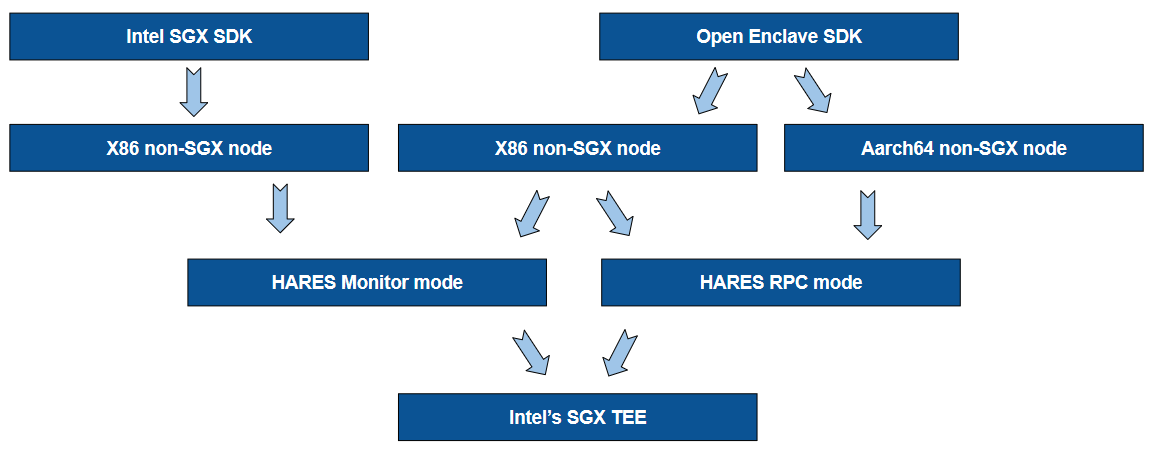
\includegraphics[scale=1.3]{figures/Arch_support_sgx2.png}
		\caption{Architecture supported by different modes of \monitor.} 
		\label{fig:arch_supported}
	\end{figure}

    As depicted in Figure \ref{fig:arch_supported}, the \textsc{Monitor} mode is applicable to the  x86 non-SGX nodes using the Open Enclave SDK and the Intel SGX SDK. On the other hand, the 'RPC' mode can be employed for both x86 and aarch64 based non-SGX nodes when using the Open Enclave SDK. 

    Before describing the design, We first explain the common terminologies used:

    \begin{enumerate}
        \item Client-node: This is a non-SGX node that requires SGX functionality. The SGX-based user application is initially launched on this node, and the execution context is migrated whenever an enclave function needs to be executed.
        \item Server-node: This is the SGX node responsible for facilitating SGX functionality. It remains in an idle state until a request comes from the client node.
        \item \monitor monitor: The monitor process is a Ptrace-based tool that suspends and resumes the user's SGX-based application while migrating between nodes. Additionally, it manages inter-node communication across nodes for enclave offloading. 
    \end{enumerate}
    
    We now discuss the two distinct modes of \monitor in the following sections. 

    \section{Monitor mode of \monitor for Homogeneous migrations} \label{ase: Monitor mode}
    As discussed in Section \ref{ase:Intel SGX SDK}, the Intel SGX SDK incorporates an Enclave Description Language (EDL) file to establish interfaces between the untrusted and trusted components of applications. This SDK offers support for both "Call by value" and "Call by reference" argument types for ecalls and ocalls functions. Within the SDK, the sgx\_edger8r tool plays a critical role by generating wrappers to facilitate interactions with the underlying SGX driver. However, a noteworthy point is that in these wrappers, the arguments provided by the user functions, whether passed by value or by reference, are directly forwarded to the underlying SGX interface. As a result, to ensure the smooth transition of application execution between nodes, the \monitor must maintain memory consistency across nodes. This becomes particularly critical when dealing with function calls that involve memory pointers. The preservation of memory coherence is essential to guarantee the correct and expected behavior of the application. This maintenance of memory consistency is a key aspect of the \monitor's \textsc{Monitor} mode.

    \subsection{High level design of Monitor mode} \label{ase: highlevel_design_monitor}
    The Figure \ref{fig:MonitorArch} shows the architecture of \monitor's \textsc{Monitor} mode. The mode operate as follows:

\afterpage{
    \begin{figure}[H]
    \centering
	\rotatebox{270}{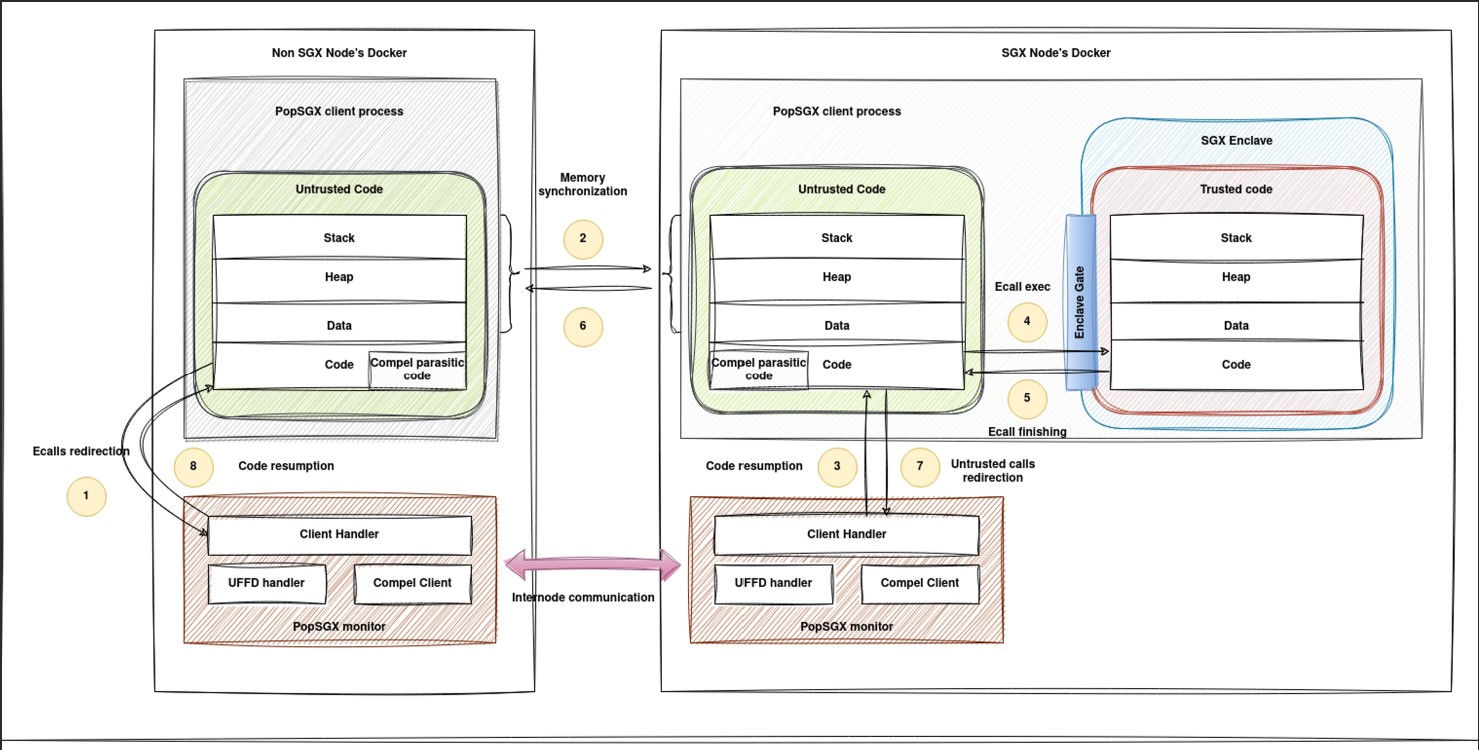
\includegraphics[scale=1.2, height=0.7\textwidth]{figures/monitor_arch_mini.jpg}}
	\caption{Architecture of \monitor's Monitor mode.} 
	\label{fig:MonitorArch}
	\end{figure}
}

    \begin{enumerate}
        \item As a starting point, the user must provide the enclave call instructions and their corresponding return instructions to the \monitor framework on both the server and the client nodes. 
        \item The client-side and server-side \monitor will have different behaviours. Initially, the client-side will set breakpoints for all the user-provided enclave instructions before launching the user's application. In contrast, the server-side will pause the application and await a request from the client side.
        \item The client \monitor upon capturing the execution of the enclave call triggered by the breakpoint, will then proceed to request the server \monitor to execute the enclave function.
        \item The server \monitor will initiate memory and register state synchronization before proceeding to execute the enclave call.
        \item Upon successful execution of the enclave call, the execution flow will return to the client-side \monitor. The client \monitor will then follow the same steps as the server \monitor, including memory and register state synchronization, and continue execution until the next breakpoint is encountered.
        \item Steps from (3) to (5) will be repeated whenever the client \monitor encounters an enclave call execution.
    \end{enumerate}

    \subsection{Memory Synchronization by \monitor}
    In order for the \monitor to offload the enclave functions, which may involve both call by value and call by reference arguments, it is essential to perform memory synchronization each time the execution transitions between different nodes, whether on the server or client side. 
    
    Memory synchronization is indeed a resource-intensive and time consuming process, demanding the maintenance of a consistent view of numerous pages across various Virtual Memory Area (VMA) regions, which can be quite extensive in size. In the Linux kernel, VMAs are used to track a process's memory mappings. Each process has separate VMA regions for different types of memory, including stack, heap, file-backed, and others. Each VMA is characterized by a starting address, size, permissions, and control flags. Some VMAs, like stack and heap, exhibit dynamic changes in size, expanding or shrinking, while other VMA types, such as file-backed, may be created or deleted during the course of a process's lifetime.

    \monitor must ensure that the most recent state of these VMAs remain consistent across the nodes, including both size and content. To extend the size of a specific region, the brk system call \cite{systemcall::brk} can be employed, and similarly, to create new regions, the mmap system call \cite{systemcall::mmap} is used. The contents can be updated with the help of calls such as process\_vm\_readv \cite{processVmReadv} and process\_vm\_writev \cite{processVmWritev}. Importantly, all of these calls must be executed within the context of the user application, and this is where the application of compel's \cite{COMPEL} parasitic injection is effective. 
    
    This is depicted in Figure \ref{fig:vmas_incremental}. Initially, there are five VMA regions. After the ecall execution on the remote, the extended heap (highlighted in green) is propagated to the Client node (marked in orange). Before offloading another ecall function, the client generates a new VMA region of the file-backed type, which is then sent to the remote node. This process continues until the application completes execution.

    \begin{figure}[htb]
	    \centering
		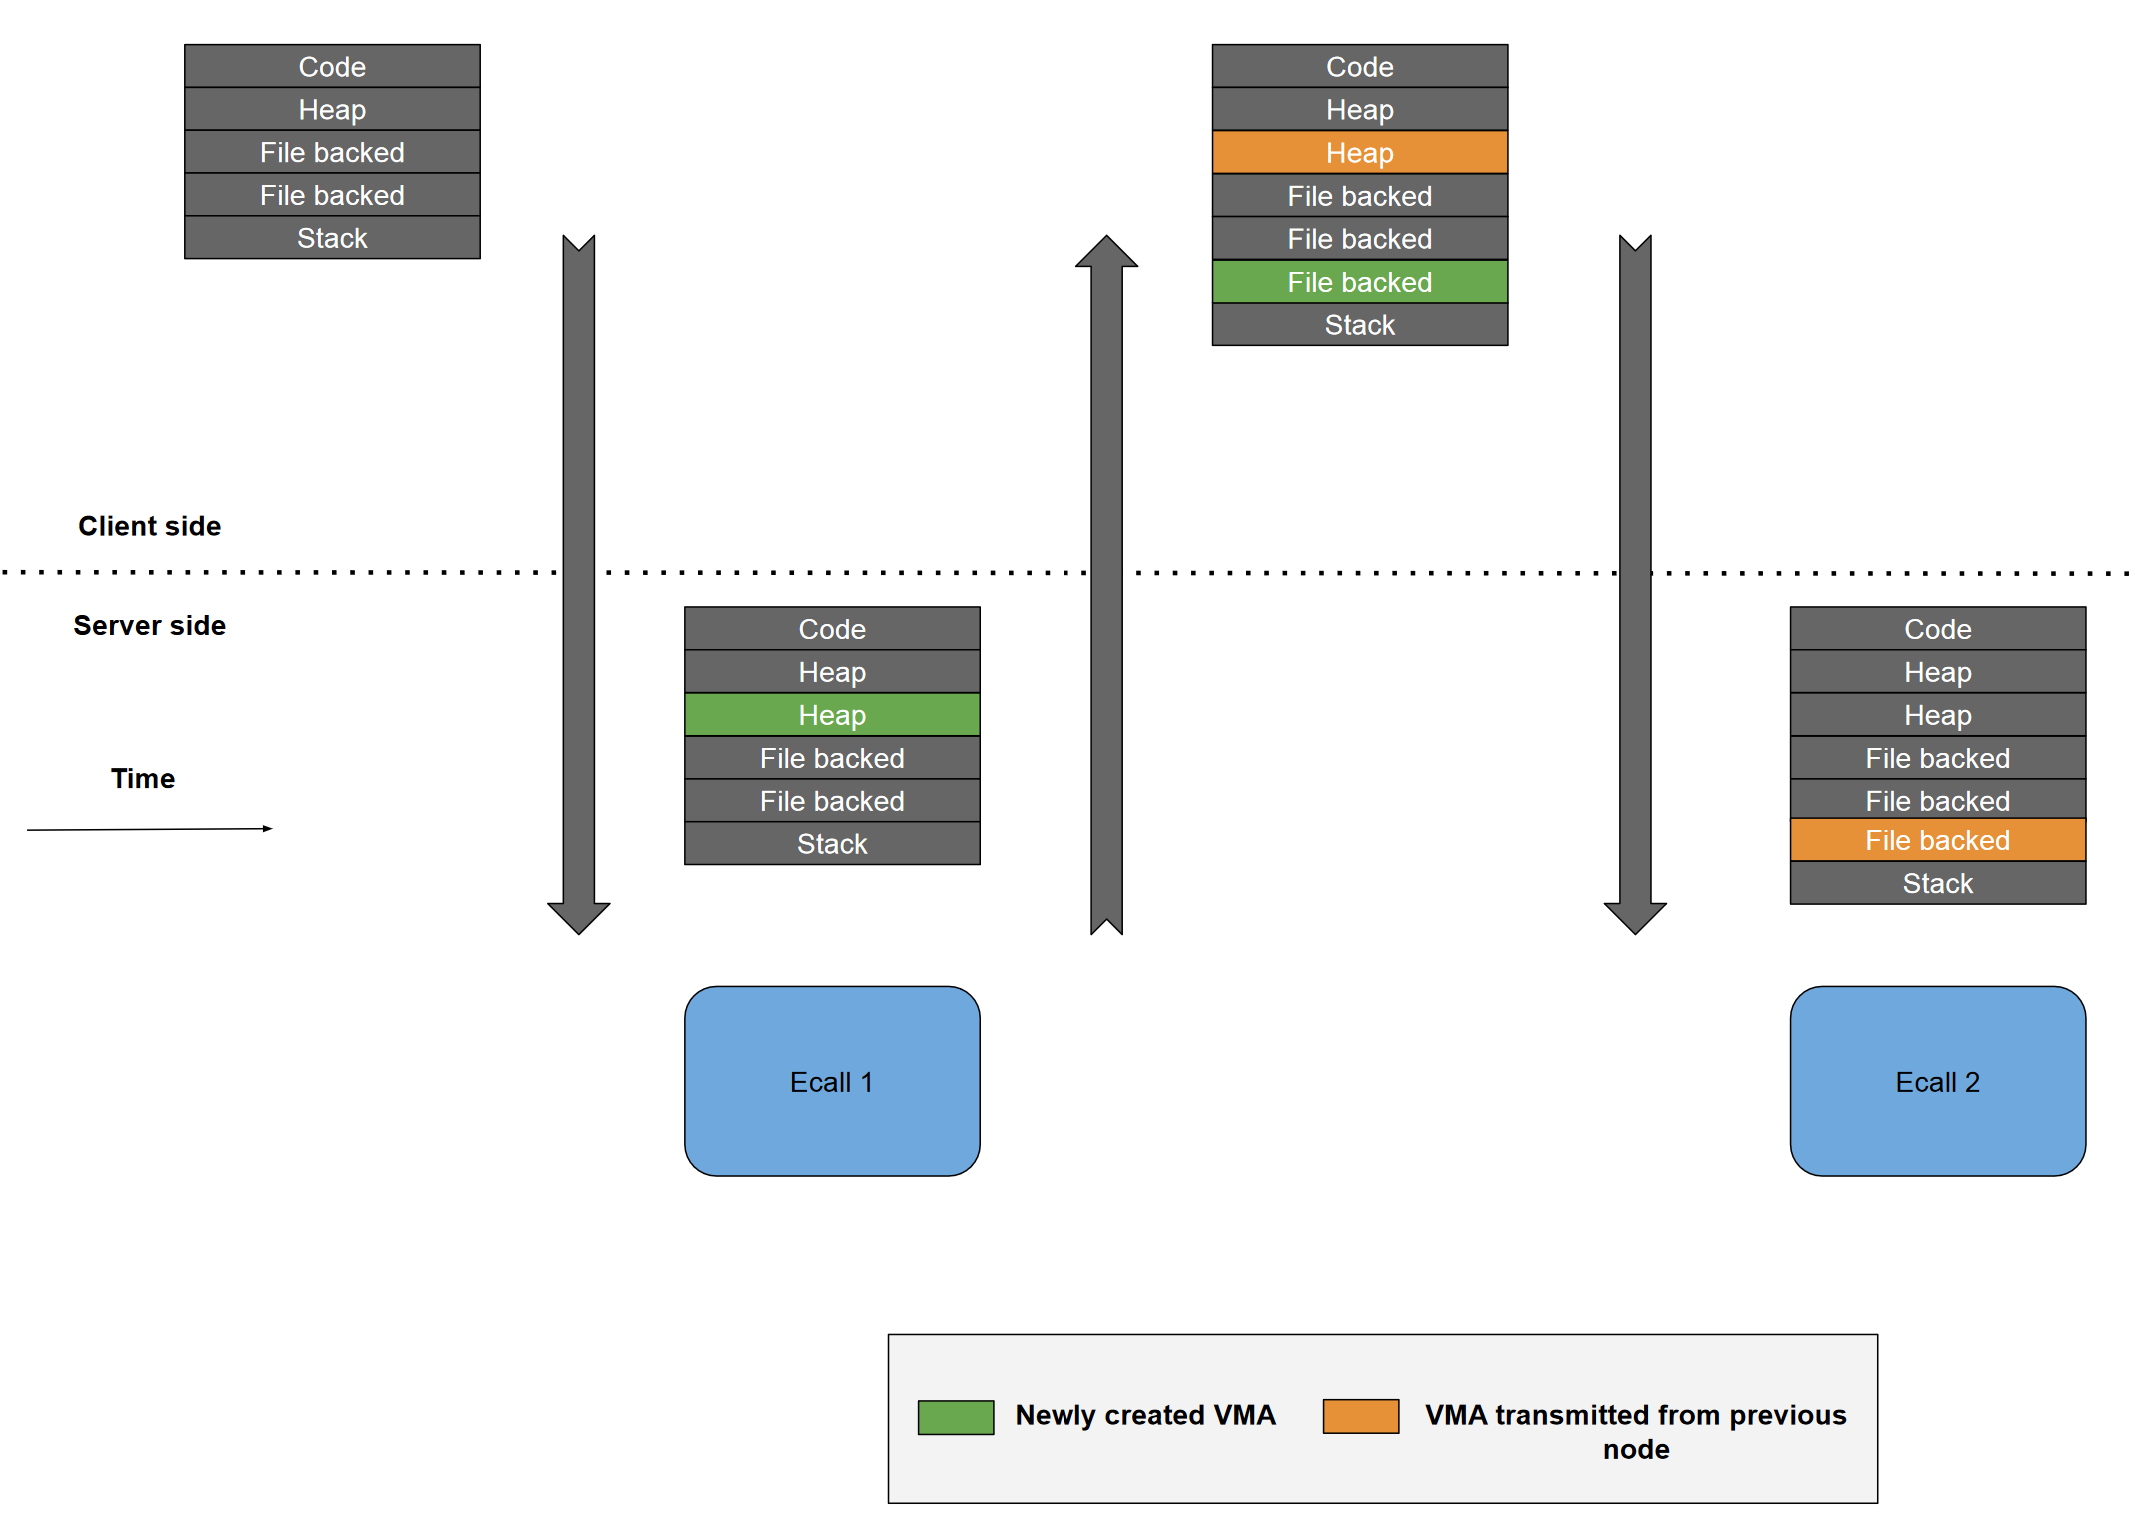
\includegraphics[scale=0.7]{figures/incremental_vmas.png}
		\caption{Incremental updates of VMA.} 
		\label{fig:vmas_incremental}
	\end{figure}

    \subsection{Faster memory synchronization}
    An application served by \monitor may involve numerous enclave function calls, necessitating frequent switches in execution context to a different node. During each of these execution context switches, transferring the entire process memory from one node to another is highly inefficient, and can result in significant latency. Therefore, the memory synchronization technique chosen by the \monitor framework should prioritize efficiency and speed. Minimizing performance degradation for users is essential, and a robust, optimized memory synchronization mechanism can significantly enhance the overall efficiency and responsiveness of the framework.

    One way to optimize memory synchronization is by transferring only the pages that have changed since the resumption of execution context on this node until the execution context switches to a different node. This ensures that the pages are synchronized across both the server and client sides. The Figure \ref{fig:pages_incremental} depicts the optimized memory synchronization. Initially, two new pages are created (highlighted in green) and sent to the server side (marked in yellow). Following this, an Ecall is executed, resulting in the generation of another page (depicted in green), and this process continues.

    \begin{figure}[htb]
	    \centering
		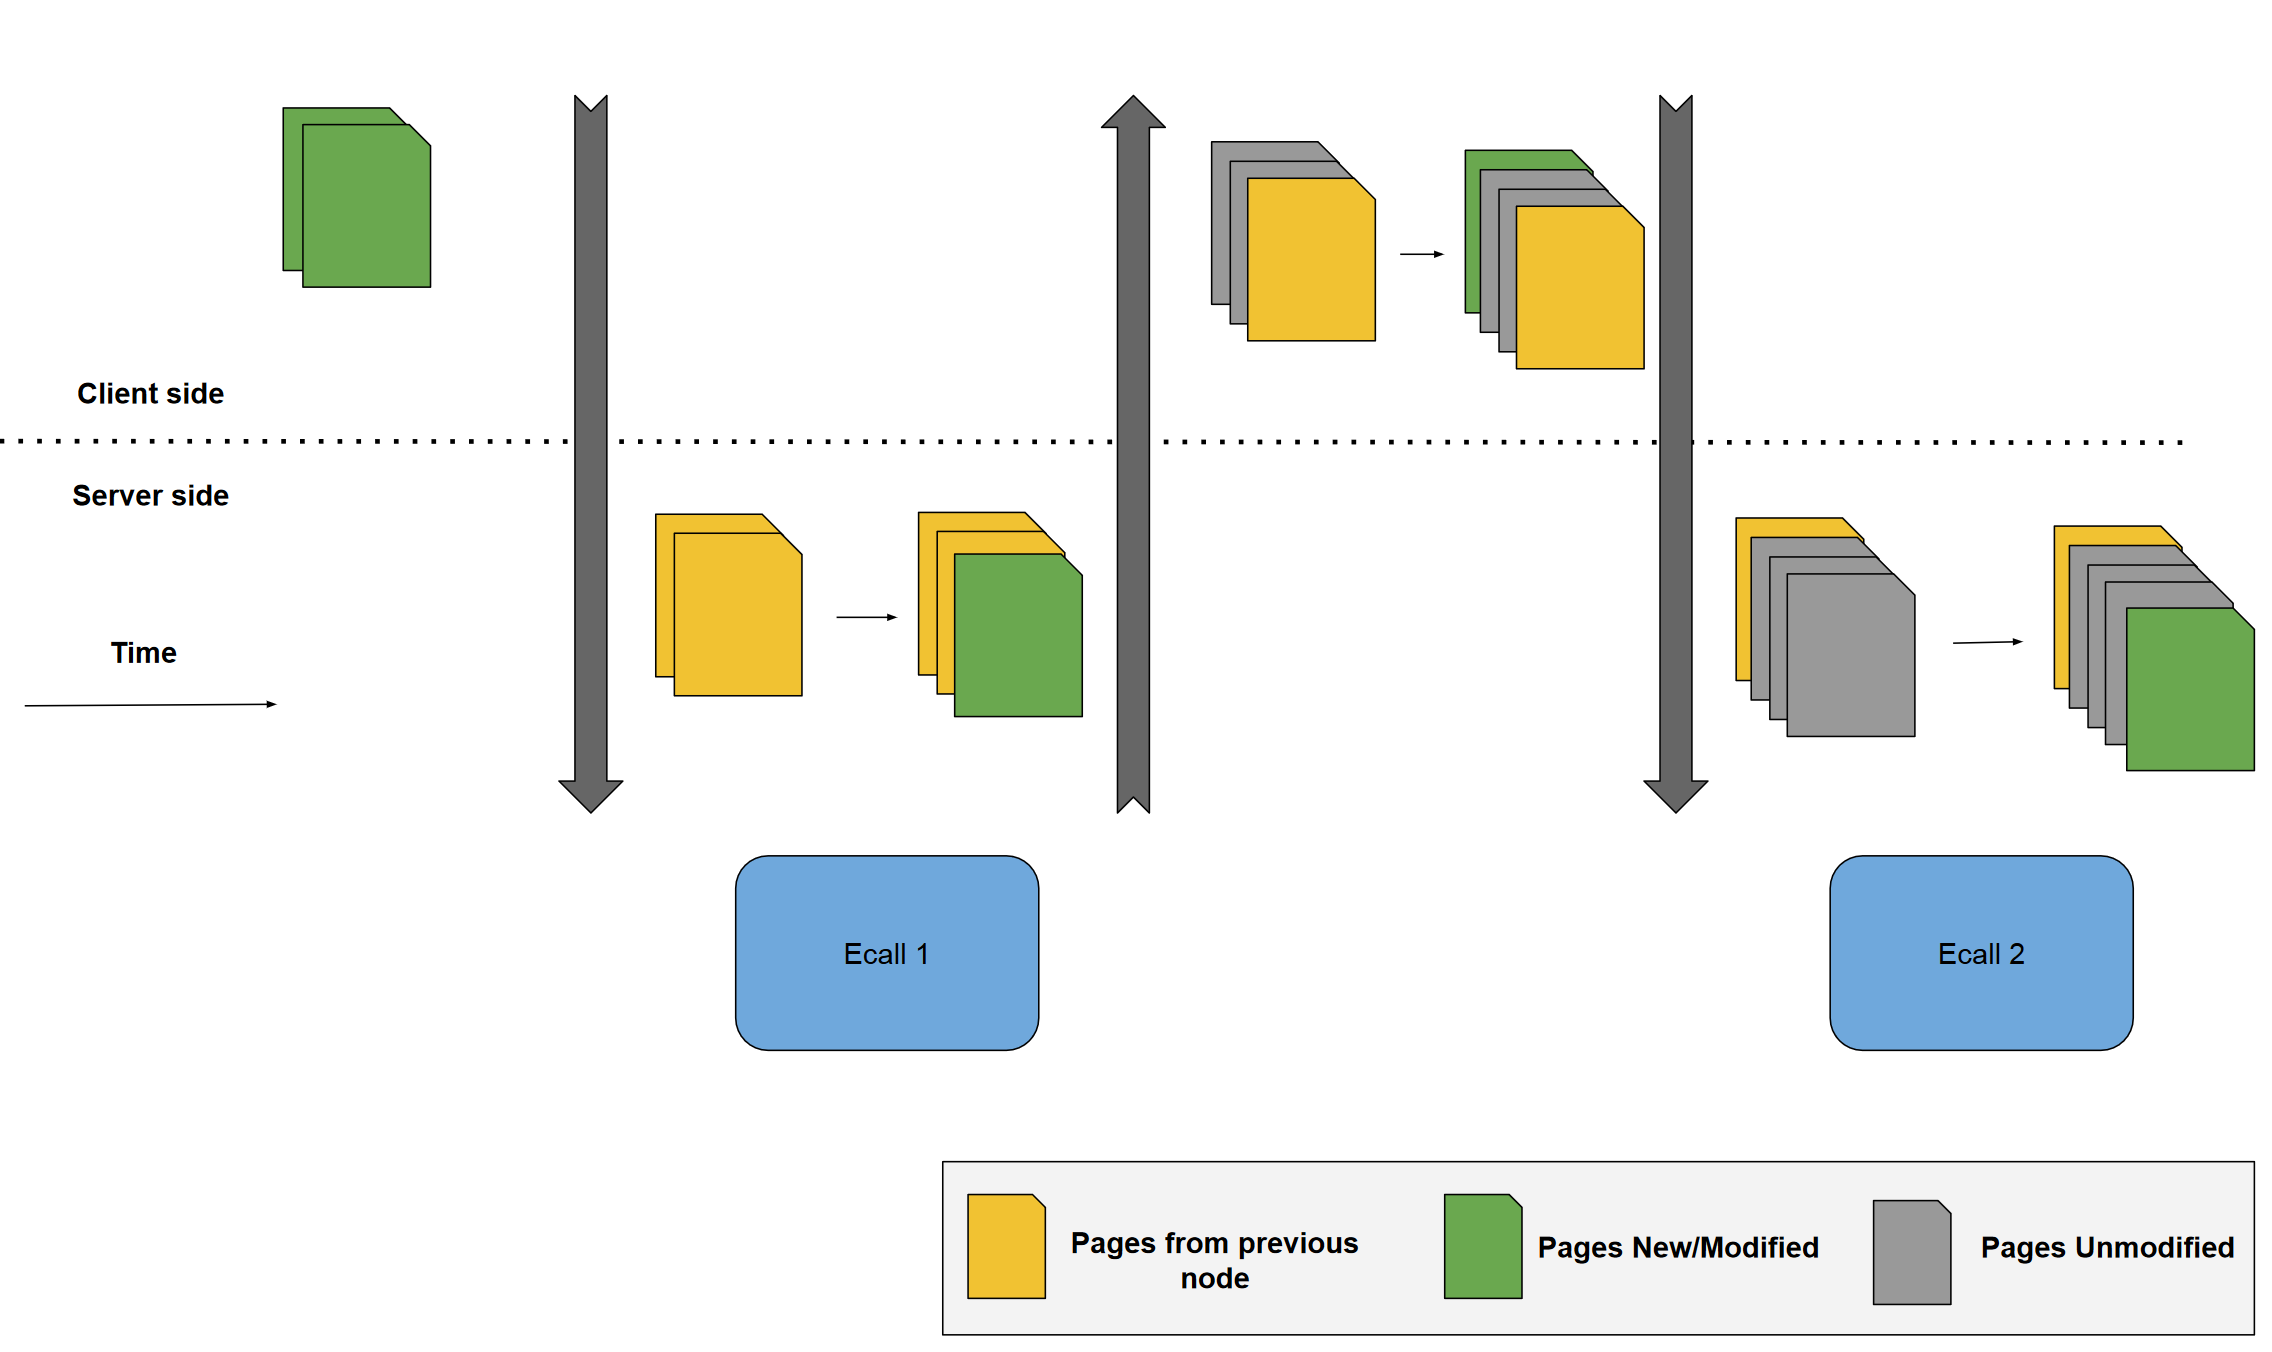
\includegraphics[scale=0.7]{figures/incremental_pages.png}
		\caption{Incremental update of pages.} 
		\label{fig:pages_incremental}
	\end{figure}


    In order to identify the pages that have been altered, \monitor employs a separate dedicated thread for handling page faults in the user space using userfaultfd, as mentioned in Section \ref{ss:Userfaultfd}. The \monitor will write-protect all pages every time code resumes on a particular node after migration. The pages that experience faults are identified as modified pages.

    \section{RPC mode for Heterogeneous migrations} \label{ase: RPC mode}
    The Open Enclave SDK supports Trusted Execution Environments (TEEs) for both x86 and aarch64 platforms. Aarch64 applications can leverage Arm's TrustZone technology, while x86 applications can utilize Intel's SGX (Software Guard Extensions). However, it's essential to note that applications compiled for one architecture (e.g., Aarch64) cannot use the TEE of another architecture (e.g., Intel's SGX), and vice versa. This is the precise challenge that \monitor aims to address. 

    \monitor tackles the challenge of executing enclave functions across different architectures (Aarch64 and x86) using the Remote Procedure Calls (RPCs) method \cite{Remote-procedure-call}. RPCs enables procedures to be executed in the address space of a remote process, as if they were executed in the local address space. This remote process can be situated either locally or remotely.

    By converting the enclave functions called from Aarch64 into RPCs, \monitor enables these enclave functions to be executed across platforms, allowing them to execute within Intel's SGX on the x86 platform. This approach helps bridge the architectural gap and facilitates the execution of enclave functions across ISA-different platforms. 

    \subsection{Serialization of Arguments for RPC by Open Enclave}
    To enable an enclave function to execute as an RPC function effectively, it is crucial that all arguments, whether passed by call by value or call by reference, undergo serialization before they are transmitted across different hardware.

    \begin{figure}
    \begin{tcolorbox}
    \begin{verbatim}
trusted {
    public int seal_data(int sealPolicy,
                [in, size = opt_msg_len] unsigned char* opt_mgs,
                size_t opt_msg_len,
                [in, size = data_size] unsigned char* data,
                size_t data_size,
                [out] data_t* sealed_data);

    public int unseal_data([in] const data_t* sealed_data,
                const int optional_msg_flag,
                [out] data_t* output_data);
};
    \end{verbatim}
    \end{tcolorbox}
    \caption{Open Enclave configuration file for Data Sealing application \cite{Data-Sealing}.}
    \label{fig:Data Sealing oe config}
    \end{figure}
    
    The auto-generated wrapper code provided by the Open Enclave SDK already performs
    some level of argument serialization before invoking the enclave function. Before we proceed further, let’s examine what this serialization process entails and how it contributes to the functioning of enclave functions in an RPC context.

     Figure \ref{fig:Data Sealing oe config}, shows the EDL (Enclave Description Language) configuration file for the Data Sealing application. Our focus will be on the seal\_data function. This function takes five arguments, of which the first four arguments are provided by the user, while the last argument sealed\_data is populated by the enclave function post execution. It is noteworthy that the arguments opt\_msg, data, and sealed\_data are passed by reference.

    \begin{figure}
    \begin{tcolorbox}
    \begin{verbatim}
    /**** ECALL marshalling structs. ****/
    typedef struct _seal_data_args_t
    {
        oe_result_t oe_result;
        uint8_t* deepcopy_out_buffer;
        size_t deepcopy_out_buffer_size;
        int oe_retval;
        int sealPolicy;
        unsigned char* opt_mgs;
        size_t opt_msg_len;
        unsigned char* data;
        size_t data_size;
        data_t* sealed_data;
    } seal_data_args_t;
    \end{verbatim}
    \end{tcolorbox}
    \caption{Marshalling struct auto-generated by Open Enclave}
    \label{fig:Marshalling struct}
    \end{figure}


    The ECALL marshalling structure, depicted in Figure \ref{fig:Marshalling struct}, is an auto-generated structure created by Open Enclave for passing arguments into enclave calls. Before passing this structure to the ECALLs, its content needs to be marshaled and serialized. The method employed by Open Enclave for this purpose is illustrated in Figure \ref{fig:OE-Serialization}.

\afterpage{
    \begin{figure}[H]
    \centering
    \begin{subfigure}{\textwidth}
        \centering
        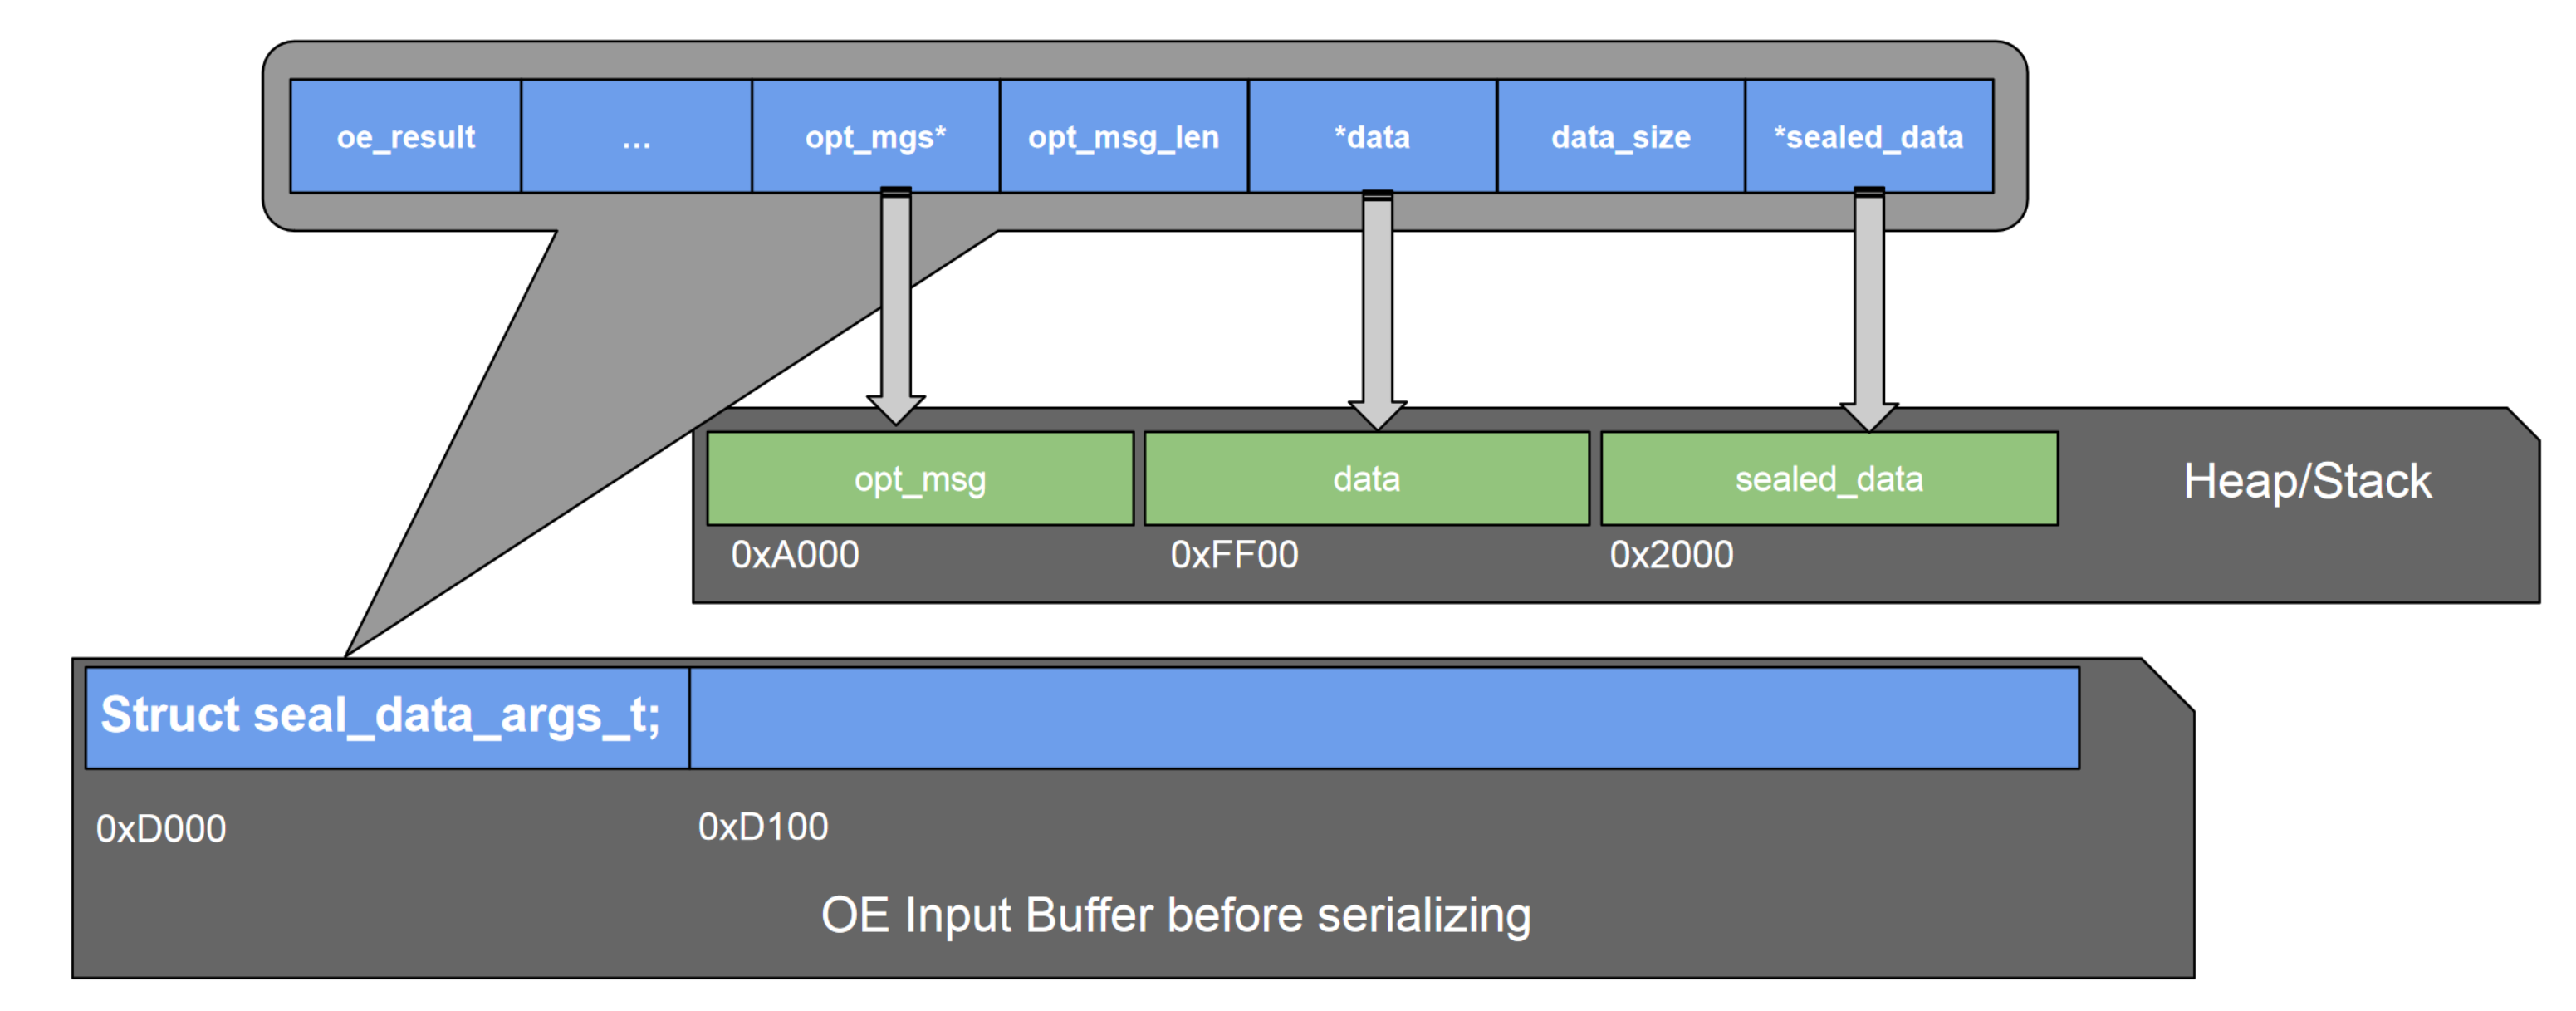
\includegraphics[scale=0.4]{figures/rpc_buffer_before_serialization.png}
        \caption{Open Enclave's buffer before serialization}
        \label{sfig:rpc_buffer_before_serialization}
    \end{subfigure}
    \\[30pt]
    \begin{subfigure}{\textwidth}
        \centering
        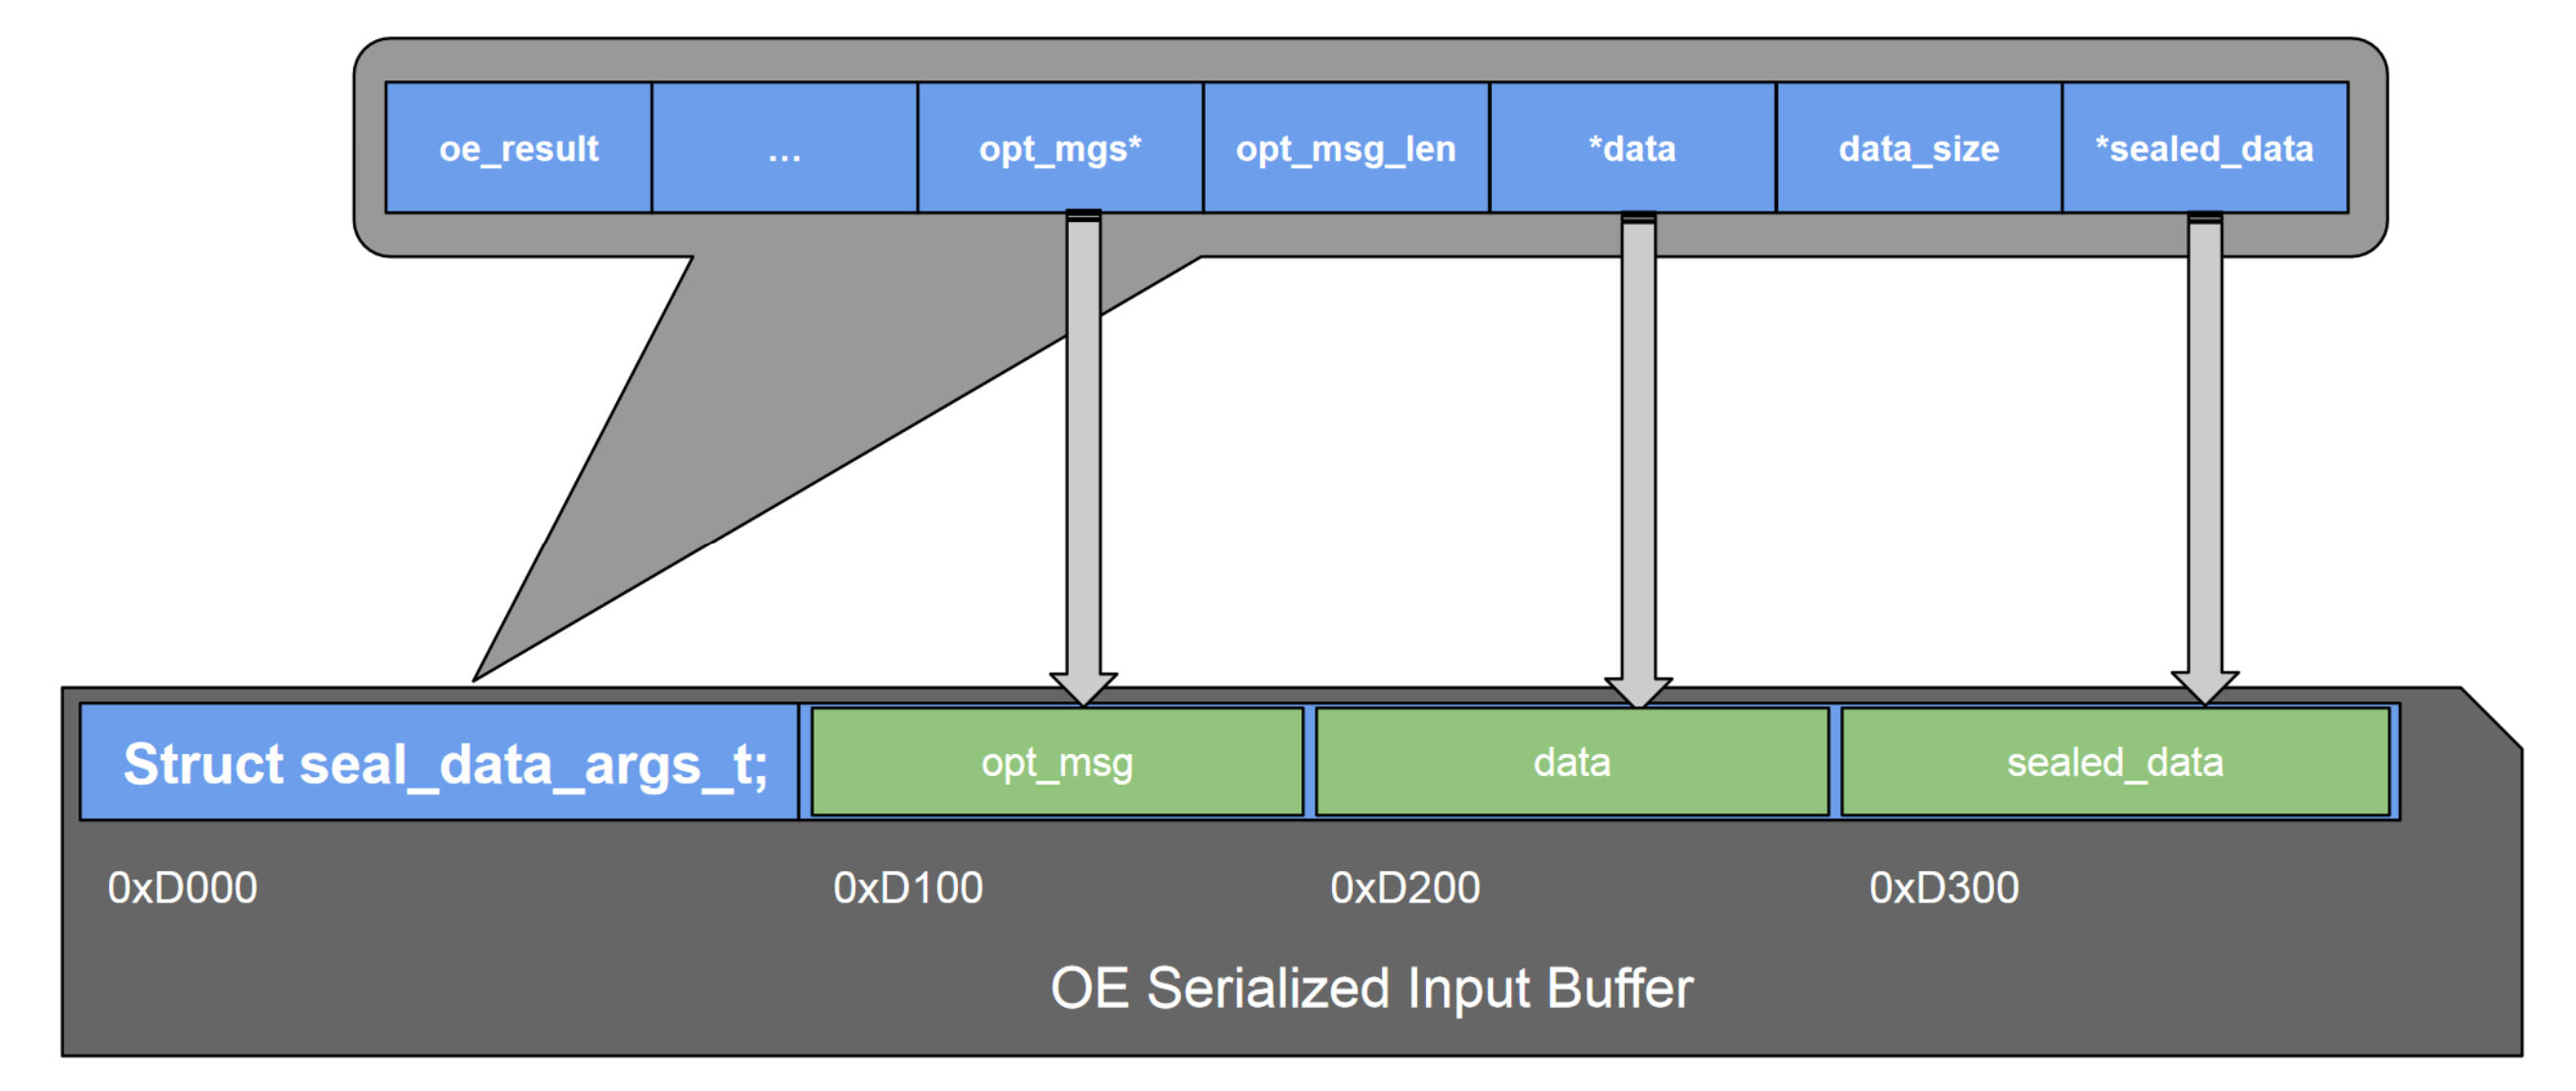
\includegraphics[scale=0.4]{figures/rpc_buffer_after_serialization_oe.png}
        \caption{Open Enclave's buffer after serialization}
        \label{sfig:rpc_buffer_after_serialization_oe}
    \end{subfigure}

    \caption{Serialization by Open Enclave}
    \label{fig:OE-Serialization}
    \end{figure}
}

    At first, Open Enclave allocates a buffer in the heap with sufficient size to accommodate not only the marshalling structure holding the function's arguments, but also the size of contents that could be dereferenced by the pointers in the arguments. As seen in Figure \ref{sfig:rpc_buffer_before_serialization}, the OE Input Buffer before serializing holds the marshalling structure at address 0xD000 and the content to be dereferenced at 0xD100. At this point, the pointers within the marshalling structure still reference the memory addresses initially created by the user. For instance, opt\_msg is at 0xA000, while data is at 0xFF00. As part of serialization, all contents pointed to by the user-given arguments will be placed within the Open Enclave-generated intermediary buffer, and the references within the marshalling structure will be changed to the contents copied within this intermediary buffer. 
    
    For example in Figure \ref{sfig:rpc_buffer_after_serialization_oe}, the 'opt\_msg' pointer now points to 0xD100, the 'data' pointer points to 0xD200, and so on. If there are any nested pointers, their contents will also be copied, and their references will be adjusted accordingly

    \subsection{Pointer adjustment and readjustment by \monitor} \label{adj_and_readj_of_monitor}
    \afterpage{
    \begin{figure}[H]
        \centering
        \begin{subfigure}{\textwidth}
            \centering
            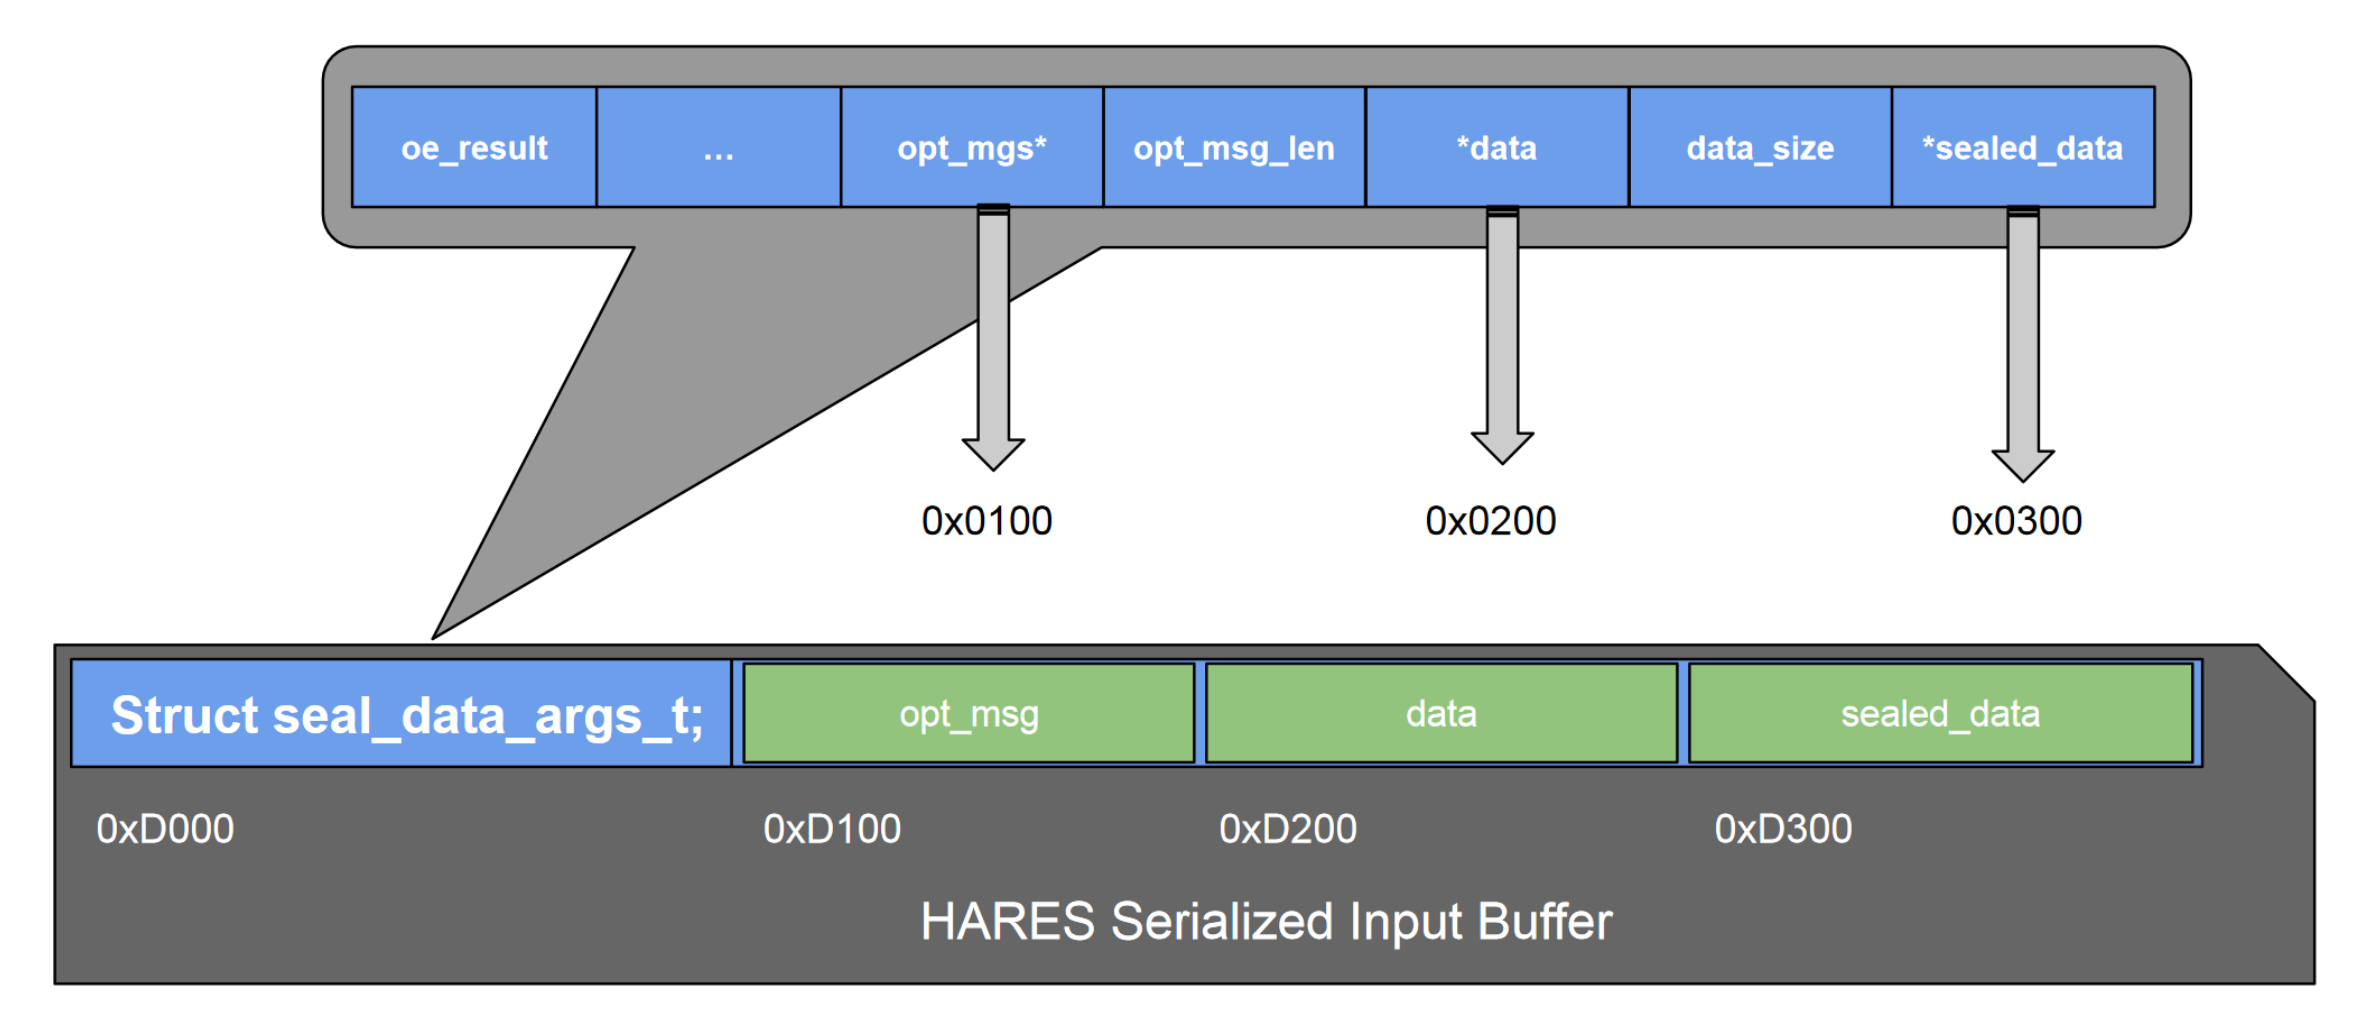
\includegraphics[scale=0.4]{figures/rpc_buffer_hares_serialization.png}
            \caption{Open Enclave's buffer after \monitor adjustment in client}
            \label{sfig:rpc_buffer_hares_serialization}
        \end{subfigure}
        \\[30pt]
        \begin{subfigure}{\textwidth}
            \centering
            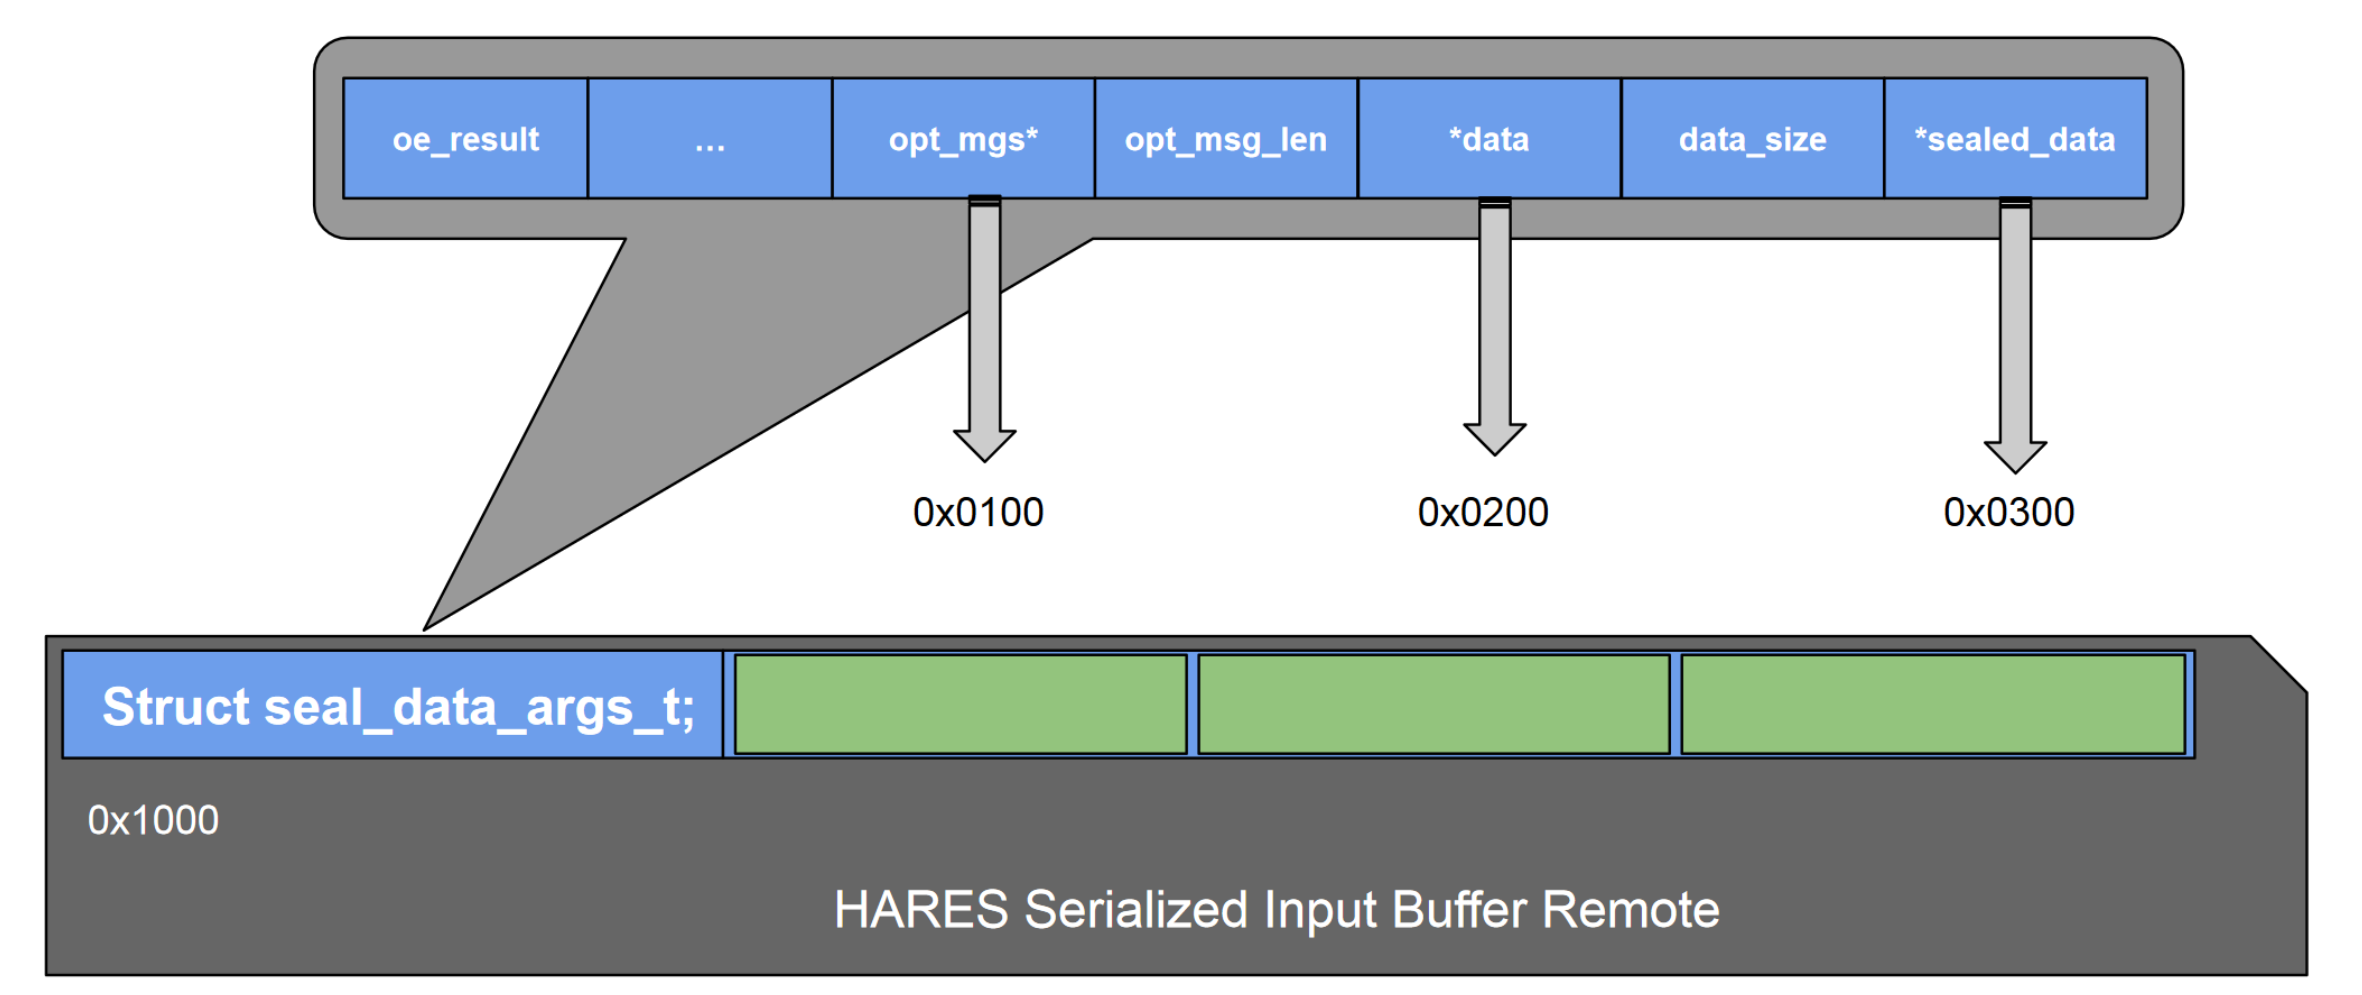
\includegraphics[scale=0.4]{figures/rpc_buffer_hares_before_readjustment.png}
            \caption{Open Enclave's buffer with \monitor before readjustment in server}
            \label{sfig:rpc_buffer_hares_before_readjustment}
        \end{subfigure}
        \\[30pt]
        \begin{subfigure}{\textwidth}
            \centering
            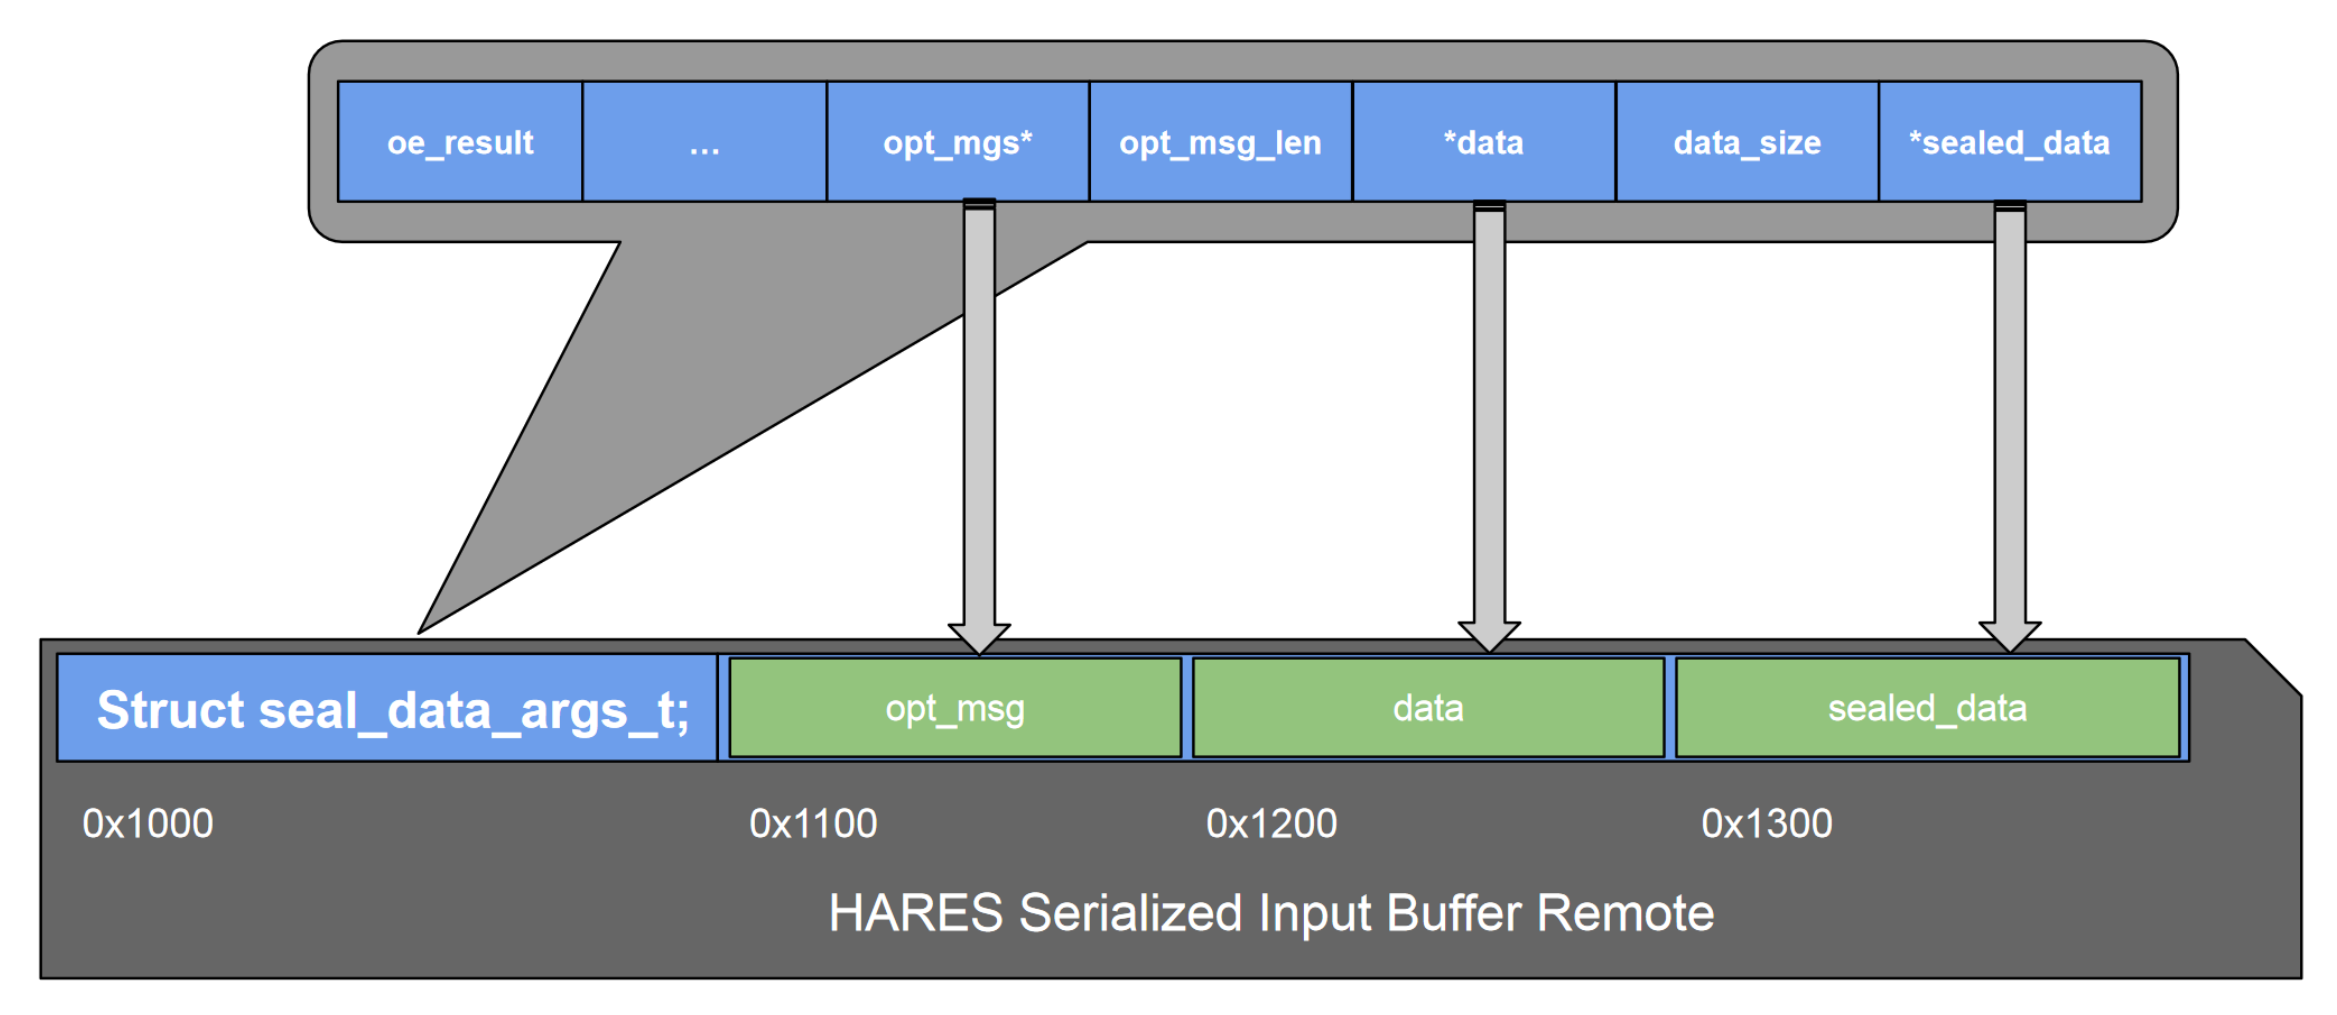
\includegraphics[scale=0.4]{figures/rpc_buffer_hares_after_readjustment.png}
            \caption{Open Enclave's buffer \monitor readjustment in server}
            \label{sfig:rpc_buffer_hares_after_readjustment}
        \end{subfigure}
        \\[20pt]
        \caption{Open Enclave's buffer manipulation.}
        \label{fig:HARES-Serialization}
    \end{figure}
}

    The references made by the pointers within the marshalling structure, however, lose their meaning when passed to the remote node. Hence, an adjustment of pointers needs to be made by the \monitor before transferring. 
    
    Figure \ref{fig:HARES-Serialization} illustrates this process. Pointers within the marshalling structure are assigned addresses relative to the buffer's starting address (0xD000 in this case). After \monitor's adjustment from Figure \ref{sfig:rpc_buffer_hares_serialization}, we observe that pointers such as 'opt\_msg' have a value of 0x0100, 'data' has 0x0200, and so on.
    
    This serialized and adjusted buffer is then passed from the client node to the server node, where a readjustment takes place. A new temporary buffer of the exact size is created, holding the data passed from the client node to the server side. In Figure \ref{sfig:rpc_buffer_hares_before_readjustment}, the newly created buffer is at the address 0x1000, with the pointers still holding the adjusted relative address values such as 0x0100, 0x0200, and so on. These adjusted values are then further readjusted to point within this temporary buffer, ensuring that subsequent dereferences pose no issues and remain consistent with memory accesses. The pointers, after readjustment, will have values such as 0x1100, 0x1200, and so on. For nested pointers, the adjustment and re-adjustment have to be made in a similar fashion. The same could be employed for ouptut arguments such as the argument pointer sealed\_data of the seal\_data function in the Figure \ref{fig:Data Sealing oe config}.

    \chapter{Implementation} \label{ch:implementation}
    \monitor was developed to extend SGX capabilities to devices that lack native SGX support, effectively enabling SGX offloading from non-SGX x86 or aarch64 devices. It provides two distinct modes: \textit{Monitor} and \textit{RPC}.

    This chapter delves into the intricacies of the \monitor's design, exploring both of its operational modes. Section \ref{ase:implementation of monitor mode} and its corresponding subsections delve into the implementation details of the monitor mode, while Section \ref{ase:implementation of rpc mode} elaborates on the intricacies of the RPC mode's implementation. 
    
    \section{Implementation of Monitor mode} \label{ase:implementation of monitor mode}
    The monitor mode provides a design that is internally framework-agnostic. It is accompanied by a "monitor" process that manages the execution migration  from one node to another while simultaneously ensuring memory synchronization. The modules used in the \textit{Monitor} mode are discussed in the following subsections.
    
    \subsection{Monitor's Configuration} \label{ase: Json Parser}
    
    \begin{figure}[htb]
        \centering
        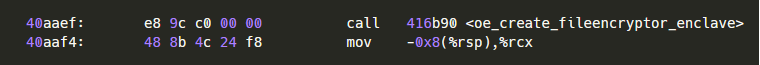
\includegraphics[scale=2.0]{figures/transisitonal_assembly_inst.png}
        \caption{Assembly instructions calling and returning from Enclave functions.} 
        \label{fig:transition_assembly}
    \end{figure}
 
    The \textit{Monitor} mode enables the transition of the execution context to a different node at a specific instruction. This instruction may involve calling an Enclave function, such as 0x40aaef in Figure \ref{fig:transition_assembly} (transition from client to server), or returning from the Enclave function, like 0x40aaf4 in Figure \ref{fig:transition_assembly} (Transition from server to client). To facilitate this transition, users of the \monitor need to make it aware of these transitional instructions. This is accomplished using a configuration file. The configuration file is in JSON format. An example configuration file used for a HelloWorld application is illustrated in Figure \ref{fig:config_monitor}, with the fields listed as follows:
    
    \begin{itemize}
        \item \texttt{main\_address}: Gives the address of the main function.
        \item \texttt{user\_args}: Provides the user arguments for starting \monitor's client application, which is the user application.
        \item \texttt{breakpoints}: Specifies the transitional instruction addresses. Odd instructions are considered as calls to Enclave Functions, and even instructions are considered as returns from Enclave functions.
    \end{itemize}
    
    \begin{figure}[htb]
        \centering
        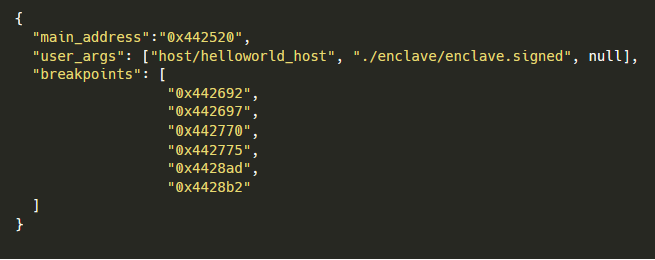
\includegraphics[scale=2.0]{figures/configuration_json.png}
        \caption{JSON-based configuration file of \monitor \textit{Monitor} mode.} 
        \label{fig:config_monitor}
    \end{figure}
    
    Configurations, such as the one in Figure \ref{fig:config_monitor}, will be parsed by the monitor process to set breakpoints and transition the execution context.

    \subsection{The Compel Handler of \monitor} \label{ase:compel handler}
    As described in Section \ref{ase:compel handler}, \monitor uses compel's parasitic injection mechanism to steal the userfault-fds and handle the extensions of the VMAs. Whenever the \monitor intends to execute a specific command through the parasitic code, it has to send the command along with the appropriate arguments. The commands used by \monitor are listed in Figure \ref{fig:comple_interface}. The purpose of individual commands is listed below:

    \begin{itemize}
        \item \texttt{PARASITE\_CMD\_GET\_STDUFLT\_FD} is a command used for the registration of the userfault-fd (uffd). The arguments used include the pointer where \textsc{fd} is to be filled, the starting address, and the number of pages for \textsc{uffd} registration.
        \item \texttt{PARASITE\_CORRECT\_HEAP\_OFFSET} is a command used to extend the size of the heap. The argument is the number of pages to extend.
        \item \texttt{PARASITE\_CMD\_REM\_STDUFLT\_FD} is a command used to remove the userfault-fd registration. The arguments are the file descriptor, the starting address, and the number of pages for the de-registration of \textsc{uffd}.
        \item \texttt{PARASITE\_CMD\_CREATE\_MMAP} is a command used to create a new MMAP-ed region. The arguments include the desired address and the number of pages to be allocated for this memory region.
    \end{itemize}


    \begin{figure}[htb]
        \centering
        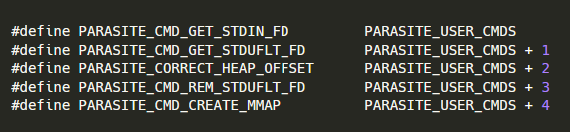
\includegraphics[scale=2.0]{figures/compel-macros.png}
        \caption{Compel's interface commands by \monitor.} 
        \label{fig:comple_interface}
    \end{figure}

    Another crucial consideration is that during the registration of userfaultfd for all the write-permitted regions, we must ensure that we ignore the VMA of the user application that belongs to the parasitic code. Otherwise, the parasitic code would encounter a write fault and wait for \monitor to handle it through userfaultfd. However, by then \monitor would still be registering \textsc{uffd} for other regions of the user application, thus leading  to a deadlock.

    \subsection{Userfault handler thread of \monitor} \label{ase:userfaultfd handler}
    The userfault handler thread is responsible for handling all page faults of the application in the user space. All uffds maintained by the thread will be destroyed and re-registered whenever a new VMA has been destroyed or created respectively, facilitating easy maintenance of uffds. During a transition from a remote node to the node, all the pages within all VMA regions will be write-protected to identify the pages that will be modified. Figure \ref{fig:uffd_handler} illustrates that any writes further down the line until a transition to a remote node will trigger a page fault, and the pages will then be marked as modified, accompanied by write unprotection. Figure. \ref{fig:uffd_handler} illustrates this with green boxes.

    \begin{figure}[htb]
        \centering
        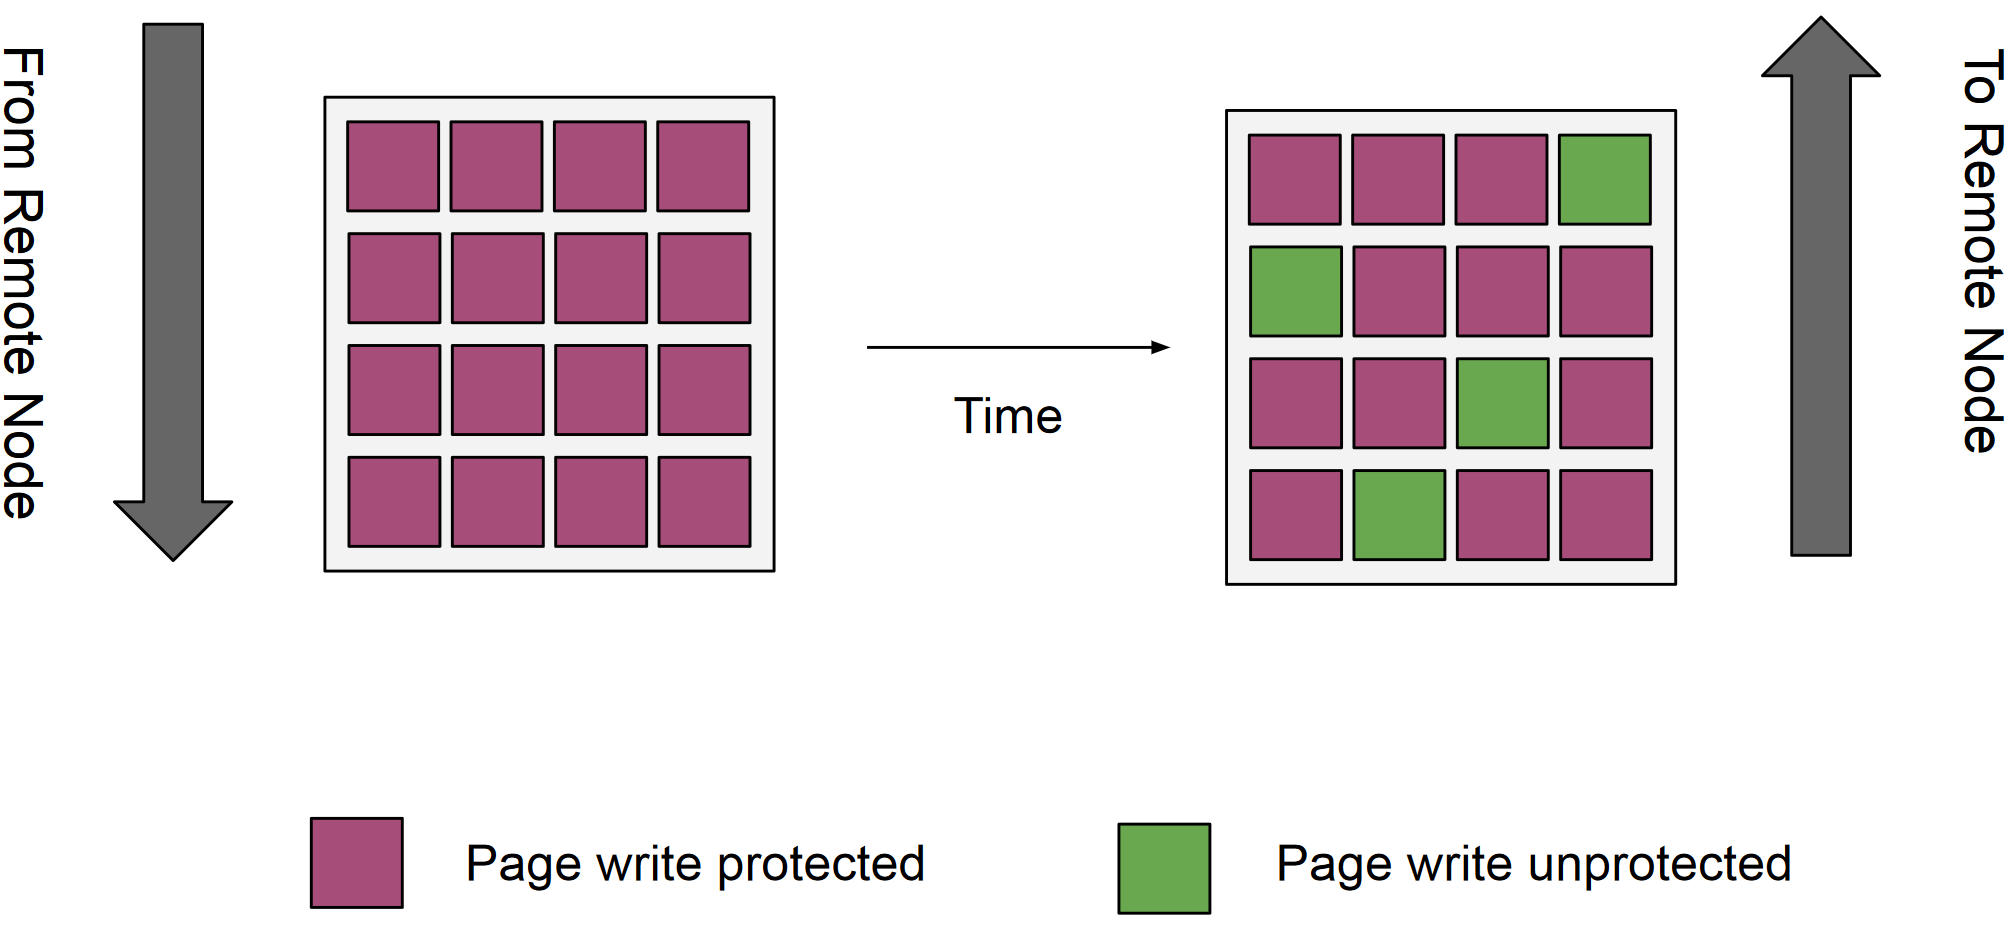
\includegraphics[scale=0.7]{figures/uffd_handler.png}
        \caption{UFFD handler handling pages.} 
        \label{fig:uffd_handler}
    \end{figure}

    Furthermore, the userfaultfd mechanism does not allow one to register for file-backed pages, and hence, all the pages within the VMA regions belonging to file-backed pages have to be sent every time during the transition. 
    
    \subsection{Memory synchronization APIs used} \label{ase:memsync_api}
    The \monitor framework utilizes inter-node TCP/IP APIs to transfer the necessary information for remote execution of the application, such as memory and register state, and to exchange synchronization messages. Optionally, \monitor allows establishing an SSL/TLS communication channel to secure the messages. 

    Table \ref{t:TPayload} lists the synchronization APIs used and their corresponding payload sizes. For convineince in presentation, The \monitor in the server will be referred to as \monitor-s, and similarly, the \monitor in the client will be called \monitor-c. Transitions can occur in both directions, with the REMOTE\_EXECUTE header being the first.  When transitioning from \monitor-c to \monitor-s, the instruction until which execution has to happen is sent as the payload. \monitor-s reads this payload to set a breakpoint in the application and facilitate the transition back to \monitor-c. Also, it’s worth noting that when transitioning from \monitor-s to \monitor-c, the payload could be empty because the application in the client will execute as long as it hits the breakpoint set by \monitor-c. 
    
    The second message header would be REMOTE\_REGS, with the payload consisting of the register states themselves. This information is needed to set the register sets of the application properly and execute the required portion of the code.
    
    \begin{table}[h]
	\centering
	\footnotesize
	\caption{Inter-node TCP/IP messages with its payload size.}
	\begin{tabular}{| c | c |} \hline
		  Messages & Bytes transferred\\ \hline \hline
        REMOTE\_EXECUTE  &  16 \\ \hline
        REMOTE\_EXECUTE\_REPLY  &  8 \\  \hline
        REMOTE\_REGS &  220 \\  \hline
        REMOTE\_REGS\_REPLY & 8 \\ \hline
        VMA\_FROM\_REMOTE &  16 \\ \hline
        VMA\_FROM\_REMOTE\_REPLY &  8\\ \hline
        VMA\_BUFFER\_HEADER & 28 \\ \hline
        VMA\_BUFFER\_HEADER\_ACK & 8 \\ \hline
        VMA\_BUFFER (Per page) & 5004\\ \hline
        VMA\_BUFFER\_ACK (Per Page) & 8 \\ \hline
        VMA\_TRANS\_ACK & 8\\ \hline
	\end{tabular}
	\label{t:TPayload}
    \end{table}
    
    The next message header is VMA\_FROM\_REMOTE, which indicates the number of VMA regions or pages that will follow in subsequent messages. The message header VMA\_BUFFER \_HEADER then provides additional information, such as the number of pages and the starting address of the application’s memory to follow in the subsequent message. The following message, VMA\_BUFFER, contains the payload of the page itself. Finally, the communication ends with the receiver side sending VMA\_TRANS\_ACK along with acknowledgment for each of the afore-mentioned message headers. 
    
    In Table \ref{t:TPayload}, the largest message is the VMA\_BUFFER message, which is 5004 bytes in size
    because it contains the page itself, which is typically 4096 bytes in size, along with additional information such as the page address.


    \subsection{Instruction Cleaner} \label{ase:inst_cleaner}
    \begin{figure}[htb]
        \centering
        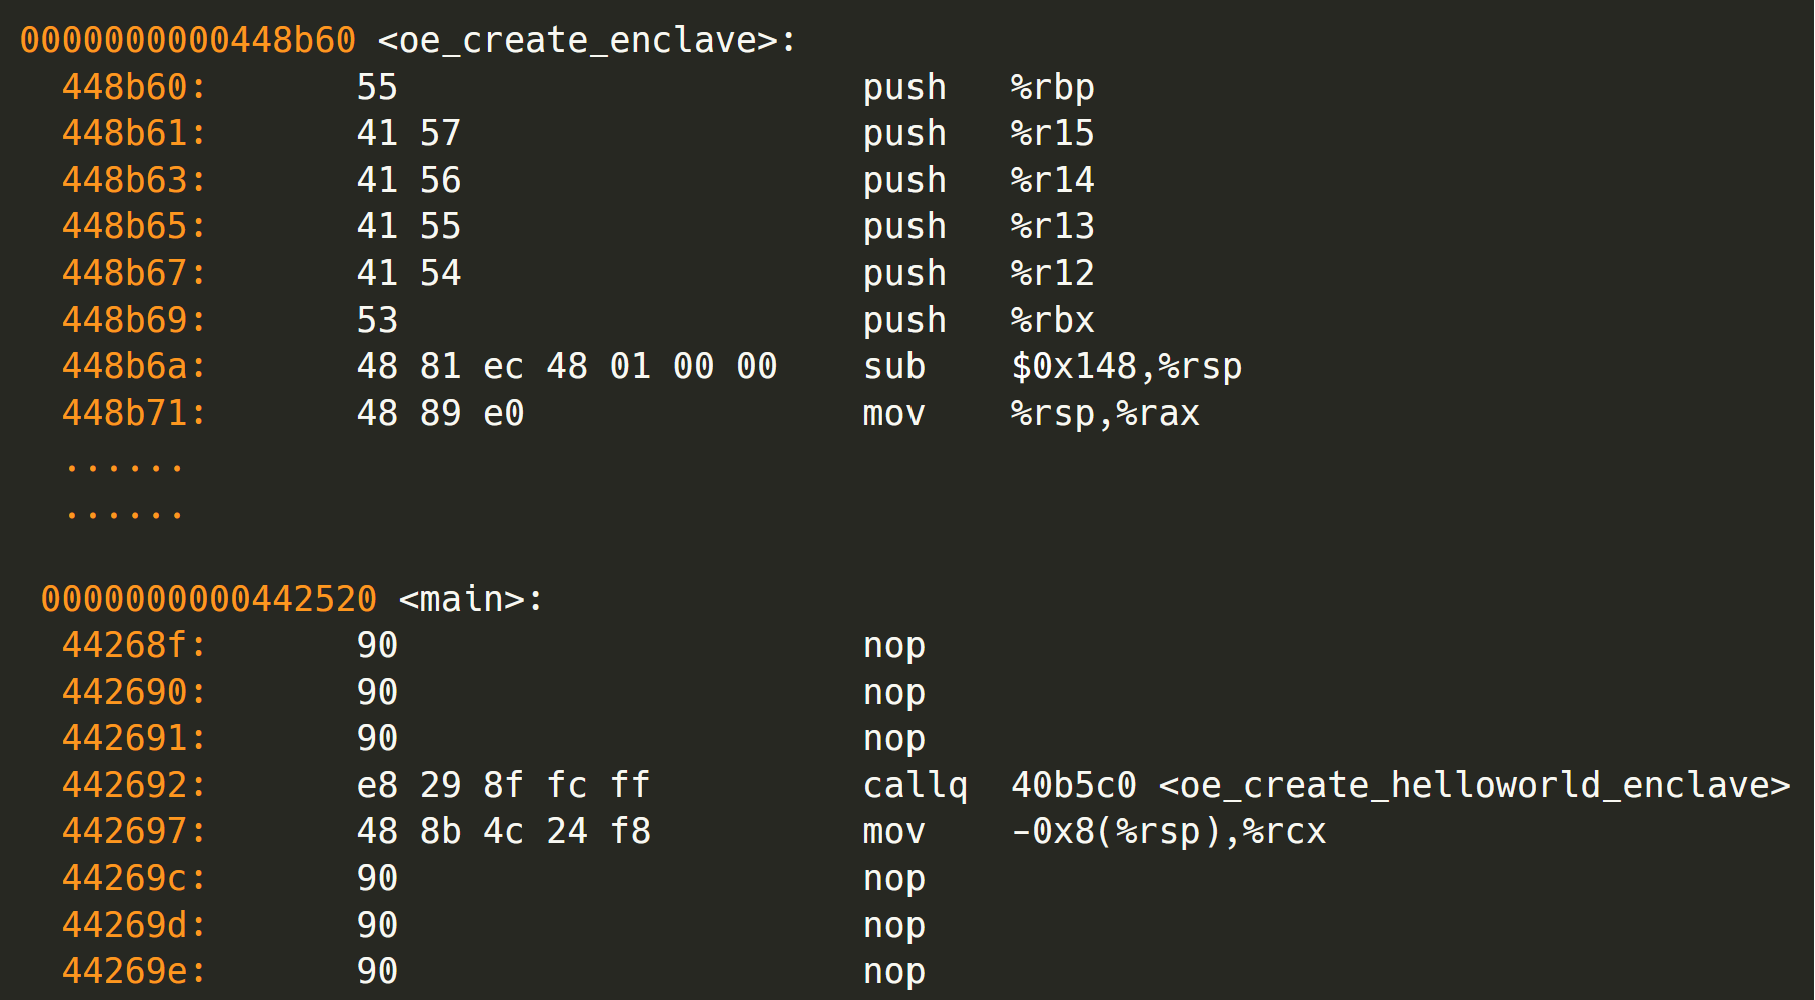
\includegraphics[scale=0.7]{figures/server_instruction_cleaned.png}
        \caption{Instructions cleaned in the server side.} 
        \label{fig:server_instructions}
    \end{figure}
    
    If we take a look at Figure \ref{fig:MonitorArch}, the server and the client side are bloated with instructions that aren't supposed to be executed on their respective ends. For instance, instructions belonging to the enclave wrapper code are not executed on the client side, and similarly, all instructions belonging to codes other than the enclave wrapper are not executed on the server side. Hence, these non-executed instructions are replaced with x86's NOP instruction using a cleaner script before deploying with the \monitor mode. Figure \ref{fig:server_instructions} and \ref{fig:client_instructions} show the cleaned assembly instructions where \textit{oe\_create\_enclave} is the wrapper for the enclave function, and main is the non-wrapper function displayed.

    \begin{figure}[htb]
        \centering
        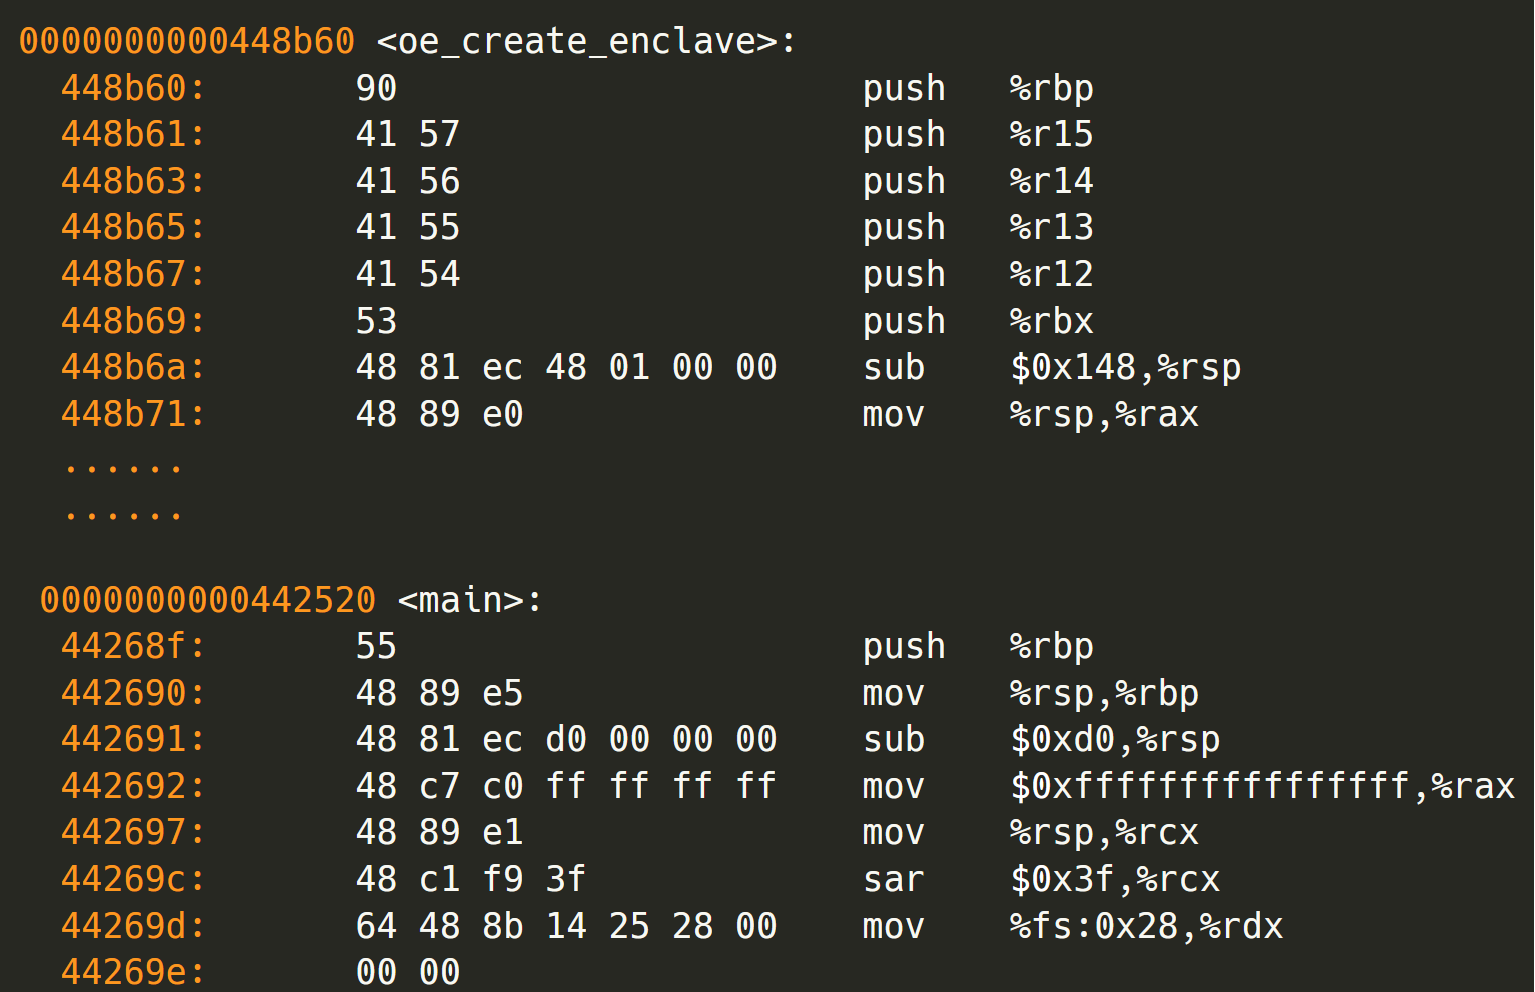
\includegraphics[scale=0.8]{figures/client_instruction_cleaned.png}
        \caption{Instructions cleaned in the client side.} 
        \label{fig:client_instructions}
    \end{figure}

    \section{Implementation of RPC mode} \label{ase:implementation of rpc mode} 
    Unlike the \textsc{Monitor} mode of the \monitor, where \monitor-c and \monitor-s monitor processes were required on both sides, the RPC mode modifies the wrapper code of the user applications. In this mode, the \monitor modified wrapper code residing on both sides handles all enclave offloading. To modify the wrapper code of the user application, the \monitor leverages and modifies the \textsc{oeedger8r} tool. \textsc{oeedger8r} is an auto code generator used by Open Enclave to generate the wrapper code that sets up a trampoline between the trusted and untrusted worlds. 

    \afterpage{
        \begin{figure}[htb]
            \centering
            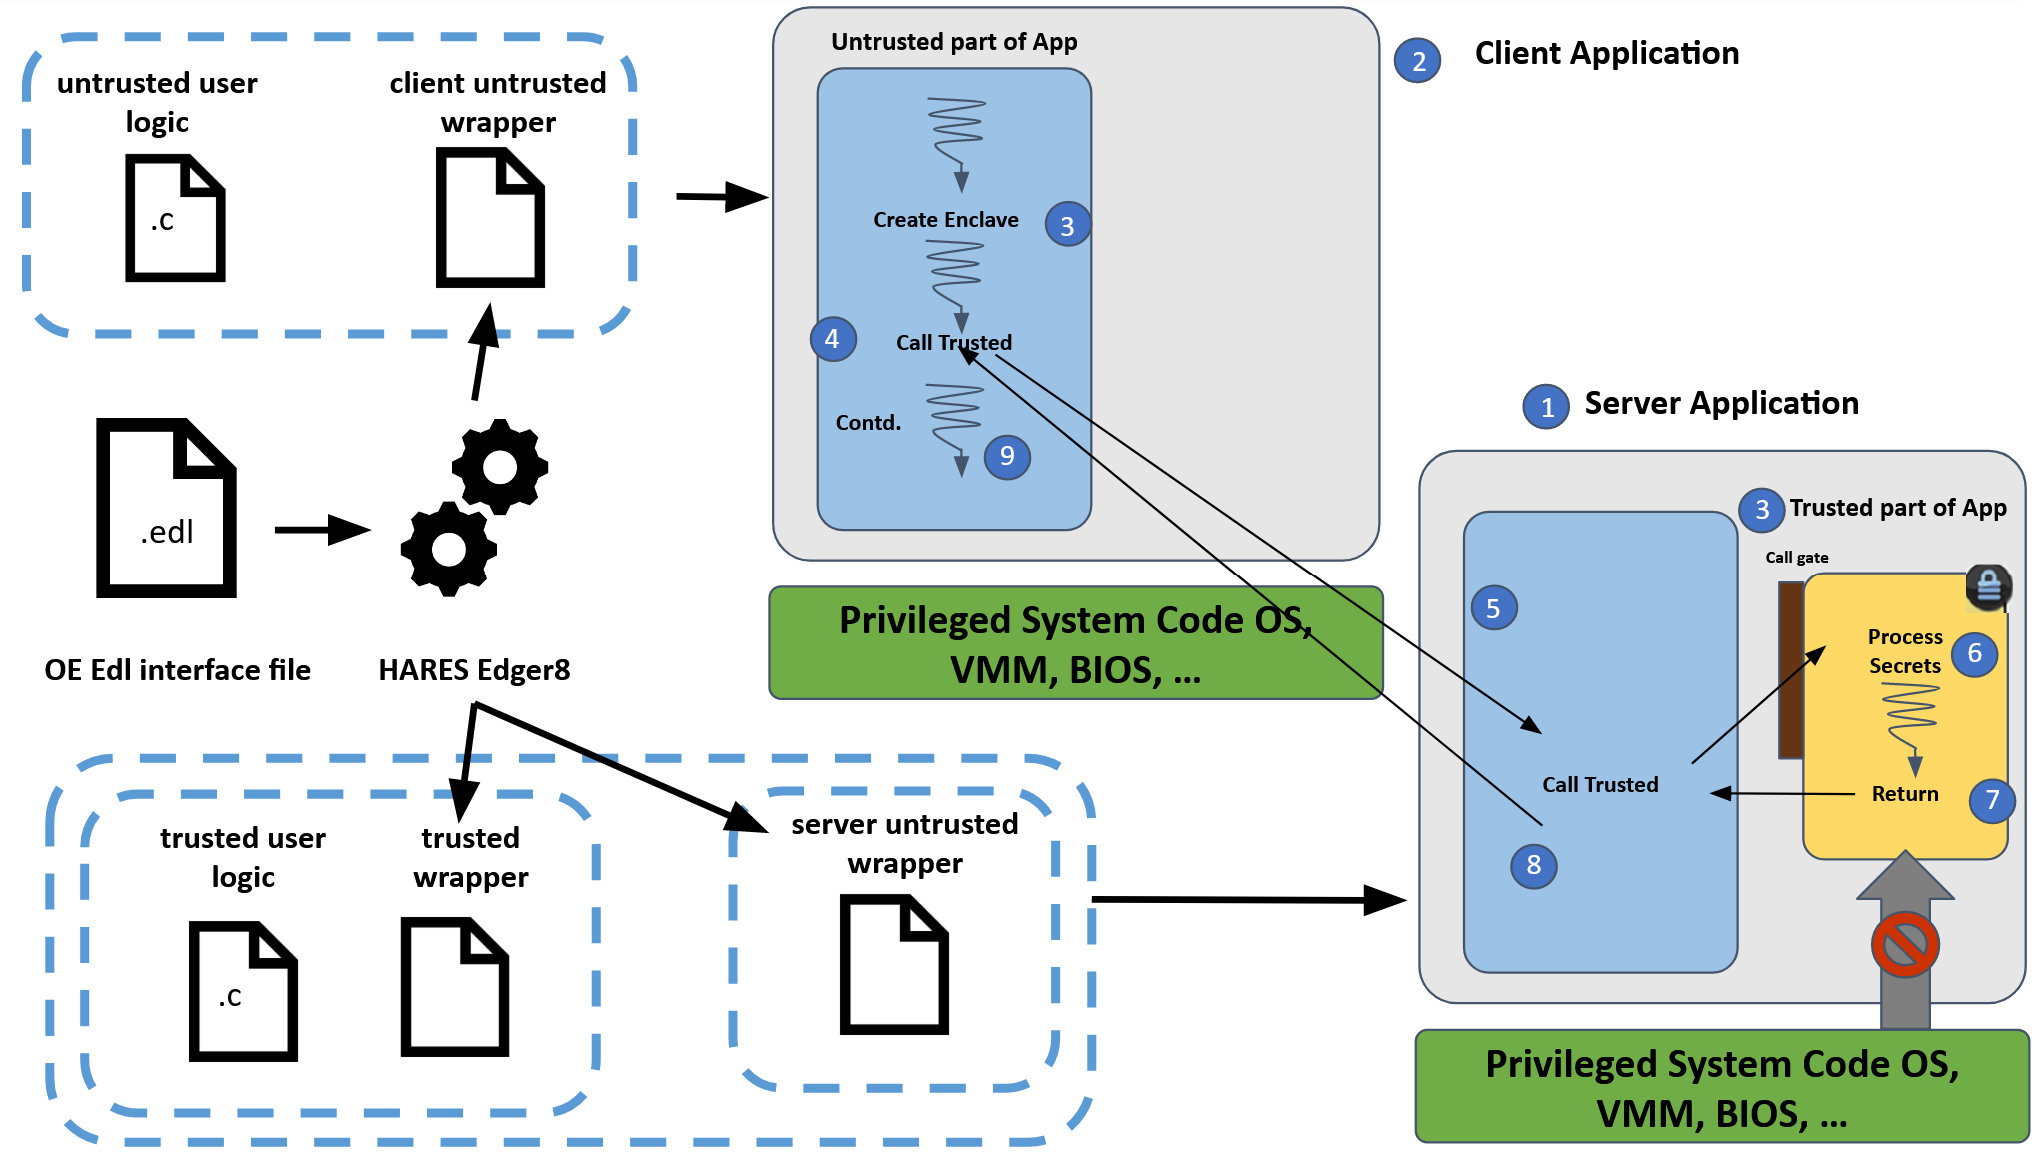
\includegraphics[scale=0.80]{figures/rpc_mode_arch.png}
            \caption{\monitor edger8 tool generating wrapper codes.} 
            \label{fig:HARES edger8 tool generating wrapper codes}
        \end{figure}
    }

    \subsection{Server and Client wrapper of \monitor RPC mode} \label{Server and client wrapper of RPC mode}
    
    The \monitor version of the \textsc{edger8r} tool, called \monitor \textsc{edger8r}, develops wrappers in a different way depending on whether the node is SGX capable or incapable. This is illustrated in Figure \ref{fig:HARES edger8 tool generating wrapper codes}. 
    
    On the server side, the wrapper created by the modified tool establishes a closed loop that involves generating and sending the reference of the enclave instance to the requester. It also manages the execution of valid enclave calls with pointer adjustment and readjustment, as discussed in Section \ref{adj_and_readj_of_monitor}. On the client side, all of the enclave function's definitions are replaced with TCP socket-based communication APIs that transmit the necessary information to the server side. 
    
    Figure \ref{fig:server_state_machine} shows the state machine of the \monitor wrapper code within the server side.

    \begin{figure}[htb]
        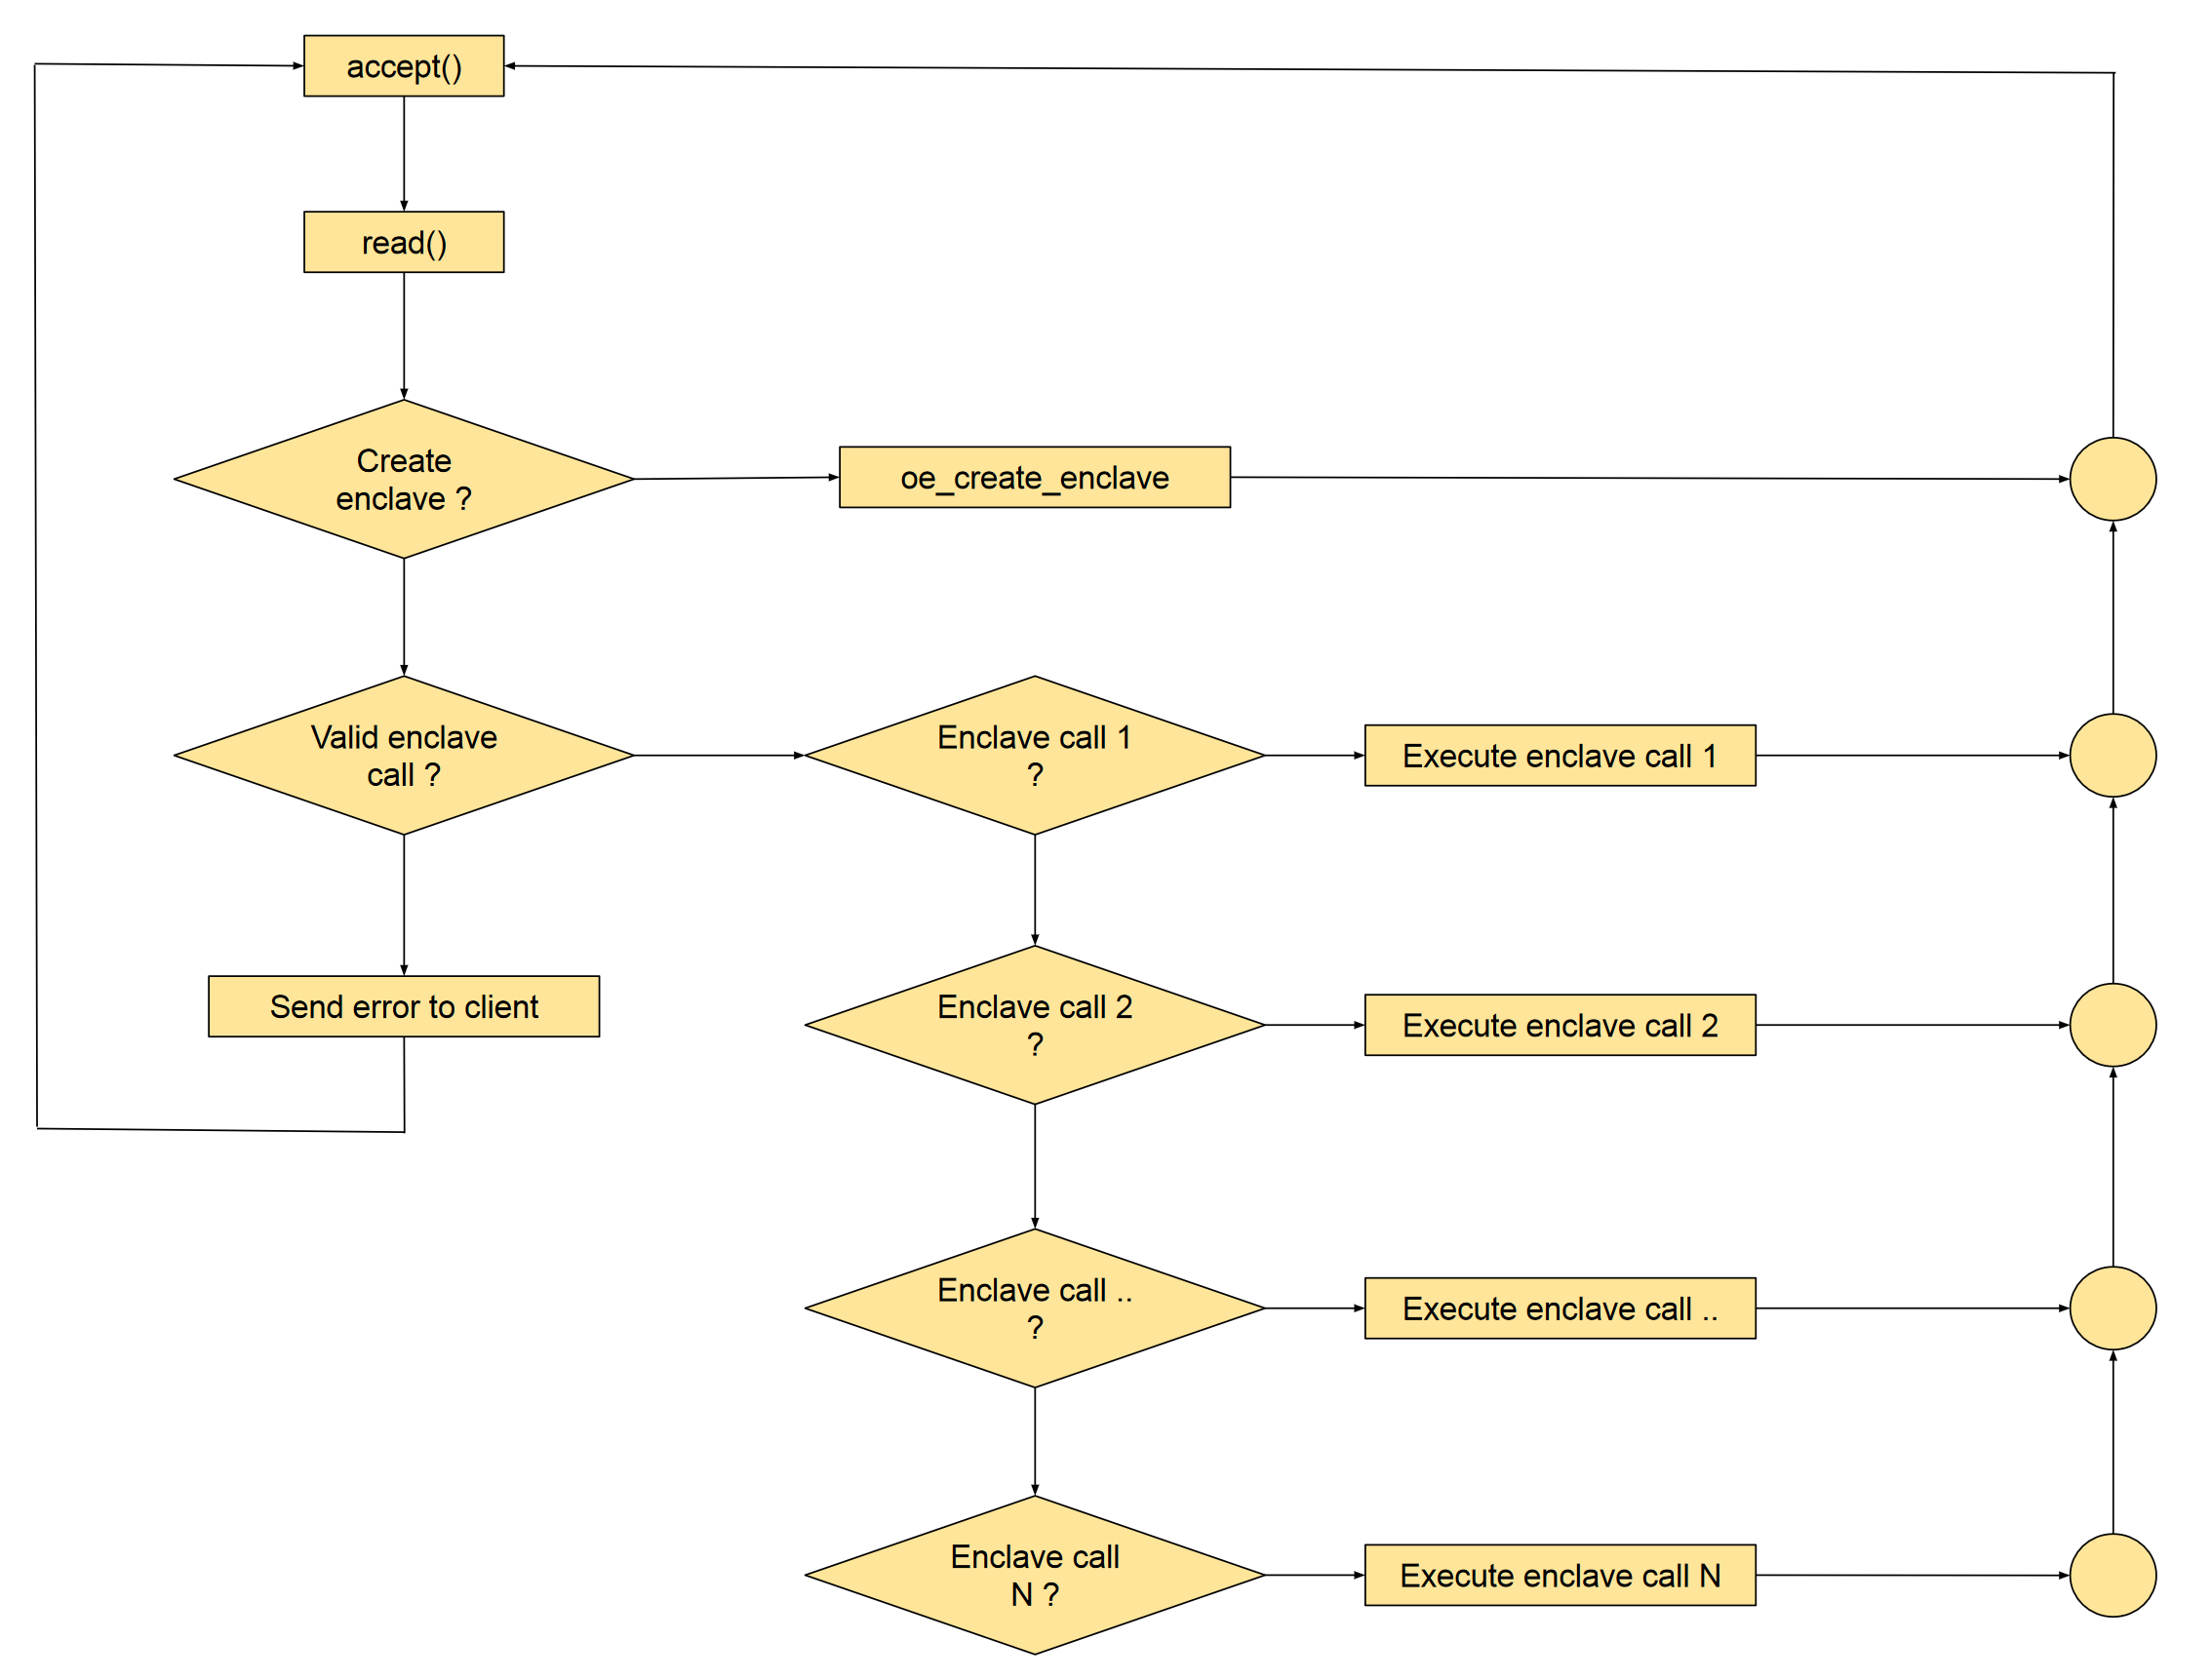
\includegraphics[scale=0.3]{figures/server_state_machine.png}
        \caption{State machine of the server.} 
        \label{fig:server_state_machine}
    \end{figure}
    
    Figure \ref{fig:HARES edger8 tool generating wrapper codes} illustrates the server application and the client application in the figure to give us a high-level idea of how the RPC mode of \monitor works. Initially, the untrusted part of the application residing on the non-SGX node executes as is until it wants to execute an enclave function. Once the execution reaches the create enclave function, the wrappers created by the \monitor edger8r send all the information needed to the wrappers residing on the other node, i.e., the SGX capable node. Here, the wrapper code calls the enclave function as it would be normally generated. After enclave execution, the control is transferred back to the non-SGX node with the client-side wrapper created by the edger8r tool. The afore-mentioned logic continues as long as an enclave function is to be executed until the end of application execution. 

    \chapter{Evaluation} \label{ch:Evaluation}
    This chapter is organized into the following sections. Section \ref{ase:experimental setup} introduces the experimental setup used for evaluating \monitor. Following that, Sections \ref{ase:Performance breakdown of remote enclave calls}, \ref{ase:performance evaluation of monitor mode}, \ref{sse:system_call_events_monitor_mode} delve into the performance evaluation of applications, providing a breakdown for the \monitor Monitor mode. Similarly, Sections \ref{sse:Performance evaluation of RPC mode}, \ref{sse:Profiling of serialization and deserialization cost for RPC mode} discuss the performance of \monitor RPC mode. Finally, Section \ref{sse:Security evaluation} conducts the security evaluation of \monitor.
    
    \section{Experimental setup} \label{ase:experimental setup}
    The evaluation setup consists of two machine nodes: an SGX-enabled machine and a non-SGX machine. For the non-SGX machine, we used Neoverse-N1 based Aarch64 machine and an Intel Xeon-based x86 machine for SGX heterogeneous offloading. On the other hand, for homogeneous offloading, we employed two Intel Xeon-based machines, one with SGX enabled and the other with SGX disabled. 

    \begin{table}[h]
	\centering
	\footnotesize
	\caption{Experimental hardware setup.}
	\begin{tabular}{| c | c | c | c |} \hline
		Scenarios & \multicolumn{2}{|c|}{Heterogeneous offloading} & Homogeneous offloading \\ \hline \hline
		CPU & \makecell{Neoverse-N1 \\(ARMv7)} & \makecell{Intel Xeon \\P-8370C} & \makecell{Intel Xeon \\CPU P-8370C} \\ \hline
		Cores & 2 & 2 & 2 \\ \hline
		Clock (GHz) & 2.3 GHz & 2.8 GHz & 2.8 GHz \\ \hline
		RAM & 8 GB & 16 GB & 16 GB \\ \hline
		Intel SGX & No & Yes & No \\ \hline
       Interconnect & \multicolumn{2}{|c|}{1 Gbps Ethernet} & 10 Gbps Infiniband \\ \hline
	\end{tabular}
	\label{t:setup}
    \end{table}
    
    \section{Performance breakdown of remote enclave calls for \monitor Monitor mode} \label{ase:Performance breakdown of remote enclave calls}
    The \monitor monitor mode uses several key mechanisms to transparently offload enclaves to an SGX-enabled machine, such as the ptrace APIs, the userspace page fault handling, and the CRIU's compel framework for extending virtual memory ranges, to name a few. Understanding these components interplay is essential to identify potential bottlenecks and better optimize \monitor. We inserted timestamps in the \monitor debug mode and printed the time consumed by each \monitor component into a log file. As reported in Table \ref{t:TimeConsumingCalls}, most \monitor internal API calls consume less than 50 us. There are two outliers: the compel API for injecting parasite code into the running program and the ptrace interface for page read/write operations, consuming 0.5 ms and 0.75 ms, respectively.

    The compel APIs (whether to steal the userfaultfd descriptor from the target or to extend the target’s virtual memory) take around 0.5 ms to complete. This latency can be attributed to the number of tasks needed to infect the victim process with the parasitic code, such as stopping the victim process, preparing the infection handler, executing the remote code, curing the victim, and finally, resuming the victim process. Fortunately, we don’t need to frequently invoke compel once the target process is launched. The ptrace system call, especially for memory page read/write, also has a high overall latency of approximately 0.75 ms per page (where each page is 4096 bytes). This increased latency can be attributed to various factors, including system call overhead and data movement. Interestingly, transferring pages across nodes took less time than PTRACE\_PEEKDATA/PTRACE\_POKEDATA.

    \begin{table*}[t]
    \centering
    \footnotesize
    \caption{Execution time breakdown of \monitor APIs in the cloud setting.}
    \begin{tabular}{| c | c |} \hline
          API & Average time taken \\ \hline \hline
        \textbf{Compel APIs}  &  \textbf{0.5 ms}\\ \hline
        UFFD APIs &  12 us \\ \hline
        PTRACE\_GETREGS | PTRACE\_SETREGS API  &  10 us\\  \hline
        PTRACE\_POKETEXT | PTRACE\_PEEKTEXT API & 6 us\\ \hline
        \textbf{PTRACE\_PEEKDATA | PTRACE\_POKEDATA API (per page)} & \textbf{0.75 ms} \\ \hline 
        REMOTE\_EXECUTE & 2 us \\ \hline
        VMA\_FROM\_REMOTE & 4 us \\ \hline
        VMA\_BUFFER\_HEADER & 20 us \\ \hline
        VMA\_BUFFER & 50 us \\ \hline
        VMA\_TRANS\_ACK & 10 us \\ \hline
        REMOTE\_REGS & 20 us \\ \hline
    \end{tabular}
    \label{t:TimeConsumingCalls}
    \end{table*}
    
    \section{Performance evaluation of Monitor mode} \label{ase:performance evaluation of monitor mode}
    We conducted comprehensive tests to evaluate the performance overhead of monitor mode on various applications. Our tests included SGX-DNet (an Intel SGX version of the Darknet machine learning library), Plinius (a secure machine learning framework that uses Intel SGX for secure training of neural network models and persistent memory for fault tolerance), two memory intensive benchmarks – bw\_mem and lat\_read (from an SGX ported lmbench) and a file encryptor, a data sealing applications from the Open Enclave SDK. We present the normalized results of offloading the enclave from a docker instance running on a non-SGX machine to an SGX-enabled machine node, with a baseline of running the vanilla enclave on an SGX-enabled docker instance alone. Figure \ref{fig:normalized_perf}  shows the normalized result. We also reported the total execution time in Table.\ref{tab:exe_time}.

    \begin{table*}[t]
    \caption{Application Execution Time with \monitor Monitor mode.}
    \footnotesize
    \centering
    \begin{tabular}{|l|l|l|l|l|l|l|}
        \hline
        Application mode & SGX\_DNet & Plinius & bw-mem & lat-read & File\_Encryptor & Data\_Sealing \\ \hline
        Native Execution   & 116 s & 166 s   & 40153 ms & 46034 ms & 431 ms  & 450 ms      \\ \hline
        Enclave Offloading & 122 s & 168 s   & 40692 ms & 46597 ms & 1686 ms & 4986 ms     \\ \hline
    \end{tabular}
    \label{tab:exe_time}
    \end{table*}

    For applications with longer execution time (e.g., SGX-DNet and Plinius), \monitor does not bring significant performance overhead. For small applications with shorter execution time, the remote enclave offloading and control flow transformation cost dominate the overall execution time. Thus, applications such as file encryptor and data sealing have a larger normalized performance overhead. 

        \begin{figure}[htb]
            \centering
            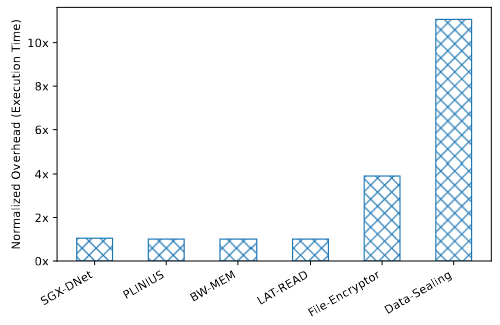
\includegraphics[scale=2.5]{figures/Normalized_performance.png}
            \caption{ Normalized performance overhead of running offloaded enclave applications using \monitor monitor mode against local execution in the cloud setting.} 
            \label{fig:normalized_perf}
        \end{figure}

    \section{Profiling of number of system events for Monitor mode} \label{sse:system_call_events_monitor_mode}
    To better explain the performance overhead that varies among different benchmarks, we further measured several other metrics, such as the number of enclave calls executed, synchronization messages used, pages transferred, injected parasite code calls, and the number of ptrace calls during the evaluation process. Figure \ref{fig:client_instructions} illustrates the results.

    \begin{figure}[H]
    \centering
    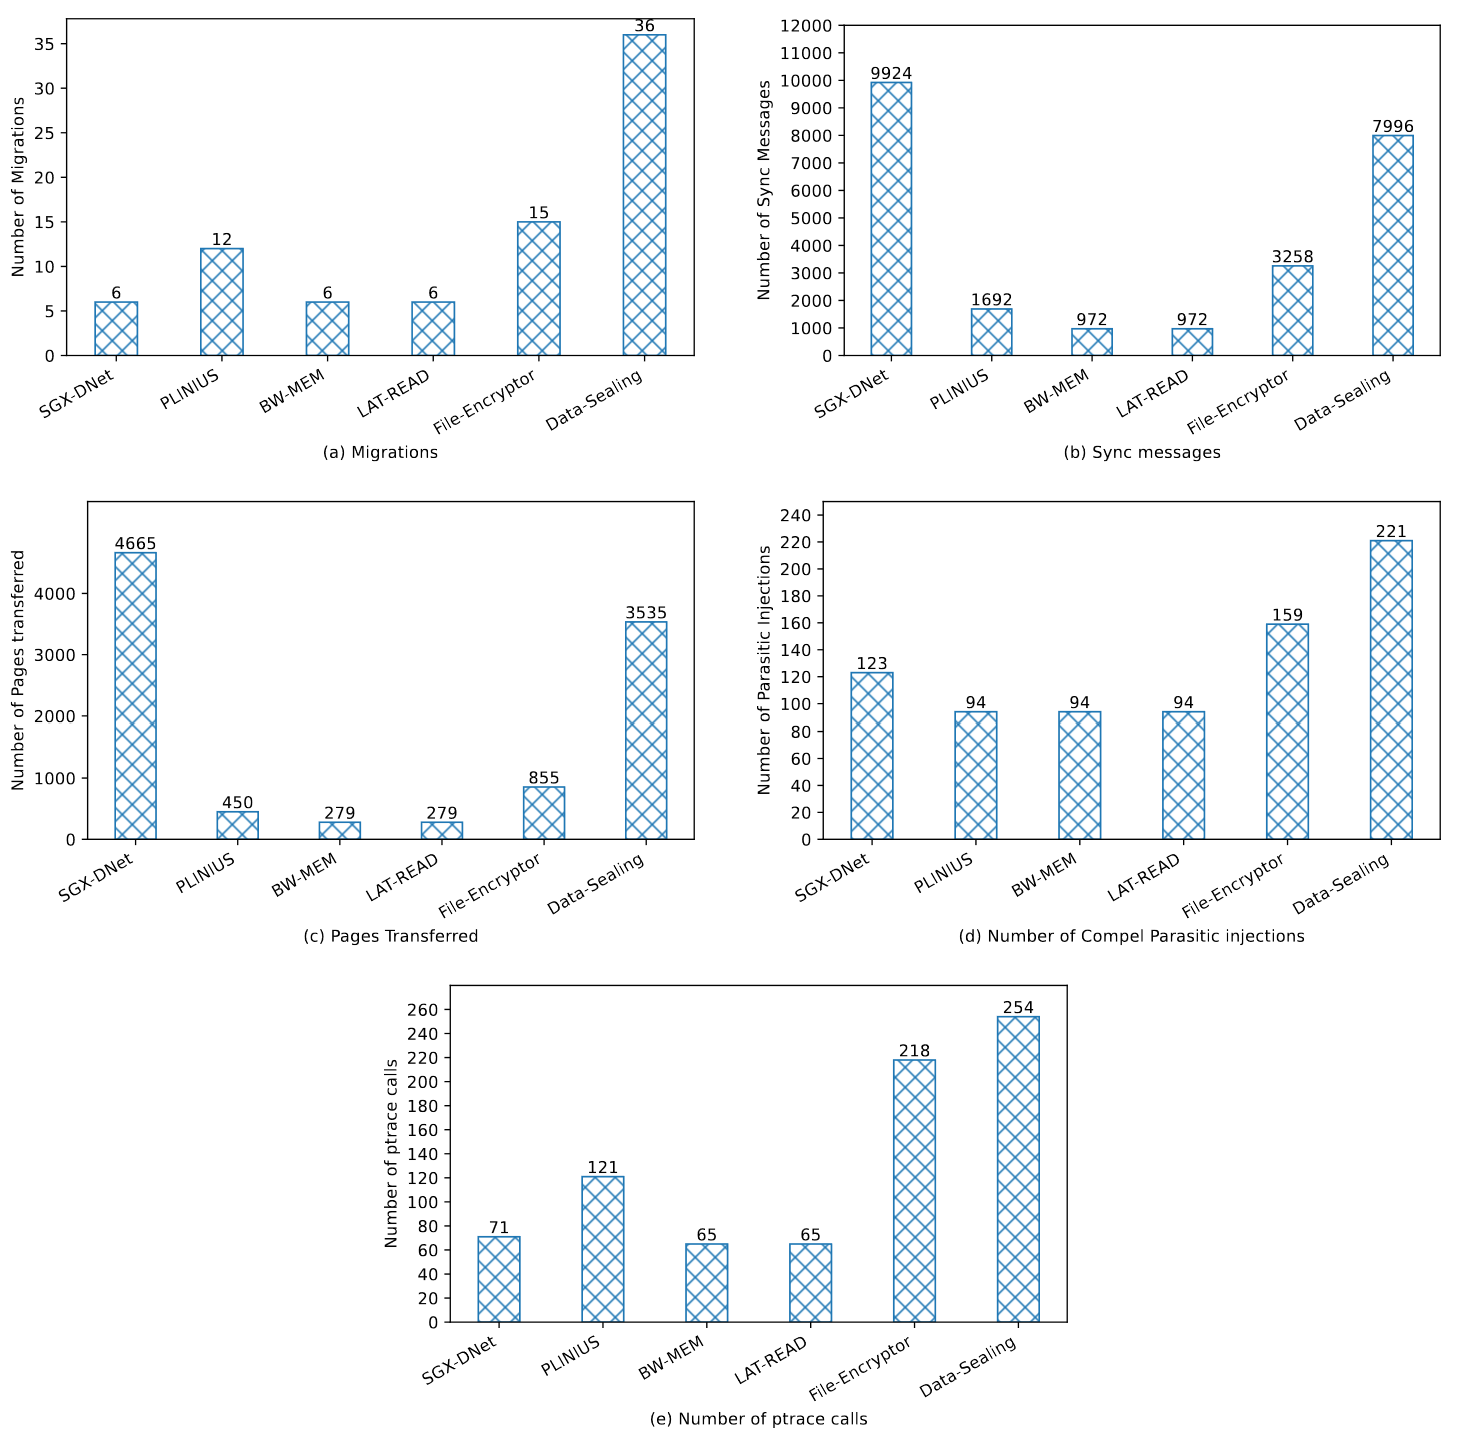
\includegraphics[scale=1.1]{figures/perf_char_monitor.png}
    \caption{Profile of a number of system events while running applications with monitor mode.} 
    \label{fig:client_instructions}
    \end{figure}

    As one can see from Figure (a) of \ref{fig:client_instructions}, the number of migrations is higher for applications such as File-encryptor and Data-Sealing. Additionally, along with the migrations, the number of pages that often change is also higher with File-encryptor and Data-sealing applications. This leads to an increase in the number of compel parasitic injections and a higher number of ptrace calls, resulting in larger overhead for those applications.
    
    \section{Performance evaluation of RPC mode} \label{sse:Performance evaluation of RPC mode}
        \begin{figure}[htb]
            \centering
            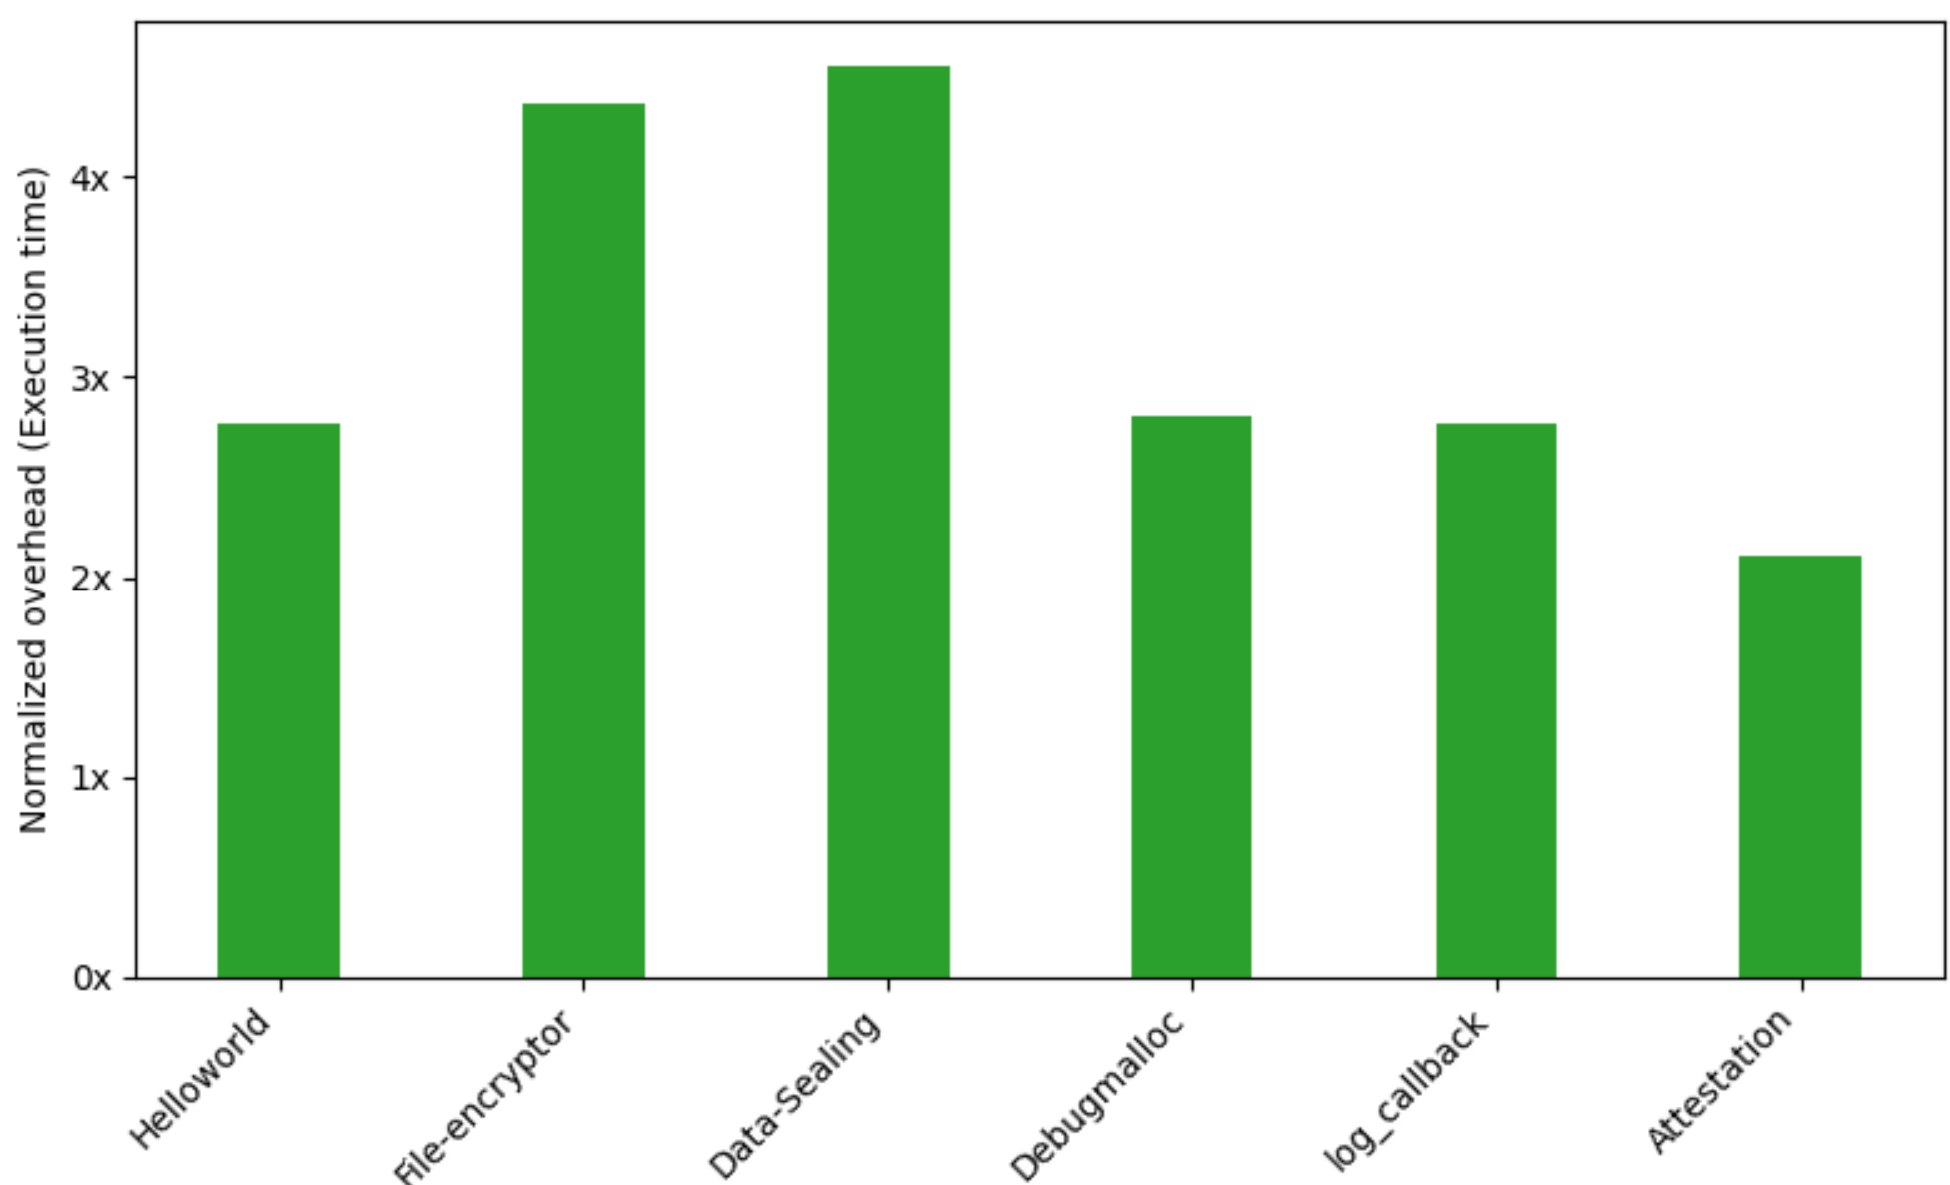
\includegraphics[scale=0.7]{figures/Normalized_performance_rpc.png}
            \caption{Normalized performance overhead of running heterogeneous offloaded enclave applications using \monitor RPC mode against local execution in the cloud setting.} 
            \label{fig:rpc_enclave_offloading}
        \end{figure}

    For evaluating the \monitor RPC mode, we used some of the applications that come along with the Open Enclave SDK and the results are shown in Figure. \ref{fig:rpc_enclave_offloading}. Although comparing the performance of heterogeneous offloading to homogeneous offloading is an apples-to-oranges comparison, as we have a weaker non-SGX machine for heterogeneous offloading (Neoverse-N1) and the network bandwidth is also slower in heterogeneous offloading with just a 1-Gigabyte bandwidth. \monitor's RPC based heterogeneous offloading despite being less powerful and slower networking speed, the performance overhead is relatively lower compared to the overhead of the \monitor Monitor mode. As one can see with File-encryptor whose normalized performance was comparable with homogeneous offloading and at times better with some applications like Data-sealing. This is mainly because the RPC mode of \monitor avoids time-taking APIs such as compel's parasitic injection, PTRACE, and mainly the page synchronization.
    
    
    \section{Profiling of serialization and deserialization cost for RPC mode} \label{sse:Profiling of serialization and deserialization cost for RPC mode}
    Similar to the profiling of the APIs for the \monitor Monitor mode in Section \ref{sse:system_call_events_monitor_mode}, this section breaks down the performance results for Figure \ref{fig:rpc_enclave_offloading}. The results are shown in Figures \ref{fig:perf_breakdown_rpc} and \ref{fig:profile_rpc}. Networking performance significantly impacts the overall performance of the application, with a considerable amount of time being spent on transferring bytes back and forth. Another interesting observation is that serialization or deserialization takes very minimal time, in fact, just a few milliseconds.

    \begin{figure}[htb]
        \centering
        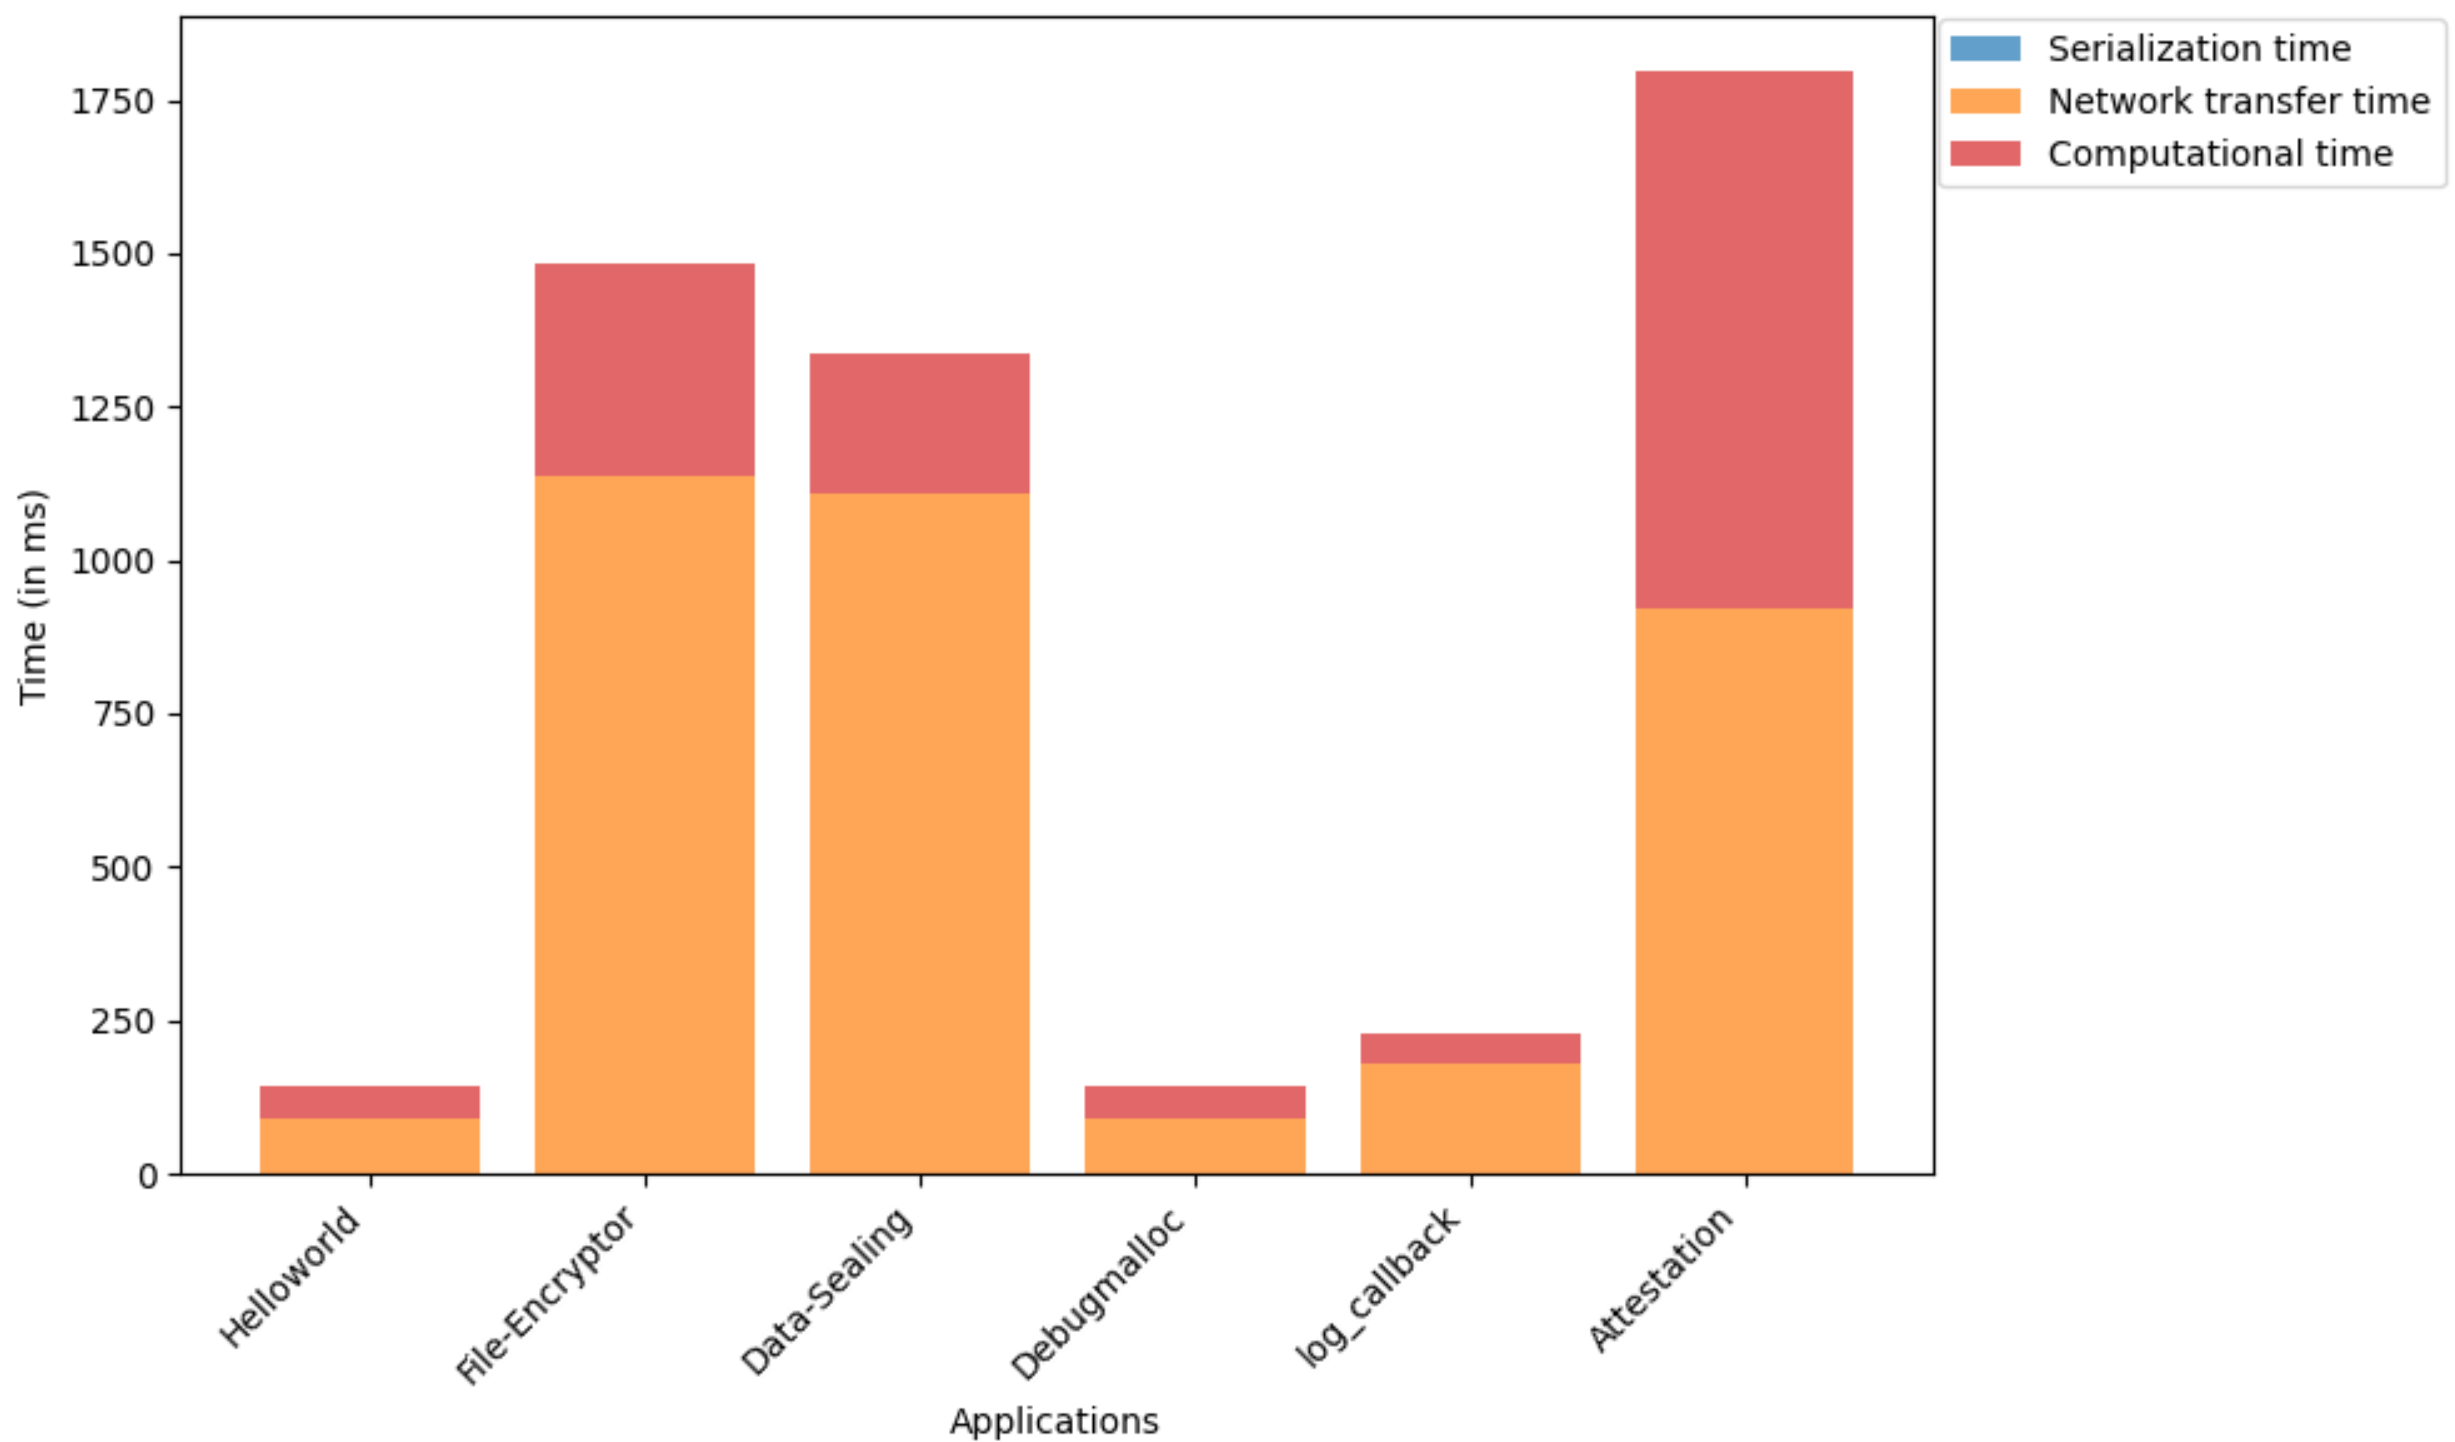
\includegraphics[scale=0.6]{figures/perf_breakdown_rpc.png}
        \caption{Performance Characterization of Applications with \monitor RPC Mode.} 
        \label{fig:perf_breakdown_rpc}
    \end{figure}

    \begin{figure*}[htp]
    \centering
    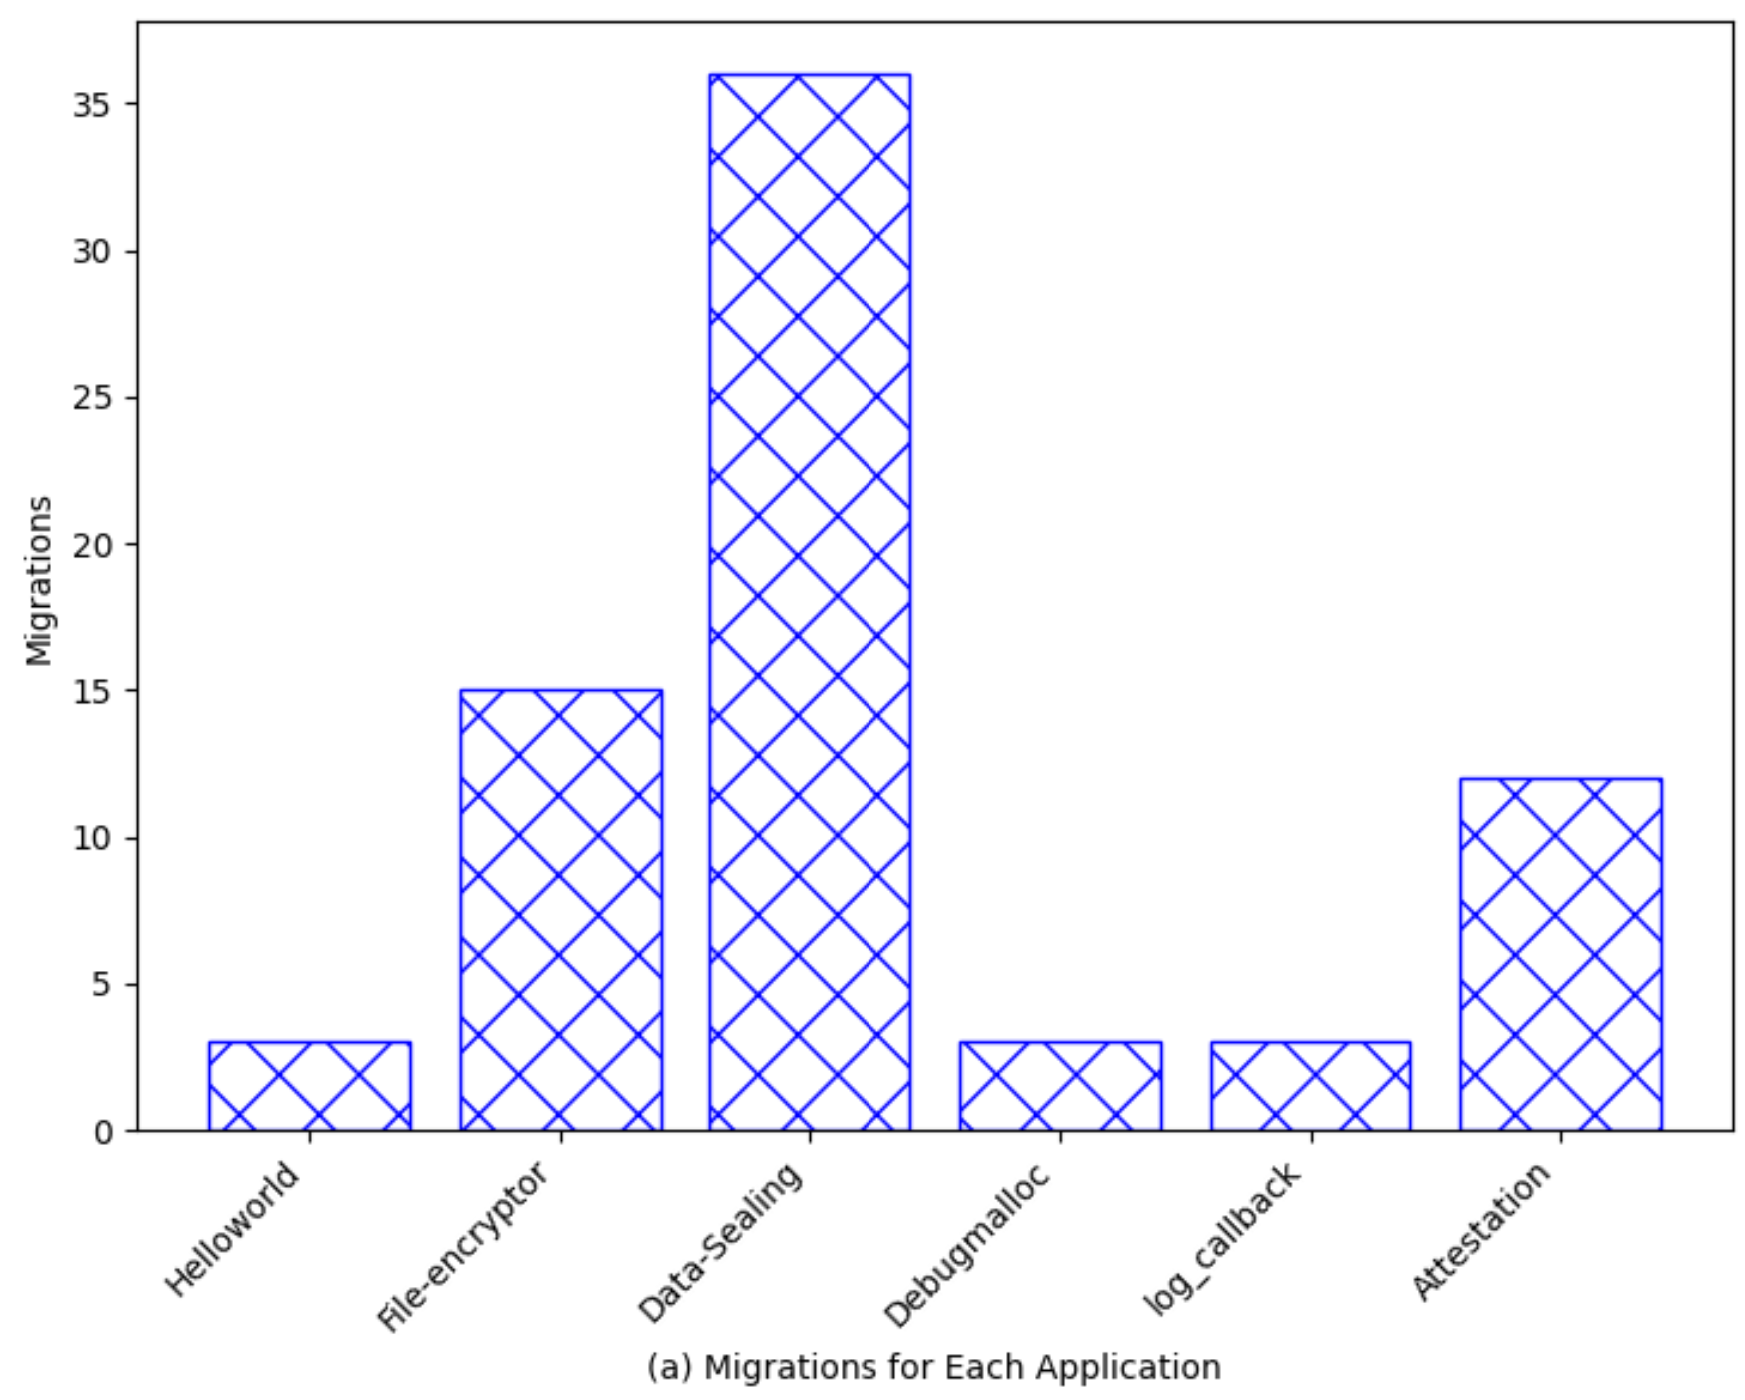
\includegraphics[width=.50\textwidth]{figures/a-migrations_rpc.png}%
    \hfill
    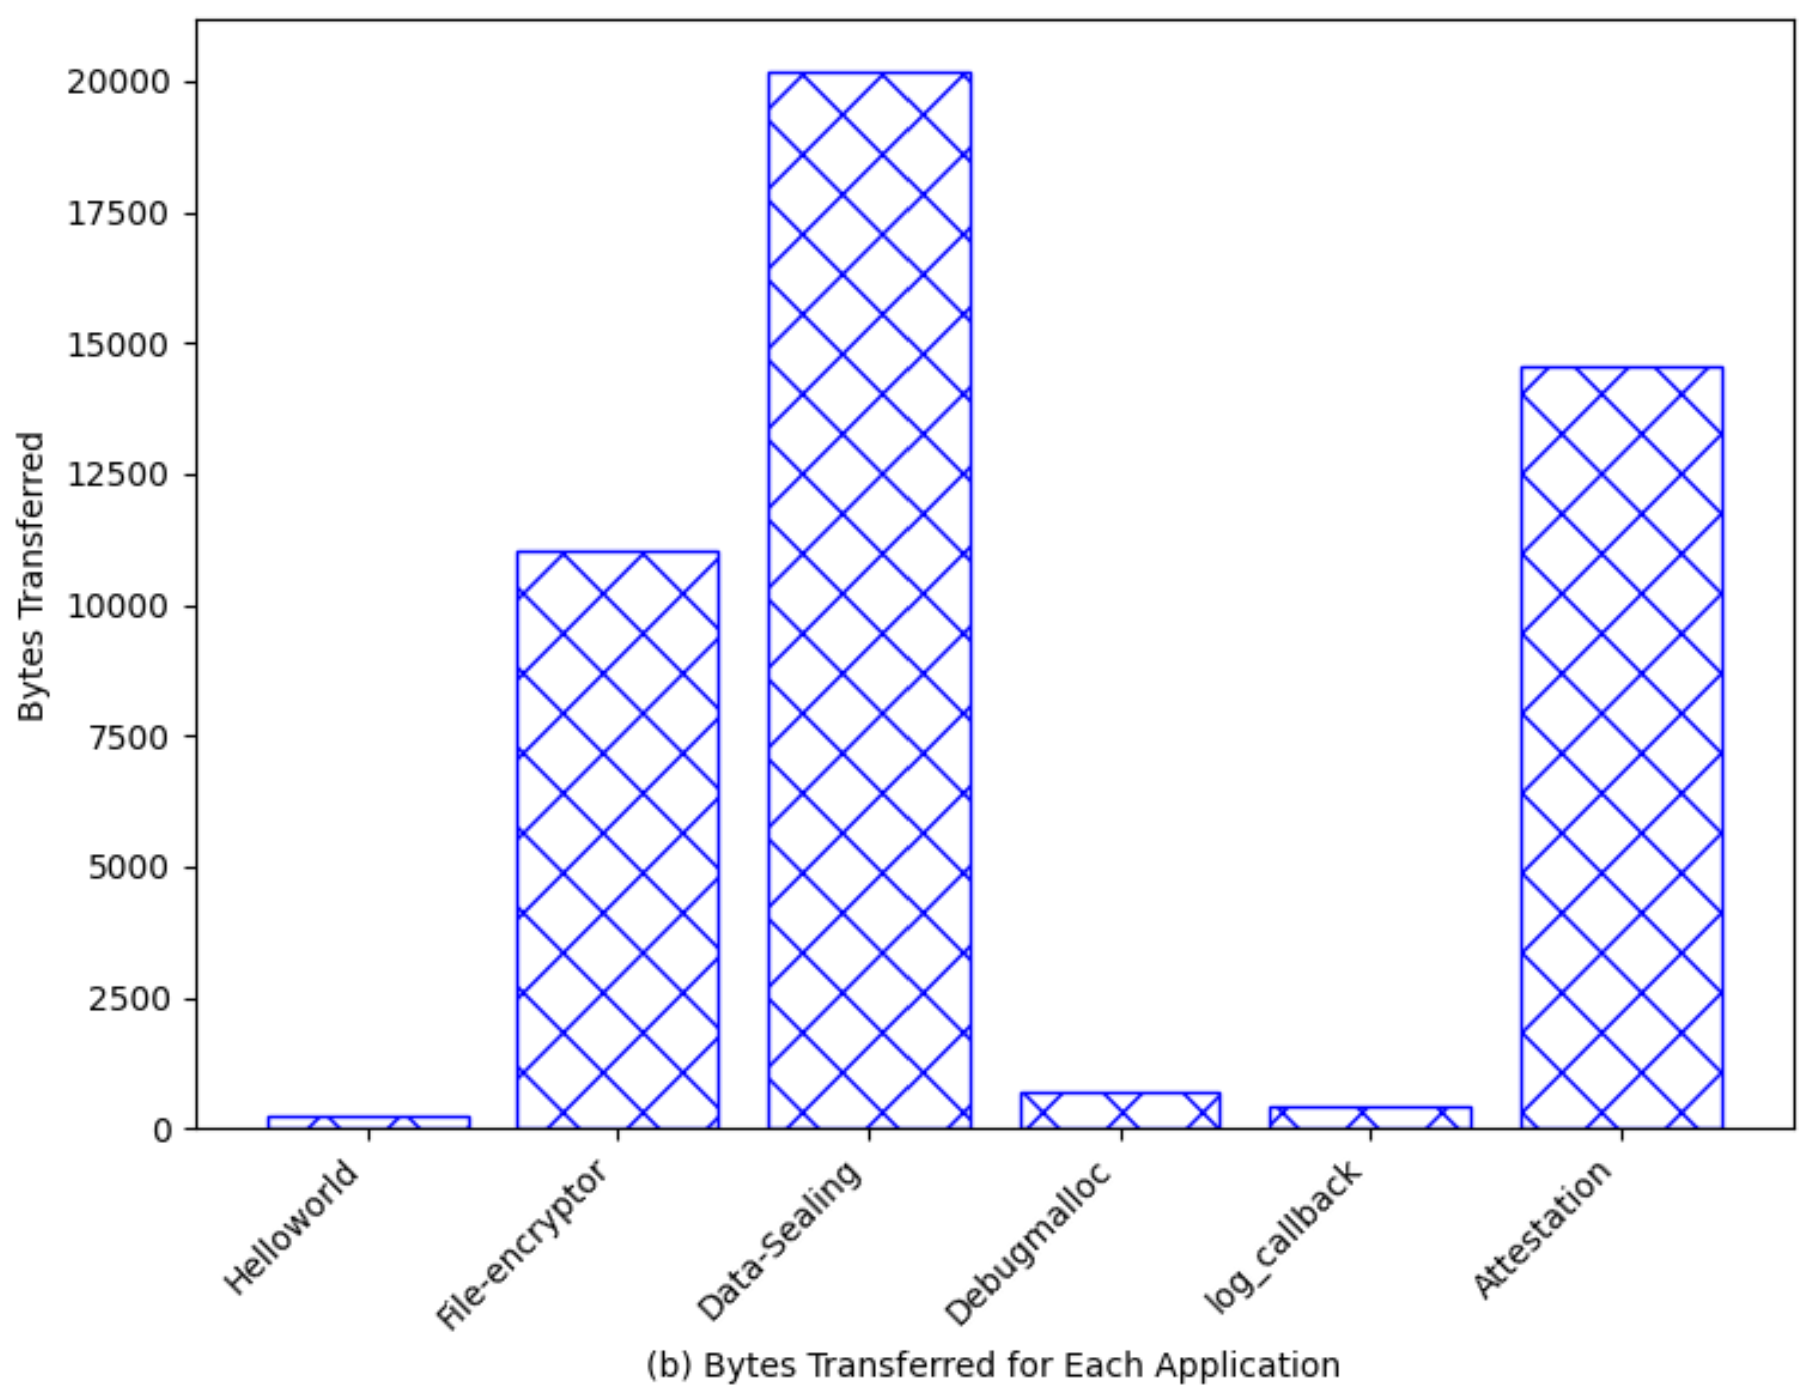
\includegraphics[width=.50\textwidth]{figures/b-bytes_transferred_rpc.png}%
    \caption{Profile of a number of system events while running applications with RPC mode.}
    \label{fig:profile_rpc}
    \end{figure*}

    
    \section{Security evaluation} \label{sse:Security evaluation}
    The primary objective of \monitor is to address the security hardware availability gap in both homogeneous and heterogeneous environments. This section focuses on the security evaluation of \monitor and is structured as follows. Subsection \ref{ase:threat model} outlines the threat model for \monitor. Following that, subsection \ref{cve analysis} conducts an analysis of Common Vulnerabilities and Exposures (CVE) for \monitor. Finally, subsection \ref{remote attestation} explores the remote attestation capability of \monitor. 
    
    \subsection{Threat model} \label{ase:threat model}
    We assume a threat model that falls in line with the threat model of SGX. The adversary is believed to be in possession of super root privileges who has access to all the software and physical hardware. Hence, all the software including the instances of \monitor, Untrusted part of \monitor client, Operating System along with the hardware such as DRAM, other peripherals across two nodes are not trusted. We solely rely upon the SGX based CPU along with the enclave and trust the primitives of Intel SGX mechanism.

    Furthermore, we assume that the code running inside enclave is benign and does not voluntarily relinquish any secret keys or critical information. Enclave developers are expected to implement security techniques, such as the one discussed in \cite{Protecting, SGX-Defense}, to safeguard against potential vulnerabilities in the enclave binary interface. Additionally, we take no responsibility in addressing the side channel attacks upon SGX enclaves. With our system, known as \monitor, when an enclave is offloaded onto a remote node, it inherits the standard security benefits provided by the standard SGX protection mechanisms. This ensures that sensitive operations within the enclave remain secure and isolated from potential threats.

    \subsection{CVE analysis} \label{cve analysis}
    In this section, we will enumerate and comprehensively discuss the types of CVEs that can be protected by leveraging the SGX as offered by \monitor. The \monitor plays a pivotal role in mitigating prevalent weaknesses and vulnerabilities, such as CWE-798 (Use of Hard-coded Credentials), CWE-200 (Information Exposure), CWE-321 (Hardcoded Cryptographic Key), CWE-326 (Inadequate Encryption Strength), and numerous others. Sadly, these kinds of vulnerabilities still persist within the realm of IoT, yet they can be readily averted through the utilization of SGX, as offered by \monitor. The Table \ref{t:CVEs} lists some of the CVEs that could be mitigated by deploying \monitor.

    For example, CVE-2019-13604 represents a vulnerability arising from a short key weakness, enabling potential attackers to employ brute force techniques to extract the key used for image obfuscation, subsequently granting them access to decrypt the protected image. With \monitor, the encryption key can be initially generated within the enclave and securely sealed in protected storage for future encryption \& decryption of images. In this case, even if an attacker manages to compromise the host system, they will be unable to access the enclave or extract the encryption key, rendering the brute force attack ineffective. Similarly, consider CVE-2023-37468, where passwords are stored in clear text within the database, devoid of encryption. This vulnerability can also be averted by utilizing \monitor SGX to encrypt the passwords along with the database using the SGX based SQLite alike databases that \monitor support, thereby enhancing their security.

    Another commonly encountered attack is the Return-Oriented Programming (ROP) attack \cite{Remote-procedure-call}. In this type of attack, the attacker adeptly manipulates the stack, exploiting buffer overflow vulnerabilities in the program to execute arbitrary code. Notably, successful ROP attacks often require knowledge of the state of registers and memory addresses. However, SGX offers protection by encrypting the entire memory contents of the enclave program along with an additional feature of providing encrypted enclave code. This will thwart the buffer overflow vulnerabilities from exploiting the arbitrary code execution on enclave code unless specified through the allowed Ecall entries. Furthermore, It's important to note that while SGX itself can be vulnerable to ROP-based attacks stemming from memory corruption vulnerabilities within the code residing in an enclave as illustrated by \cite{ROP-paper}, our focus here is specifically on addressing the protection mechanisms of the \monitor enclave against memory vulnerabilities originating from untrusted code. This approach enables the prevention of CVEs such as CVE-2017-10720 and CVE-2023-25668.

    \begin{table*}[t]
    \centering
    \footnotesize
    \caption{CVEs that could be mitigated with \monitor.}
    \begin{tabular}{| c | c |} \hline
          CWE & CVE \\ \hline \hline
        Buffer overflows & CVE-2017-10720, CVE-2017-10722, CVE-2023-25668\\ \hline  
        Hardcoded Credentials & CVE-2021-33220, CVE-2023-37468, CVE-2021-33219\\ \hline
        Information exposure & CVE-2019-0741 \\ \hline
        Hardcoded crytographic keys & CVE-2015-4080 \\ \hline
        Inadequate encryption strength & CVE-2019-13604, CVE-2019-13603 \\ \hline
    \end{tabular}
    \label{t:CVEs}
    \end{table*}

    \subsection{Remote Attestation} \label{remote attestation}
    With the utilization of \monitor, remote attestation functions in a manner similar to other use cases. Initially, the host process, residing in the non-SGX node, receives the challenge from the remote attestation service. This challenge is subsequently decrypted and signed by the enclave in the SGX node, facilitated by the \monitor. Following the completion of enclave’s operation, the enclave report, along with the signature from the quoting enclave will be sent to the remote attestation service from the host process in non-SGX node. Finally, the host process in the non-SGX receives the verification report from the remote attestation service.

    \chapter{Conclusion} \label{ch:conclusion}
    \section{Summary of Contributions}
    In this thesis, we introduced \monitor, a system designed to offload confidential computation across homogeneous and heterogeneous boundaries. Embedded and other resource-constrained systems often lack sophisticated security measures, such as Trusted Execution Environment (TEE), making them suitable candidates for leveraging the capabilities of \monitor. The system incorporates a memory synchronization model facilitated by a userspace monitor for framework-agnostic homogeneous offloading. Additionally, it employs an RPC-based design for Open Enclave-based heterogeneous offloading.
    
    To offload computations to a remote node, both modes of \monitor exhibit a significant dependency on networking. Therefore, with faster networks, \monitor, regardless of its mode, will deliver better performance for offloading confidential computation.
    
    The major contributions of \monitor can be summarized as follows:
    \begin{enumerate}
        \item We implemented two modes of \monitor, monitor and RPC, that allow programs to offload their hardware security extensions transparently across homogeneous and heterogeneous architectures. 
        \item We evaluated the prototype of \monitor using open-source machine learning and data sealing applications. With the evaluation results, we can observe that \monitor secures confidential computations on top of hybrid and distributed machines with an acceptable performance overhead.
        \item We conducted a security evaluation by identifying and addressing Common Vulnerability Exposures (CVE). This analysis underscores the advantages of utilizing \monitor to leverage remote Trusted Execution Environments (TEEs) as a means to mitigate and avoid such CVEs.
    \end{enumerate}

    The following section talks about the limitations of using \monitor and also about the future works to improve \monitor.

    \section{Limitations}
    Some of the limitations of \monitor are discussed in this section. 
    
    \begin{enumerate}
        \item In the monitor mode of \monitor, to offload confidential computations, the process's memory is duplicated on both nodes. While the confidential computations within the enclave remain secure, the duplication of the process's untrusted memory expands the attack surface. This expansion can cause potential security risks to untrusted computations.
        \item The \monitor presented in this thesis currently does not support multi-threading. While the incorporation of multi-threading is not infeasible, it would require engineering effort. The implementation would involve synchronizing all threads and placing them in a suspended state before migration. It's important to note that such an addition might introduce additional overhead to the overall performance.
        \item As mentioned in the Chapter \ref{ch:Evaluation}, the performance of \monitor primarily relies on network performance. This is particularly evident in the monitor mode of \monitor, where a substantial number of pages are transmitted back and forth during migrations for memory synchronization.
        \item Since \monitor is implemented solely in user-space, offloading secured computations that handle resources such as files and devices interchangeably across the trusted and untrusted worlds presents a challenge. This is due to the necessity for implementations to share resources within kernels residing across two nodes.
    \end{enumerate}
    
    \section{Future Work}
    This section discusses about the work that could expand the applications and efficiency of \monitor.

    In addition to Intel SGX's enclave, several other hardware security extensions can be considered for offloading. These extensions include pointer authentication \cite{pointer_authentication}, hardware-based control flow enhancement \cite{intel_cet}, memory tagging \cite{arm_mte}, and various others. Determining the scope and methodology for offloading these extensions represents an intriguing avenue for future research.

    Currenly for the monitor mode, supporting Address Space Layout Randomization (ASLR) \cite{ASLR} is also important, as it provides a security technique to prevent memory-based attacks on the system. This can be implemented by mapping the memory layout of one node onto the other and then updating the respective memory during the transition process.

    
	% This is the standard bibtex file. Do not include the .bib extension in <bib_file_name>.
	% Uncomment the following lines to include your bibliography: 
	%\bibliography{<bib_file_name>}
	%\bibliographystyle{plainnat}   
 
    \bibliographystyle{plainurl}
    \bibliography{references}

\end{document}

%****************************************************************************
% Below are some general suggestions for writing your dissertation:
%
% 1. Label everything with a meaningful prefix so that you
%    can refer back to sections, tables, figures, equations, etc.
%    Usage \label{<prefix>:<label_name>} where some suggested
%    prefixes are:
%			ch: Chapter
%     		se: Section
%     		ss: Subsection
%     		sss: Sub-subsection
%			app: Appendix
%     		ase: Appendix section
%     		tab: Tables
%     		fig: Figures
%     		sfig: Sub-figures
%     		eq: Equations
%
% 2. The VTthesis class provides for natbib citations. You should upload
%	 one or more *.bib bibtex files. Suppose you have two bib files: some_refs.bib and 
%    other_refs.bib.  Then your bibliography line to include them
%    will be:
%      \bibliography{some_refs, other_refs}
%    where multiple files are separated by commas. In the body of 
%    your work, you can cite your references using natbib citations.
%    Examples:
%      Citation                     Output
%      -------------------------------------------------------
%      \cite{doe_title_2016}        [18]
%      \citet{doe_title_2016}       Doe et al. [18]
%      \citet*{doe_title_2016}      Doe, Jones, and Smith [18]
%
%    For a complete list of options, see
%      https://www.ctan.org/pkg/natbib?lang=en
%
% 3. Here is a sample table. Notice that the caption is centered at the top. Also
%    notice that we use booktabs formatting. You should not use vertical lines
%    in your tables.
% 
%				\begin{table}[htb]
%					\centering
%					\caption{Approximate computation times in hh:mm:ss for full order 						versus reduced order models.}
%					\begin{tabular}{ccc}
%						\toprule
%						& \multicolumn{2}{c}{Computation Time}\\
%						\cmidrule(r){2-3}
%						$\overline{U}_{in}$ m/s & Full Model & ROM \\
%						\midrule
%						0.90 & 2:00:00 & 2:08:00\\
%						0.88 & 2:00:00 & 0:00:03\\
%						0.92 & 2:00:00 & 0:00:03\\
%						\midrule
%						Total & 6:00:00 & 2:08:06\\
%						\bottomrule
%					\end{tabular}
%					\label{tab:time_rom}
%				\end{table}
% 
% 4. Below are some sample figures. Notice the caption is centered below the
%    figure.
%    a. Single centered figure:
%					\begin{figure}[htb]
%						\centering
%						\includegraphics[scale=0.5]{my_figure.eps}
%						\caption{Average outlet velocity magnitude given an average  
%				        input velocity magnitude of 0.88 m/s.} 
%						\label{fig:output_rom}
%					\end{figure}
%    b. Two by two grid of figures with subcaptions
%					\begin{figure}[htb]
%						\centering
%						\begin{subfigure}[h]{0.45\textwidth}
%							\centering
%							\includegraphics[scale=0.4]{figure_1_1.eps}
%							\caption{Subcaption number one}
%							\label{sfig:first_subfig}
%						\end{subfigure}
%						\begin{subfigure}[h]{0.45\textwidth}
%							\centering
%							\includegraphics[scale=0.4]{figure_1_2.png}
%							\caption{Subcaption number two}
%							\label{sfig:second_subfig}
%						\end{subfigure}
%
%						\begin{subfigure}[h]{0.45\textwidth}
%							\centering
%							\includegraphics[scale=0.4]{figure_2_1.pdf}
%							\caption{Subcaption number three}
%							\label{sfig:third_subfig}
%						\end{subfigure}
%						\begin{subfigure}[h]{0.45\textwidth}
%							\centering
%							\includegraphics[scale=0.4]{figure_2_2.eps}
%							\caption{Subcaption number four}
%							\label{sfig:fourth_subfig}
%						\end{subfigure}
%						\caption{Here is my main caption describing the relationship between the 4 subimages}
%						\label{fig:main_figure}
%					\end{figure}
%
%----------------------------------------------------------------------------
%
% The following is a list of definitions and packages provided by VTthesis:
%
% A. The following packages are provided by the VTthesis class:
%      amsmath, amsthm, amssymb, enumerate, natbib, hyperref, graphicx, 
%      tikz (with shapes and arrows libraries), caption, subcaption,
%      listings, verbatim
%
% B. The following theorem environments are defined by VTthesis:
%      theorem, proposition, lemma, corollary, conjecture
% 
% C. The following definition environments are defined by VTthesis:
%      definition, example, remark, algorithm
%
%----------------------------------------------------------------------------
%
%  I hope this template file and the VTthesis class will keep you from having 
%  to worry about the formatting and allow you to focus on the actual writing.
%  Good luck, and happy writing.
%    Alan Lattimer, VT, 2016
%
%****************************************************************************





